%% ----------------------------------------------------------------
%% REPORT-NAME.tex
%% ----------------------------------------------------------------
\documentclass{src/ecsgdp}
\graphicspath{{./images/}}
\hypersetup{colorlinks=true}
%% ----------------------------------------------------------------
%% Definitions.tex
%% ---------------------------------------------------------------- 
\newcommand{\BibTeX}{{\rm B\kern-.05em{\sc i\kern-.025em b}\kern-.08em T\kern-.1667em\lower.7ex\hbox{E}\kern-.125emX}}

%% People
\newcounter{address}
\setcounter{address}{1}
\renewcommand{\theaddress}{\textsuperscript{\fnsymbol{address}}}
\newcommand{\address}[1]{\refstepcounter{address}\theaddress#1\\}
\newcommand{\Name}[3]{\texorpdfstring{\href{mailto:#3}{#2}#1}{#2}\xspace}

%% Dingbats
\newcommand{\tick}{\ding{51}}
\newcommand{\cross}{\ding{55}}

%% Calculus
\newcommand{\pd}[2]{\ensuremath{\frac{\partial #1}{\partial #2}}\xspace}
\newcommand{\fd}[2]{\ensuremath{\frac{d #1}{d #2}}\xspace}
\newcommand{\dint}{\ensuremath{\int\!\!\!\int}\xspace}
\newcommand{\tint}{\ensuremath{\int\!\!\!\int\!\!\!\int}\xspace}

%% Math Sets
\newcommand{\Q}[1]{\ensuremath{\mathbb{#1}}\xspace}
\newcommand{\R}{\Q{R}}

%% Matrix, Vector
\newcommand{\V}[1]{\ensuremath{\boldsymbol{#1}}\xspace}
\newcommand{\M}[1]{\ensuremath{\boldsymbol{#1}}\xspace}
\newcommand{\0}{\V{0}}
\newcommand{\1}{\V{1}}
\newcommand{\I}{\M{I}}

%% Math Functions
\newcommand{\F}[1]{\ensuremath{\mathrm{#1}}\xspace}
\newcommand{\sgn}{\F{sgn}}
\newcommand{\tr}{\F{trace}}
\newcommand{\diag}{\F{diag}}

%% Math Names
\newcommand{\N}[1]{\ensuremath{\mathit{#1}}\xspace}

%% Data
\newcommand{\mc}[1]{\ensuremath{\mathcal{#1}}\xspace}
\newcommand{\Hyp}{\mc{H}}
\newcommand{\D}{\mc{D}}

%% Kernel
\newcommand{\K}{\M{K}}
\newcommand{\eins}{\texorpdfstring{\ensuremath{\epsilon}}{\textepsilon}-insensitive\xspace}
\newcommand{\e}{\ensuremath{\epsilon}\xspace}
\newcommand{\Bxi}{\ensuremath{\boldsymbol{\xi}}\xspace}
\newcommand{\Kanova}{\ensuremath{\mathit{K_{ANOVA}}}\xspace}
\newcommand{\Kspline}{\ensuremath{\mathit{K_{spline}}}\xspace}

%% Bayesian
\newcommand{\MP}{\ensuremath{\mathit{{\scriptscriptstyle \hspace{-1.5pt}M\hspace{-1.5pt}P}}}\xspace}
\newcommand{\ML}{\ensuremath{\mathit{{\scriptscriptstyle \hspace{-1.5pt}M\hspace{-1.5pt}L}}}\xspace}
\newcommand{\Qw}{\ensuremath{Q_{\w}(\w)}\xspace}
\newcommand{\Qa}{\ensuremath{Q_{\Ba}(\Ba)}\xspace}
\newcommand{\Qb}{\ensuremath{Q_{\beta}(\beta)}\xspace}
\newcommand{\wMPab}{\ensuremath{\w_{\MP|\bar {\Ba},\bar \beta}}\xspace}
\newcommand{\wMP}{\ensuremath{\w_{\MP}}\xspace}
\newcommand{\yMP}{\ensuremath{y_{\MP}}\xspace}
\newcommand{\BaMP}{\ensuremath{\Ba_{\hspace{1pt}\MP}}\xspace}
\newcommand{\aMP}{\ensuremath{\alpha_{\hspace{1pt}\MP}}\xspace}
\newcommand{\bMP}{\ensuremath{\beta_{\hspace{1pt}\MP}}\xspace}
\newcommand{\Sab}{\ensuremath{\M{\Sigma}_{\bar \Ba,\bar \beta}}\xspace}
\newcommand{\Ba}{\ensuremath{\boldsymbol{\alpha}}\xspace}
\newcommand{\Bb}{\ensuremath{\boldsymbol{\beta}}\xspace}
\newcommand{\Bm}{\ensuremath{\boldsymbol{\mu}}\xspace}
\newcommand{\BL}{\ensuremath{\boldsymbol{\Lambda}}\xspace}
\newcommand{\BPhi}{\ensuremath{\boldsymbol{\Phi}}\xspace}
\newcommand{\SMP}{\ensuremath{\M{\Sigma}_{\MP}}\xspace}

\newcommand{\Pa}{\ensuremath{P(\alpha|\mathcal{H})}\xspace}
\newcommand{\Pb}{\ensuremath{P(\beta|\mathcal{H})}\xspace}
\newcommand{\Pab}{\ensuremath{P(\alpha,\beta|\mathcal{H})}\xspace}
\newcommand{\Pw}{\ensuremath{P(\w|\mathcal{H})}\xspace}
\newcommand{\PD}{\ensuremath{P(\D|\mathcal{H})}\xspace}
\newcommand{\PwIa}{\ensuremath{P(\w|\alpha,\mathcal{H})}\xspace}
\newcommand{\PDIwb}{\ensuremath{P(\D|\w,\beta,\mathcal{H})}\xspace}
\newcommand{\PDwab}{\ensuremath{P(\D,\w,\alpha,\beta|\mathcal{H})}\xspace}
\newcommand{\PDIw}{\ensuremath{P(\D|\w,\mathcal{H})}\xspace}
\newcommand{\PwID}{\ensuremath{P(\w|\D,\mathcal{H})}\xspace}
\newcommand{\PwabID}{\ensuremath{P(\w,\alpha,\beta|\D,\mathcal{H})}\xspace}

\newcommand{\PanH}{\ensuremath{P(\alpha)}\xspace}
\newcommand{\PbnH}{\ensuremath{P(\beta)}\xspace}
\newcommand{\PabnH}{\ensuremath{P(\alpha,\beta)}\xspace}
\newcommand{\PwnH}{\ensuremath{P(\w)}\xspace}
\newcommand{\PDnH}{\ensuremath{P(\D)}\xspace}
\newcommand{\PwIanH}{\ensuremath{P(\w|\alpha)}\xspace}
\newcommand{\PDIwbnH}{\ensuremath{P(\D|\w,\beta)}\xspace}
\newcommand{\PDwabnH}{\ensuremath{P(\D,\w,\Ba,\beta)}\xspace}
\newcommand{\PDIwnH}{\ensuremath{P(\D|\w)}\xspace}
\newcommand{\PwIDnH}{\ensuremath{P(\w|\D)}\xspace}
\newcommand{\PwabIDnH}{\ensuremath{P(\w,\alpha,\beta|\D)}\xspace}

\newcommand{\PDwBab}{\ensuremath{P(\D,\w,\Ba,\beta|\mathcal{H})}\xspace}
\newcommand{\PwIBa}{\ensuremath{P(\w|\Ba,\mathcal{H})}\xspace}
\newcommand{\PBab}{\ensuremath{P(\Ba,\beta|\mathcal{H})}\xspace}
\newcommand{\PwBabID}{\ensuremath{P(\w,\Ba,\beta|\D,\mathcal{H})}\xspace}

\newcommand{\PBanH}{\ensuremath{P(\Ba)}\xspace}
\newcommand{\PwIBanH}{\ensuremath{P(\w|\Ba)}\xspace}

%% Snakes
\newcommand{\Esnake}{\ensuremath{\mathit{E_{snake}}}\xspace}
\newcommand{\Eimage}{\ensuremath{\mathit{E_{image}}}\xspace}
\newcommand{\Econt}{\ensuremath{\mathit{E_{cont}}}\xspace}
\newcommand{\Ecurv}{\ensuremath{\mathit{E_{curv}}}\xspace}
\newcommand{\Eint}{\ensuremath{\mathit{E_{int}}}\xspace}
\newcommand{\Eext}{\ensuremath{\mathit{E_{ext}}}\xspace}
\newcommand{\Eterm}{\ensuremath{\mathit{E_{term}}}\xspace}
\newcommand{\Eline}{\ensuremath{\mathit{E_{line}}}\xspace}
\newcommand{\Eedge}{\ensuremath{\mathit{E_{edge}}}\xspace}
\newcommand{\Econ}{\ensuremath{\mathit{E_{con}}}\xspace}
\newcommand{\Eangle}{\ensuremath{\mathit{E_{angle}}}\xspace}
\newcommand{\Elshape}{\ensuremath{\mathit{E_{lshape}}}\xspace}
\newcommand{\Eedgedir}{\ensuremath{\mathit{E_{edgedir}}}\xspace}
\newcommand{\Emodel}{\ensuremath{\mathit{E_{model}}}\xspace}
\newcommand{\wte}{\ensuremath{\mathit{w_{term}}}\xspace}
\newcommand{\wli}{\ensuremath{\mathit{w_{line}}}\xspace}
\newcommand{\wed}{\ensuremath{\mathit{w_{edge}}}\xspace}
\newcommand{\wco}{\ensuremath{\mathit{w_{con}}}\xspace}

%% Environments
\newcounter{alg}
\newenvironment{algorithm}[1]
{
    \stepcounter{alg}
    \begin{table}[htb]
    \centering
    \begin{tabular}[t]{ll}
    \hline&\\
    \multicolumn{2}{l}{\bf Algorithm \arabic{alg}: #1}\\&\\
} {
    &\\
    \hline
    \end{tabular}
    \end{table}
}


\usepackage[toc,page]{appendix}
\usepackage{graphicx}
\usepackage{tabto}
\usepackage{color}
\usepackage{lscape}
\usepackage{listings}
\newcounter{appendixcount}
\newcommand{\newappendix}[2]{\setcounter{appendixcount}{#1}\addtocounter{appendixcount}{-1}{{#1: #2}}}

%% ----------------------------------------------------------------
\begin{document}
\frontmatter
\title      {Wireless Telemetry Pipelines and Localising ML Technologies\\}
\authors	{
{Anurag Sahare}\\
{Eu Jin Ong}\\
{Nazatul Syuhada Mohd Amran}\\
{Akshay Sudarsanan Nair}\\
}
\addresses  {\groupname\\\deptname\\\univname}
\date       {January, 2021}
\subject    {}
\keywords   {}
\supervisor {Dr Mohammed El-Hajar}
\examiner   {Dr Michael Ng}
\degree     {Master of Engineering}
\reporttype {Group Design Project Report} % Change here if you're doing a 3YP report
\maketitle

\begin{abstract}
\textit{Industry 4.0 is an increasingly developed research subject as the prevalence of machine-learning and automation of systems grows rapidly within different economic sectors\cite{pettinger_2019}. Research into usage of 5G and edge-based services to bring real-time data-processing, storage and inferences has been growing and interest in it also. The ability to provide real-time inferences at the edge is invaluable where responsiveness of the system can lead to rapid improvements in production and processing times.}

\textit{This project works with InterDigital to develop research into deployment of machine-learning models and inference capabilities at the edge, where connections to the cloud can be limited, in conjunction with AWS and their cloud-based services. AWS being one of the major cloud-providers for many globally-reputed companies and provides many cutting edge services.}

\textit{The report then documents the successes that the team has with the Group Design Project and with the completion of the requirements as per the specification document, which was approved by InterDigital. The report also discusses in detail the project management strategies employed to ensure project success and to maximise effectiveness of the project members' abilities.}

%NOOOOOOOOOIIIIIIICCCCCCCEEEEEEEEE
%NOIIIIIIIIIIIIIIIICCCCCCCCEEEEEEE
\end{abstract}

\tableofcontents
\listoffigures
\listoftables
\lstlistoflistings

%% ----------------------------------------------------------------
% Optional extra pages
% \listofsymbols{ll}{$w$ & The weight vector}
\acknowledgements{Thank Dr Mohammed and Filipe}
% \dedicatory{To \dots}
%% ----------------------------------------------------------------

% \mainmatter means that we've gone from i, ii, iii, iv, v etc. introduction
% numbering to 1,2,3,4,5 chapter numbering

\mainmatter

%% ----------------------------------------------------------------
%% Introduction.tex
%% ---------------------------------------------------------------- 

%Everyone to Proof read introduction
\chapter{Introduction} \label{Chapter:Introduction}

This report documents the system development of an End-to-End wireless telemetry pipeline using the latest cloud and edge computing technologies, in order to accelerate wireless system research for Industry 4.0 use cases. Technologists use the term "Industry 4.0" to refer to the new Industrial Revolution centred around automation, interconnectivity, machine learning and real-time data \cite{industry4.0}, all of which will be utilised in this project. 

\noindent Amazon Web Services (AWS) forms the primary cloud computing technologies for the system, utilising their data storage, data analytics, Internet of Things (IoT) edge runtime and machine learning services, while an 802.11ax Wi-Fi router operates as the wireless telemetry data source. Alongside this AdvantEdge \cite{AdvantEdge}, an agile mobile edge emulation platform, will be put-to-use in order to experiment with edge applications and network designs.

\noindent This chapter will outline the project requirements set by the industrial partner, together with an overview of the system solution.  

\section{Industrial Partner}

InterDigital Europe Ltd is one of the world's largest pure research, innovation and licensing organisations \cite{interdigitalAbout}. The company develops fundamental wireless and video communication technologies that are at the core of mobile devices, networks and services worldwide. 

\noindent In the last few decades wireless systems research has played an essential role in the advancement of wireless communications. InterDigital are now looking to take the next step in their research and innovation domain through the utilisation of readily available cloud computing solutions. This project will serve primarily as a feasibility study in order for InterDigital to expand and accelerate their wireless research.

\subsection{InterDigital Contacts}

\begin{itemize}
  \item Filipe Conceicao
  \item Ibrahim Hemadeh
  \item Alain Mourad
  \item Tezcan Cogalan
\end{itemize}

Mr Filipe Conceicao was the main point of contact and the InterDigital supervisor throughout the duration of this project.

\section{Project Brief}
\label{0_2_project_brief}
This project proposes to develop an innovative End-to-End wireless telemetry pipeline. The system will consist of telemetry data being collected from an 802.11ax Wi-Fi router, or more specifically the ASUS ROG Rapture GT-AX11000 Tri-band Wi-Fi Gaming Router \cite{ASUSRouter} (provided by InterDigital), through which all avaliable telemetry data will be extracted from. The router will simulate a Wireless Access Point (WAP) and all possible telemetry data that the router allows to be extracted shall be considered in the development of the Machine Learning model. The Wi-Fi router will be connected to a laptop so as to simulate an edge node/IoT device, assist in data collection and bridge the AWS cloud and the Access Point (AP). 

\noindent Amazon Web Services' cloud computing technologies shall be used to build storage solutions and machine learning models which will be applied to the telemetry data. The cloud model shall be design to be able to provide insights from the data storage solution and in real-time from the data stream. 

\noindent An elementary Over The Top (OTT) application that serves the purpose of successfully demonstrating the work executed shall be envisioned at the later stages of the project.

The full project specification can be found in Appendix \ref{appendix:project_specification}. 

\iffalse
\section{Technical Objectives}

The following technical goals were agreed upon after consultation with the academic
supervisor and industrial partner (InterDigital).

\subsection{Router data/transmission}

\begin{itemize}
  \item Data regarding Packet Requested, Stored, Dropped and Retired are sent from an edge-node to the AWS Cloud services. The data will be packed and configured to use the SigMF data-format.
  \item An edge-node can be modelled as a laptop which is connected to an ASUS ROG AX11000, simulating a Wireless Access Point (WAP).
  \item Each packet collected and sent to the Cloud services must have the data as well as meta-data related to the packet stored in JSON format following the ECMA-404 standard.
\end{itemize}

\subsection{AWS Data Lake and ML Tools}

\begin{itemize}
  \item Usage of Amazon S3 for Channel and Datastores for source and destination for usage of an AWS IoT
Analytics Pipeline. Raw and processed data should be stored in these S3 Buckets.
  \item Usage of AWS Analytics Pipeline activities for processing data from the Channel to ensure raw data from the router is usable by the ML Tools and Dashboard.
  \item Usage of Amazon SageMaker tool with Python (Machine Learning service provided by the AWS).
Supervised learning algorithms will be used to build, train and deploy machine learning models using the extracted and pre-processed telemetry data stored in Amazon S3.
  \item Examples of supervised learning algorithms that will be used are XGBoost, Factorization Machine (FM), Linear learner, k-nearest neighbour (kNN) and Forecasting.
\end{itemize}

\section{Stretch Objectives}

\subsection{Router data/transmission}

\begin{itemize}
  \item Production of a self-designed application to read and send data from ASUS ROG AX11000.
  \item Add more edge nodes to the system and see how the OTT Application and ML Model can cope to
balance loads to the server via queue utilisation and Router configurations. simulating a Wireless Access Point (WAP).
\end{itemize}

\subsection{AWS Data Lake and ML Tools}

\begin{itemize}
  \item Design and develop our own Dashboard to retrieve and display data.
  \item Applying unsupervised learning algorithms to unknown data (if they do exist) to recognise the pattern and obtain new useful features.
\end{itemize}
\fi
%% ----------------------------------------------------------------
%% Introduction.tex
%% ---------------------------------------------------------------- 
\chapter{Background Research} \label{Chapter:Background Research}
\section{Wireless Telemetry Data} \label{section:WirelessTelemetryResearch}

The initial component to this project is the retrieval of wireless telemetry data. Telemetry is the automatic measurement and wireless transmission of data from a remote or inaccessible source for monitoring. The telemetry data source for this project is an 802.11ax Wi-Fi router acting as a Wireless Access Point. 

\subsection{ASUS ROG Rapture GT-AX11000 Router}

The ASUS ROG GT-AX11000 (provided by InterDigital) is a Tri-band 10 Gigabit Wi-Fi router with a quad-core CPU. It supports 2.4GHz, 5GHz-1 and 5GHz-2 bands with a combination of OFDMA and MU-MIMO technology to provide greater network capacity and efficiency. The use of Orthogonal Frequency Division Multiple Access (OFDMA) allows for one channel to transmit data to several devices at the same time (more on this later) \cite{OFDMA}. 

\subsection{ASUS Web GUI}

Out the box, ASUS provides an intuitive web Graphical User Interface (The ROG Gaming Centre) that acts as the main hub for total network control, with need-to-know information such as connected device status, server ping values, real-time network traffic and much more. Built into the web GUI are a multitude of features and operational settings, some of which will now be further explored. 

\subsubsection{Dash Board}

The Dash Board, as shown in Figure \ref{fig_ASUSwebGUI}, allows the network administrator to monitor real-time traffic metrics for the networking environment and analyse the real-time network ping and ping deviation.


\begin{figure} [ht]
    \centering
    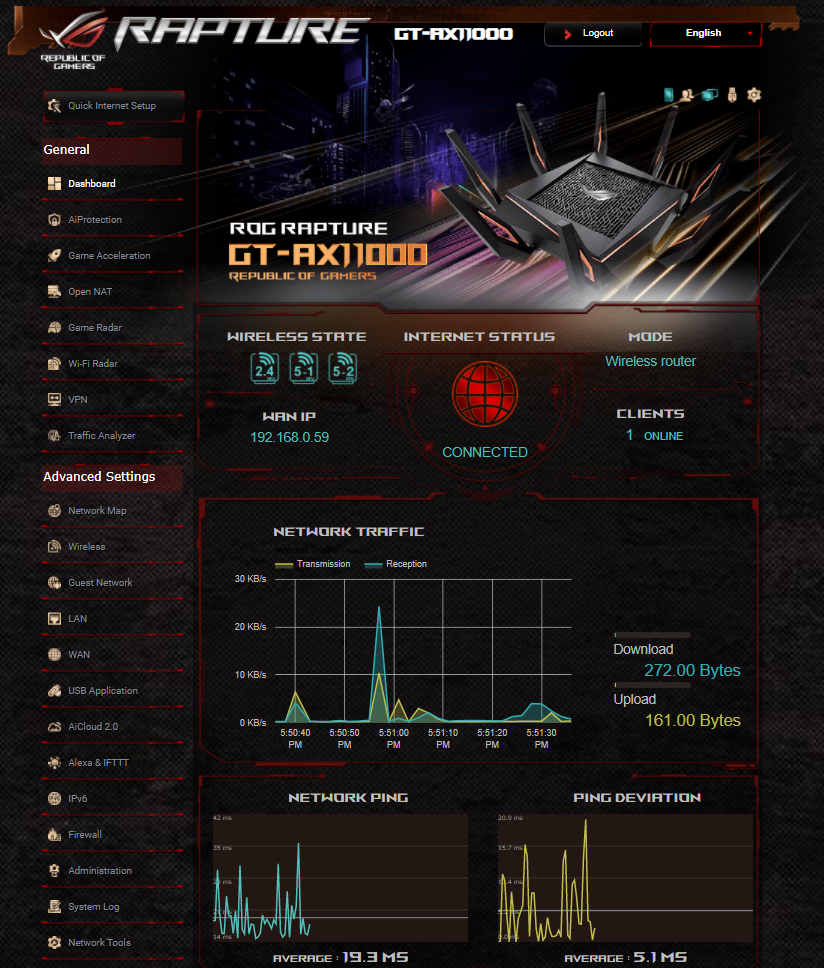
\includegraphics[width=1\linewidth]{pages/Chapter2/Chapter 2 images/ASUSwebGUI.PNG}
    \caption{ASUS ROG Gaming Centre.}
    \label{fig_ASUSwebGUI}
\end{figure}

\subsubsection{WiFi Radar}

WiFi Radar is an advanced analysis tool for the wireless network, it delves deep into the wireless channels and packet data intended for the purposes of troubleshooting. This feature permits the user to perform a Wi-Fi site survey in order to gather information on all nearby wireless access points. The site survey displays the signal strength, signal-to-noise ration (SNR), maximum physical rate, bandwidth and channel information. 




\begin{figure} [ht]
    \centering
    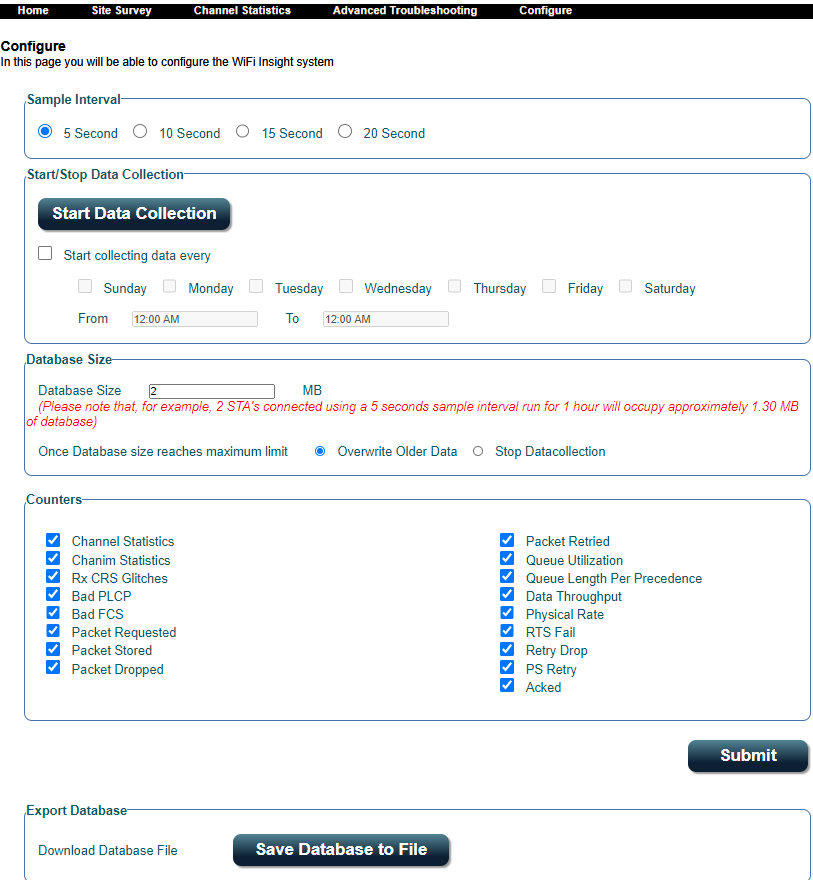
\includegraphics[width=1\linewidth]{pages/Chapter2/Chapter 2 images/WiFiRadarSetting.PNG}
    \caption{Advanced Troubleshooting Page on ASUS Web GUI.}
    \label{fig_WiFiRadar}
\end{figure}

Additionally, the Advanced Troubleshooting feature provides a telemetry data collection option, as shown in figure \ref{fig_WiFiRadar}, which produces a database with all technical data about the various advanced Wi-Fi parameters. This WiFi Radar component records data and generates a .DB file which is size configurable. This means that the user can define a maximum size that the database can reach after which it will either overwrite the older data or just stop data collection altogether. Also, the sample interval is configurable with settings to have data recorded every 5, 10, 15 or 20 seconds. Moreover, ASUS state that collecting data using a 5 second sample interval and with 2 STA’s (Stations) for 1 hour will approximately occupy 1.3MB of database, with new datasets being appended to the existing file. 

Appendix B Section \ref{ASUSEmail} shows an email correspondence with the ASUS customer service team asking to provide additional documentation for purposes of research and project work. Since ASUS could not provide additional information on what each parameter specifically measures and what the definition is for each one, research had to be conducted to fully understand what data could be extracted from the router.

Defined below are the wireless network parameters that can be recorded using the ASUS GT-AX11000 Wi-Fi router. 

\textbf{Channel Statistics}: Measures specific congestion metrics for each channel. A channel is a smaller subdivision of the WiFi frequency band through which wireless networks can send and receive data.

\textbf{Chanim Statistics}: Measure of channel interference.

\textbf{Rx CRS Glitches}: CRS (Certificate Signing Request) is a block of encoded text sent from an applicant to a Certificate Authority when applying for an SSL Certificate. It typically contains the public key for which the certificate should be issued, identifying information (such as a legal organisation name, domain name, locality and email address used to contact organisation) and integrity protection. A private key is also created at the same time as the CRS making a key pair \cite{CRS}. 

\textbf{Bad PLCP}: The PLCP (Physical Layer Convergence Protocol) maps the MAC protocol data units into a suitable frame format so they are ready for transmission by the Physical Medium Dependent. One of the other main operations of the PLCP is to route the incoming frames from the client to the MAC layer \cite{PLCP}. Bad PLCP is a receiver error metric \cite{PLCPPaper}. 

\textbf{Bad FCS}: FCS (Frame Check Sequence) is an error-detecting code added to a frame (frames are used to send payload data) \cite{FCS}. Bad FCS is the number of incoming packets where a Frame Error is detected. 

\textbf{Packet Requested/Stored/Dropped/Retired}: Count of number of packets requested, stored, dropped and retired per timestamp. 

\textbf{Queue Utilization}: A queue in networking is where packets of data ready to be forwarded are buffered before scheduling. The packets of data once in the queue are forwarded directly to the ingress (in) or egress (out) interfaces \cite{QOSPolicies}. In Queueing Theory, the Utilization factor is the amount of time that the system is busy. 

\textbf{Queue Length Per Precedence}: How many packets are transmitted between the AP and each connection, with certain packets given a priority. This is determined by the network scheduler (or packet scheduler) which manages the sequence of packets in the receive and transmit queues \cite{varghese_2005}. 

\textbf{Data Throughput}: How much data was transferred from a source at any given time (how many packets arrive at their destinations successfully). 

\textbf{Physical Rate}: The data rate obtained when data is actively transmitted. 

\textbf{RTS Fail}: When one node wants to transmit data to another node, it sends out a RTS (Request to Send) packet. The receiver node replies with a packet called CTS (Cleared to Send). After the transmitter node receives the CTS packet, it transmits the data packets. RTS Fail is the number of RTS packets sent without receiving a CTS packet response \cite{Karn1990MACAaNC}. 

\textbf{Retry Drop}: The number of attempts the wireless system makes to send a packet again before dropping the packet \cite{RetryDrop}. 

\textbf{PS  Retry}: The number of times packets are re-sent due to packet loss.  

\textbf{Acked}: Acknowledgement (ACK) is a signal that is sent by a device to show that data has been successfully transmitted, it is part of the communications protocol \cite{ackSignal}.



\section{Amazon Web Services}
\subsection{What is AWS?}
Amazon Web Services (AWS) is the one of the largest cloud-computing resources in the modern day. With many large companies using AWS as a way of bringing data and content to end-users from a server back-end on as grand a scale as necessary. On the main AWS website the following quote is shown.
\begin{quote}
\textit{Amazon Web Services (AWS) is the world’s most comprehensive and broadly adopted cloud platform, offering over 175 fully featured services from data centers globally. Millions of customers—including the fastest-growing startups, largest enterprises, and leading government agencies—are using AWS to lower costs, become more agile, and innovate faster.}  \cite{ch1_2_what_is_aws} 
\end{quote}

The above text gives an idea of the grand-scale that their services cater for with many millions being provided for. With data centres located in many regions across the globe with their own sub-regions or Availability Zones as will be discussed later. Some major companies that use AWS include \textit{Netflix}, \textit{Facebook}, \textit{LinkedIn}, and \textit{F1 Insights} to name a few. They all use AWS for content-delivery, data storage of users and website files, security and authentication and to generally manage routing of users to reduce server loads within and across regions. There also exists many abilities within AWS for disaster management (either physical or virtual) and it provides recovery tools them to ensure the end-user does not go without their service. This proof is discussed in the \textit{Gartner Report} \cite{ch1_2_amazon_is_best} that shows AWS as the best Cloud-based service for ability to deliver and completeness of services provided and gained for.

As a result of the accessibility to learn and setup the various services provided by AWS, large companies, start-ups, and research projects are able to flourish. Some of the most common services are \textit{EC2}, \textit{Lambda}, \textit{Simple Storage Services} (referred to as \textbf{S3} for the rest of the report), API Gateway, and Sagemaker to name a few of the many services. The services named here will be used within the GDP and discussed in the later sections. 

To access these AWS services, Identity and Access Management (IAM) roles are usually created first. This step can be done by accessing the IAM dashboard, which is also an AWS service itself. Each IAM role created is attached with an editable permission policy which allows users to define permissions to make AWS service requests. 

Research into other possible services and architectures were also conducted to handle the project. In the following few sections, the report will discuss case studies for how AWS has been used for IoT data collection, processing and Machine-learning environments as well as Edge-Capabilities within the industry. After this, research into the specific services and how they can be used will be discussed.

\subsection{AWS Case Studies}

The following case study takes a look at using IoT Core, which will later be used for deploying data extraction, transformation and loading functions as well for taking advantage of localised ML Models. IoT Core and all of its services can be deployed using the IoT Greengrass services, which is discussed later.

\subsubsection{Bayer Crop Science - Using IoT Core}
Bayer Crop Science used AWS to help gather real-time agriculture data from farms and to provide real-time analysis for usage by analysts, and for farmers to be able to react to changes within the environments \cite{ch1_2_case_study_1}. Initially data was collected manually from various sensors across the farm, but collating this data and analysis would take time and would eventually lead to issues not being resolved or being resolved too slowly. These issues could arise if seed deposition seized, water and feed to the crops was not being delivered correctly, harvested sections were not being correctly collected etc... With a whole host of consecutive problems that could come up if not dealt with immediately, mainly leading to reduction in harvest quantity, quality of produce and profit for the farms.

Bayer Crop Science were able to leverage AWS IoT Core, AWS Greengrass and AWS IoT Analytics to get seed data during planting and harvesting to analysts within minutes rather than days and give the farmers ample time to respond to the data and to take the actions needed. This is a case where AWS can speed up data ingestion and analysis to minutes and seconds rather than days and hours. The analysts have easy access to the data anywhere from the globe and can provide feedback to the farmers immediately. However, this solution does not fit into the category of Industry 4.0 where Machine Learning (ML) is able to assist in making decisions. In this case study AWS is only leveraged for data collection and display for an analyst to make decisions. Our project aims to further the work done by Bayer Crop Science by involving ML technologies into the system, but also to localise the ML Model. In this case, the ML Model local to the farms would be able to provide feedback in seconds rather waiting than for an analyst to analyse the hundreds if not thousands of sensor data collected depending on the scale of the farms.

\subsubsection{Sensor Networks - Predictive Analysis}
Sensor networks is an IoT Tech startup that focuses on building a platform to monitor and help home insurance companies. The company places hardware sensors onto home appliances and are able to monitor performance and to detect and minimise risk to possible breakdowns within the household \cite{ch1_2_case_study_2}. With each monitoring device connected using IoT cloud, Sensor Networks are able to collate the data into the cloud and use predictive analytics to inform home owners of any issues and possible risks and also to provide evidence for insurance claims. 

The usage of machine learning in this case study is for predictive analysis and requires large collation of data, but the processing still happens on the cloud-side. They use AWS Sagemaker, which is discussed in the later ML Technologies section to produce new models and deploy them quickly to the production stage. However, the company did not deploy the models locally for the lowest-latency response. For this company there was no need to provide analysis of the system immediately, hence it was avoided. The case study instead looks at the integration of IoT core to be able to pull data from many sensors around the household. Collate them into storage and then use the data for training and verification of models. AWS IoT core allows for all of this to happen, as well as for IoT analytics to analyse and display the data in real-time, all while supporting model deployment.

\subsection{AWS Services}
The following sections give a brief intro to the AWS Services that we plan to use throughout the project.

\subsubsection{Simple Storage Services - S3}
In order to first fully understand the benefits of S3, the types of storage must be understood. This will allow the reader to know why S3 was chosen as the primary storage utility.
\paragraph{Block Storage}
The data is separable into small blocks. (i.e. A database), in this case there might be 200 entries within this database file. Block storage allows for users to change only 1 entry and keeps the read/write requests very small for each access periods.
\paragraph{Object Storage}
Object storage allows for entire file(s) to be added, removed and read from and any small modification to a single file would result in a complete re-upload of that file. 

S3 is used for WORM operations (Write Once, Read Many) - which is very useful for website resources that do not change often. It is also good for storage of unpredictable sizes due to its vertical scalability. Since the project does not require us to send SQL data or db files around, using S3 is a clear choice, where each object to be stored is a data file optimised for transport in the telemetry pipeline. 

S3 allows for storage of objects in \textit{buckets} where each bucket \textbf{must} have a unique name in the entire region. There are several naming rules that must also be followed:
\begin{itemize}
    \item No uppercase
    \item No underscores
    \item 3-63 characters long
    \item Must start with lowercase letter or number
\end{itemize}
Once the bucket has been created, objects can be stored into it. Each object has a path associated with it known as its \textit{key}.

\begin{itemize}
    \item S3 Bucket Name: s3://my-bucket/
    \item With key: s3://my-bucket/\textbf{my\_file.txt}
    \item Object in sub-directory: s3://my-bucket/\textbf{my-folder1}/\textit{my\_file.txt}
\end{itemize}

This is the basics of setting up an S3 Bucket. The user-interface allows for easy creation and access to S3 and the setup of the buckets used is discussed further during the Implementation Section (\ref{Chapter:Implementation}). S3 also allows for object versioning within the S3 bucket to ensure data is never lost by being overwritten. This feature is not useful to us as S3 is being used to store new data files as opposed to re-writing the same file over and over. S3 also has encryption which can be done in three different ways, from server-side (SSE), client-to-server (SSE-KMS) or completely client-side (SSE-C). More details can be found in the AWS reference documentation \cite{ch1_2_s3_encryption}. 

\subsubsection{Lambda - Serverless Functions}
AWS Lambda is one of the most powerful features of AWS. Lambda has the capability for the user to deploy code and for it to spin up as many run-time instances as necessary for the amount of requests to use that function. It is defined as \textit{Serverless Computation}. Where the \textit{Serverless} feature means that the cloud provider, or AWS, is in charge of the server back-end and does not need to be managed by the user. This means writing and deploying the code is all the user needs to worry about. 

Lambda can be setup in various ways depending on the requirements, with the main ability to be triggered on various events that occur around the AWS Cloud. For instance for every new file uploaded to S3, the Lambda trigger could be setup to handle that new data. Or Lambda could be a function that runs when called from an API Request. What exactly this entails is discussed in the later exploration of API Gateway. 

The following programming languages are supported by Lambda for deployment, along with several previous versions of these languages:
\begin{itemize}
    \item .NET Core 3.1 (C\# / Powershell)
    \item Go 1.x
    \item Java 11 (Coretto)
    \item Node.js 12.x
    \item Python 3.8
    \item Ruby 2.7
    \item Provide your own bootstrap on Custom Entity
\end{itemize}
Lambda is a great resource that lets users do ETL (Extract, Transform and Load) operations on datasets or to respond to requests, which is why it is so useful for the project (i.e. for every new dataset placed into an S3 bucket, Lambda can be triggered automatically to process the data. This is explored later in the Design and Implementation sections).

\subsubsection{EC2 - Elastic Compute Cloud}
The EC2 instance is the ability to own a computing resource where you can set how much processing power you need, the amount of RAM, the OS running on the instance, and the amount of network or local storage available to the device. Each EC2 instance can be setup to run commands on startup and instances can be configured to accommodate for more users trying to access a service via the usage of Automatic Load Balancers, and horizontal scalability within EC2. Horizontal scalability is the ability to deploy new instances with the same setup immediately (versus vertical scalability which would increase the specifications of the individual instance).

\subsubsection{API Gateway - An entry point to Cloud Features}
API Gateway allows developers to setup a RESTful framework \cite{ch1_2_api_gateway} to allow for an entry point from outside of the cloud to services or resources within the cloud securely. Authentication and authorisation can be setup in order to ensure only allowed users access the resources. API Gateway also allows users to send data to Lambda functions by packing the data into the body of the HTTP(s) request  and ensuring SSL/TLS (security) certificates are present if necessary.

\subsection{IoT Core - Deploying AWS Services}
IoT Core is a set of services that allows deployment of AWS Cloud Services to featured devices. Using IoT FreeRTOS, IoT SiteWise or IoT Greengrass allows various connections to the Cloud and localisation of services to the device. Data can then be gathered by these various features into the cloud and data analysis can be performed. It is a streamlined service making it easy for large scale operations with many IoT devices out in the field or industrial work place to collect and view data. IoT Greengrass and deployment service of various Cloud services is one of the key components for this project and is explored further in the later Edge Technologies section \ref{edge_node_technologies}.



\subsubsection{Sagemaker - All things Machine Learning} 
AWS Sagemaker is a machine learning service that provides an IDE to create  a notebook instance where one can write and execute codes in Jupyter notebooks. It allows users to build and train machine learning models. Besides this, built models can be deployed and their performance for prediction can be monitored. These processes can be carried out by using the Sagemaker Python SDK or the Sagemaker SDK for Python (Boto3).

AWS Sagemaker allows access to the AWS cloud storage services such as S3 and EC2 to import datasets to train the machine learning model. An execution role is defined in the script where it grants the user permission access to datasets in cloud storage services.

Moreover, AWS Sagemaker contains several built-in machine learning algorithms for supervised learning, unsupervised learning, computer vision and natural language processing (NLP). Examples of supervised learning algorithms include:
\begin{itemize}
    \item XGBoost
    \item k-Nearest Neighbour (kNN)
    \item Factorization Machine (FM)
\end{itemize}
Examples of unsupervised learning algorithms include:
\begin{itemize}
    \item Principle Compononent Analysis (PCA)
    \item k-Means Clustering
\end{itemize}
Examples of computer vision algorithms include:
\begin{itemize}
    \item Image classification
    \item Object detection
\end{itemize}
Examples of natural language processing (NLP) algorithms include:
\begin{itemize}
    \item Neural Topic Model
    \item Latent Dirichlet allocation (LDA)
\end{itemize}
The trained machine learning model can be deployed by creating an endpoint for it. This model endpoint can then be invoked and deployed somewhere in the cloud. For example, an AWS Sagemaker model endpoint can be invoked using Amazon API Gateway and AWS Lambda. Firstly, a Lambda function which calls the model endpoint is created. An IAM execution role that includes a policy is chosen to give permission to the Lambda function to invoke a model endpoint \cite{engdahl_2008}. API Gateway triggers an event that invokes the Lambda function where it will pass provided datasets through it. Therefore, an API gateway will be created and deployed for the specific Lambda function. The testing phase comes in by using Postman, an HTTP client for test services. An invoke URL is entered onto Postman alongside with the test data which then displays the prediction results from the machine learning model.



\section{Edge Node Technologies}
\label{edge_node_technologies}
\subsection{What is Edge Computing?}

Cloud Computing offers powerful computation capabilities to almost anywhere across the globe given a fast and reliable connection. However, in a lot of remote locations, this access is not always readily available. Sometimes, critical applications require immediate response by processing and analysis. If this local environment sends data up to the cloud and waits for real-time analysis to be performed, the remote location could struggle to get any or will receive a very delayed response. One such case could be at an oil rig in the middle of the ocean with limited connectivity to the internet. If the system is monitoring pressures within its pipes and if any excess pressure is seen, then the pipes may need to be bled out. However, to recognise this change in pressure over time previous data and all new data needs to be seen. If any immediate response is needed to change the pressure in the pipes, sending this data to the cloud would not have the required latency response as would be expected in such a crucial system to ensure system stability.

Besides, with the rapid development of Internet-of-Things (IoT), all kinds of electrical devices such as sensors and Internet-connected devices have become the data producers at the edge of network, generating more than billions of information within few years. Overwhelmed with enormous data generation simultaneously, data transportation has been a bottleneck for the traditional cloud computing, resulting not only latency due to the longer processing time but also overloading its network transmission bandwidth \cite{lei_roy_xiaoming_stefano_zbigniew_hannes_2013}. For example, an autonomous vehicle which drives itself to the predetermined destination, requires real-time processing to make correct decisions. It produces about one Gigabyte of data per second \cite{mark_2013}. If these huge data were to be sent to the cloud for processing, the response will take a longer time.

The solution to solve this problem is to have the processing and data analysis localised on the environment. However, ensuring reliability, rolled-out updates, secured data collection and from many different devices simultaneously are the main difficulties in this solution rather than having each sensor just being connected to the cloud directly and send data that way, which was just discussed could have disastrous latency-specific response issues. This solution is known as Edge Computing according to Shi et al. \cite{w_h_q_w_2017}, 

\begin{quote}
    \textit{"Edge computing is a new computing mode of network edge execution. The downlink data of edge computing represents cloud service, the uplink data represents the Internet of Everything, and the edge of edge computing refers to the arbitrary computing and network resources between the data source and the path of cloud computing center."}
\end{quote}

IoT devices that collect data (such as network or security measurements) would send their data to this local hardware running a server. This local server would contain processing, storage and networking capabilities that would allow connectivity to and within the entire remote location. One can reliably ensure that any control systems get the reliable and response they need in the correct time. 

\subsection{Edge Native Application}
Deployed to the edge of network with its extended cloud services, edge native application usually takes up one or more attributes of Edge Computing which are bandwidth scalability, low-latency offload, privacy-preserving denaturing and Wide-Area-Network (WAN) failure resiliency \cite{satyanarayanan_klas_silva_mangiante_2019}. Comparing most of the studied edge native application, there are four main categories of the application:  
\begin{itemize}
    \item \textbf{Single User Interactive}: An independent application with a single instance that execute through a user equipment (UE) in a single location. The simultaneous interaction between users over the same network/services is negligible. Our research focuses on this edge native application.
    \item \textbf{Multi-User Interactive}: The advancement of the single user interactive application with many similar features and additional characteristics where the edge application is formed by a group of edge applications. For example, multi-player video gaming. 
    \item \textbf{Edge Analytics}: Application where data collection and processing by distributed UEs were transferred to a centralized location to gain insight that drive operational action. However, it has implications of cost and latency in data transmission. Examples include intelligent processing of surveillance videos.
    \item \textbf{IoT sensors}: Application where data from the distributed sensor and UEs was collected for the analytic functions in order to provide control and assist. Examples are autonomous vehicles and distributed traffic monitoring services. 
\end{itemize}

\subsection{Instrumented Client Application}

AWS provides its own Edge Computing solution to their own Cloud services. Using IoT Greengrass, one can deploy Lambda functions, local resource access, device connectivity (e.g. to Sensors, Cameras, Network cards etc...). Greengrass allows functionality such that you can set up a group via the online dashboard. A deploy option is available in the online dashboard where  every device with the Greengrass Core installed and with access to the Greengrass group via correct certifications will update when a connection to the cloud can be established when the option is selected. Implementation of this is shown later in the implementation section.

Greengrass allows developers to use their Cloud-Based Lambda functions and deploy these of the device allowing that the runtime environment is setup on the device. E.g. In order to run NodeJS Lambda Functions, one has to install the prerequisites and ensure Node version 12.x or similar is setup on the device. While this can be seen as tedious, it is in the developers hands to be able to automate this process by using scripts to set up the Greengrass core as well as any runtime libraries required.

Specialize in monitoring, analysis and control over the networks, the AdvantEDGE edge emulation platform is able to build frameworks for modelling and measuring edge computing infrastructure as a tool for application characterization to provide strong basis of understanding and improvements on how the networks behaved in real world based on simulated environments. The modelling focuses on applying the network characteristics such as latency, jitter, packet loss and data throughput to measure the performance and quality of network system in delivering the service to the network users. The system design and implementation of the applications will be discussed further in the document.

%Research into what AdvantEdge is and how it can be used to emulate edge-nodes and network configurations to edge nodes
\section{Machine Learning}
\subsection{Introduction}
Machine learning, also known as statistical learning is the study of different types of algorithms. 
\begin{quote}
\textit{It's an integral part of many commercial applications and research projects today, in area ranging from medical diagnosis and treatment to finding your friends on social network.} \cite{muller_guido_2016}
\end{quote}
Several stages are involved in the machine learning process where it starts with identifying the problem followed by data collection, data analysis and pre-processing, feature extraction, machine learning model development and ends with performance evaluation of the model. The model would then be deployed after achieving a rather good performing benchmark.
Machine learning can be divided further into three classes which are unsupervised learning, supervised learning and reinforcement learning. In a supervised learning algorithm, each data set provided belongs to a particular class. In simple terms, an input variable, x exists along with an output variable, y where the algorithm will map the input variable to the output variable. This concept can be expressed with a simple equation in \ref{eq:1}. 
\begin{equation}
    y = f(x)  \label{eq:1}
\end{equation}
Moreover, supervised learning can be further broken down into classification and regression. Classification is used to classify or predict the class of each data while regression is used to predict a continuous output variable from a number of independent variables \cite{abrams_2007}. Examples of supervised learning algorithms are k-nearest neighbour (kNN), support vector machine (SVM) and XGBoost.  

Next, unsupervised learning algorithms are used to study pattern of datasets which do not have labels or classes. Clustering and anomaly detection are examples of unsupervised learning. “On the other hand, reinforcement learning is a process of training machine learning models giving them the ability to make decisions in a sequence” \cite{osinski_budek_2018}. 

\subsection{Processes}
\subsubsection{Data Collection, Analysis and Pre-processing}
Before training and building a machine learning model, a problem should be identified and defined. Datasets related to the problem are then collected, analysed and pre-processed. Data collected can exist in the form of categories, time-series, text and numbers. Datasets collected contain a large number of features most of the time and useful features are only required. Therefore, data analysis is carried out to search for correlation between features and the target variables or classes. Several data analysis methods can be carried out such as producing a correlation matrix, histograms, bar plots and scatter plots \cite{kashnitsky_2019}.

A correlation matrix shows the coefficient between two parameters in a N x N matrix where N represents the number of parameters. The Pearson's correlation coefficient is used and represented with the symbol \textit{r} and exist in the range of $-1\leq r \leq 1$. It measures the strength and linear relationship between two variables \cite{corr}.  The strengths of the correlation coefficients can be shown in table \ref{table:corr}. 

\begin{table}[h!]
\centering
\begin{center}
\begin{tabular}{ |c|c| } 
 \hline
 Correlation coefficient & Correlation strength\\ 
  \hline\hline
 1.0 & Very strong positive relationship\\ 
 0.8 & Fairly strong positive relationship\\ 
 0.6 & Moderate positive relationship\\ 
 0 & No relationship\\ 
 -0.6 & Moderate negative relationship\\ 
 -0.8 & Fairly strong negative relationship\\ 
 -1.0 & Very strong negative relationship \\ 
  
 \hline
\end{tabular}
\caption{Correlation coefficients strength}
\label{table:corr}
\end{center}
\end{table}
In the data pre-processing stage, anomalies would be removed. For missing data values, they are either removed or replaced with a null value. Time-series data that exists as signals will be filtered to remove unwanted noise or frequencies. The data would then be normalized or standardized to obtain data uniformity. Normalization is a process that scales values to a range between 0 and 1 while standardization scales values to be centered around the mean with a standard deviation of 1 \cite{norm_stand}. These processes are usually effective on distance-based algorithms such as k-NN. 

\subsubsection{Training, Validating and Testing phases}
The training, validation and testing phases will be performed with the preprocessed and filtered data with useful features. The dataset prepared is commonly split into ratios of 90:10 where 90\% of the data will be further split into a 80:10 ratio that will be used to train and validate the machine learning model and 10\% of the remaining data will be used to test and evaluate the built model. Other commonly used ratios used include 70:15:15 and 60:20:20. A validating set is used to evaluate the model which allows users to tune the hyperparameters to achieve a better performance. The final performance of the trained model will then be evaluated with the test data. 
\subsection{Supervised Algorithms}

\subsubsection{k-Nearest Neighbour}
K-nearest neighbour is a simple supervised learning algorithm that is frequently used for classification and regression problems. This algorithm works by simply storing the training dataset provided. It predicts or classifies a new data point by searching for the closest data points in the training data set - its ``nearest neighbors'' \cite{muller_guido_2016}.

The hyperparameters that are used for this algorithm are the distance function and number of neighbours, k. The number of neighbours is a parameter which takes the \textit{k} closest training points in the model to predict or classify a given test point. A distance function is the measure of distance to map a training point to a test point. Several examples of distance functions used are the Manhattan, Euclidean and Minkowski distance functions. The Euclidean distance function is widely used and is said to represent the shortest distance between two points in a N-dimensional space. The corresponding function can be represented by the expression in 
\ref{eq:2} where x represents the training point of the model, y represents a test point while n represents the dimension of the vector space (no. of features). 
\begin{equation}
    d(x,y) = \sqrt{(x_1^2-y_1^2)+(x_2^2-y_2^2)+....+(x_n^2-y_n^2)} \label{eq:2}
\end{equation}

An example where two classes, class A and class B exist in a trained k-NN model is shown in \ref{fig_knn}. The model with a \textit{k} value of 1 classifies a new data point by mapping the closest one training point from Class A to the test point.

\begin{figure} [ht]
    \centering
    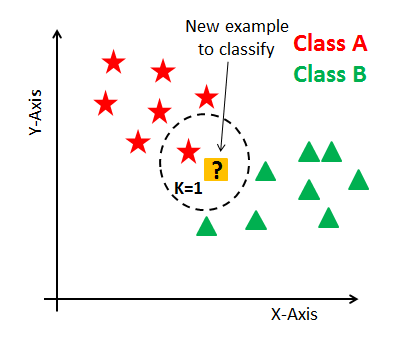
\includegraphics[scale=0.6]{pages/Chapter2/Chapter 2 images/knn.png}
    \caption{Classification of a test point with kNN. \textit{Sourced from} \cite{chauhan_2019}.}
    \label{fig_knn}
\end{figure}
 
\subsubsection{XGBoost}
XGBoost which is also known as ``\textit{e\textbf{X}treme \textbf{G}radient \textbf{B}oosting}" is a type of supervised learning algorithm used in machine learning. It is the implementation of gradient boosting machines or boosted decision trees where it heavily focuses on optimization and scalability. The XGBoost algorithm is used to solve regression and classification problems. This algorithm uses the concept of decision trees where features are split further into intervals to classify data in the form of nodes and branches.

The hyperparameters of this algorithm includes the number of classes involved, learning rate, gamma and subsamples. The number of classes represents the number of target variables available in the data provided. The learning rate prevents the overfitting of data where the trained model is only able to predict values that exist in the the training set.
Overfitting implies that the model trains by including noise or existing anomalies in the provided dataset. The subsample and gamma hyperparameter shares the similar concept as well to prevent overfitting of the machine learning model. 

\subsection{Machine Learning Model Performance Evaluation}
The final performance of the machine learning model will be evaluated using the split test data. Metrics such as the confusion matrix can be used to measure the performance of the trained model. Several parameters can be obtained from the confusion matrix such as accuracy, sensitivity, precision and specificity. The confusion matrix is a N x N matrix which shows the number of classified and misclassified data for N classes of data. An example of a confusion matrix can be shown in \ref{fig_cf}.

\begin{figure} [ht]
    \centering
    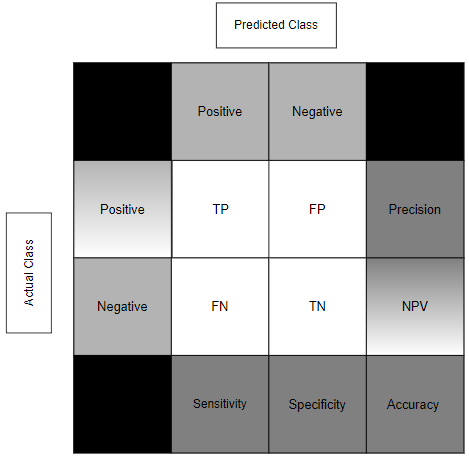
\includegraphics[scale=1.0]{pages/Chapter2/Chapter 2 images/Confusion matrix.PNG}
    \caption{Confusion matrix.}
    \label{fig_cf}
\end{figure}

From fig. \ref{fig_cf}, TP, FP, FN and TN represents true positive, false positve, false negative and true negative respectively. True positive and true negative represent data predicted correctly with the actual class while false positive and false negative are misclassified data predicted under the in incorrect class.
The accuracy of the model which represents the data are classified under the correct class can be evaluated with \ref{eq:3}.
\begin{equation}
    Accuracy(\%) = \frac{TP + TN}{TP+TN+FN+FP} X100\% 
    \label{eq:3}
\end{equation}

Specificity measures the frequency of data predicted correctly under the negative actual class as shown in \ref{eq:4}. 
\begin{equation}
    Specificity(\%) = \frac{TN}{FP+TN} X100\% 
    \label{eq:4}
\end{equation}

Sensitivity shows the data correctly under the positive class and can be computed  with \ref{eq:5}.
\begin{equation}
    Sensitivity(\%) = \frac{TP}{TP+FN} X100\% 
    \label{eq:5}
\end{equation}

Thus, the confusion matrix is one of the several useful metrics to determine the performance of a machine learning model before getting it ready for deployment.





%     1. Introduction including the following points: (i) what is the required product and how it will be applied. The name of the organisation of the external partner and names of the contact(s) (ii) why the product should be created (Societal, environmental, economic (competing technologies and advantages over these?) (iii) the main field, technology area of your external partner and the rational as to why the external partner wishes for the product to be created and who will exploit it (non-expert/expert, other engineer/research area) (iv) Clearly identify whether the output required by the external partner is a 'proof of concept', demonstrator or application of an existing technology (for a trade show for instance), a prototype or an elaboration or add-on of/intergration with/ superseeds an existing system.






%% ----------------------------------------------------------------
%% Introduction.tex
%% ---------------------------------------------------------------- 
\chapter{System Design} \label{Chapter:System Design}
% Need an introduction to the system design - referencing to system diagrams generated
Following the brief outlined in \ref{0_2_project_brief}, the system diagram shown in Figure \ref{fig_system_diagram_full} allows the system to be split into three different stages, with a fourth stage for any application derived from the data and from any classifications made by the ML Model developed. 
\begin{enumerate}
    \item Data Collection and Transformation
    \item Localised Processing, Storage and Classification
    \item Cloud Based Processing, Storage and Inference
    \item Over-the-top Application using ML Model Outputs and Input Data
\end{enumerate}



\begin{figure}[ht]
    \label{fig_system_diagram_full}
    \centering
    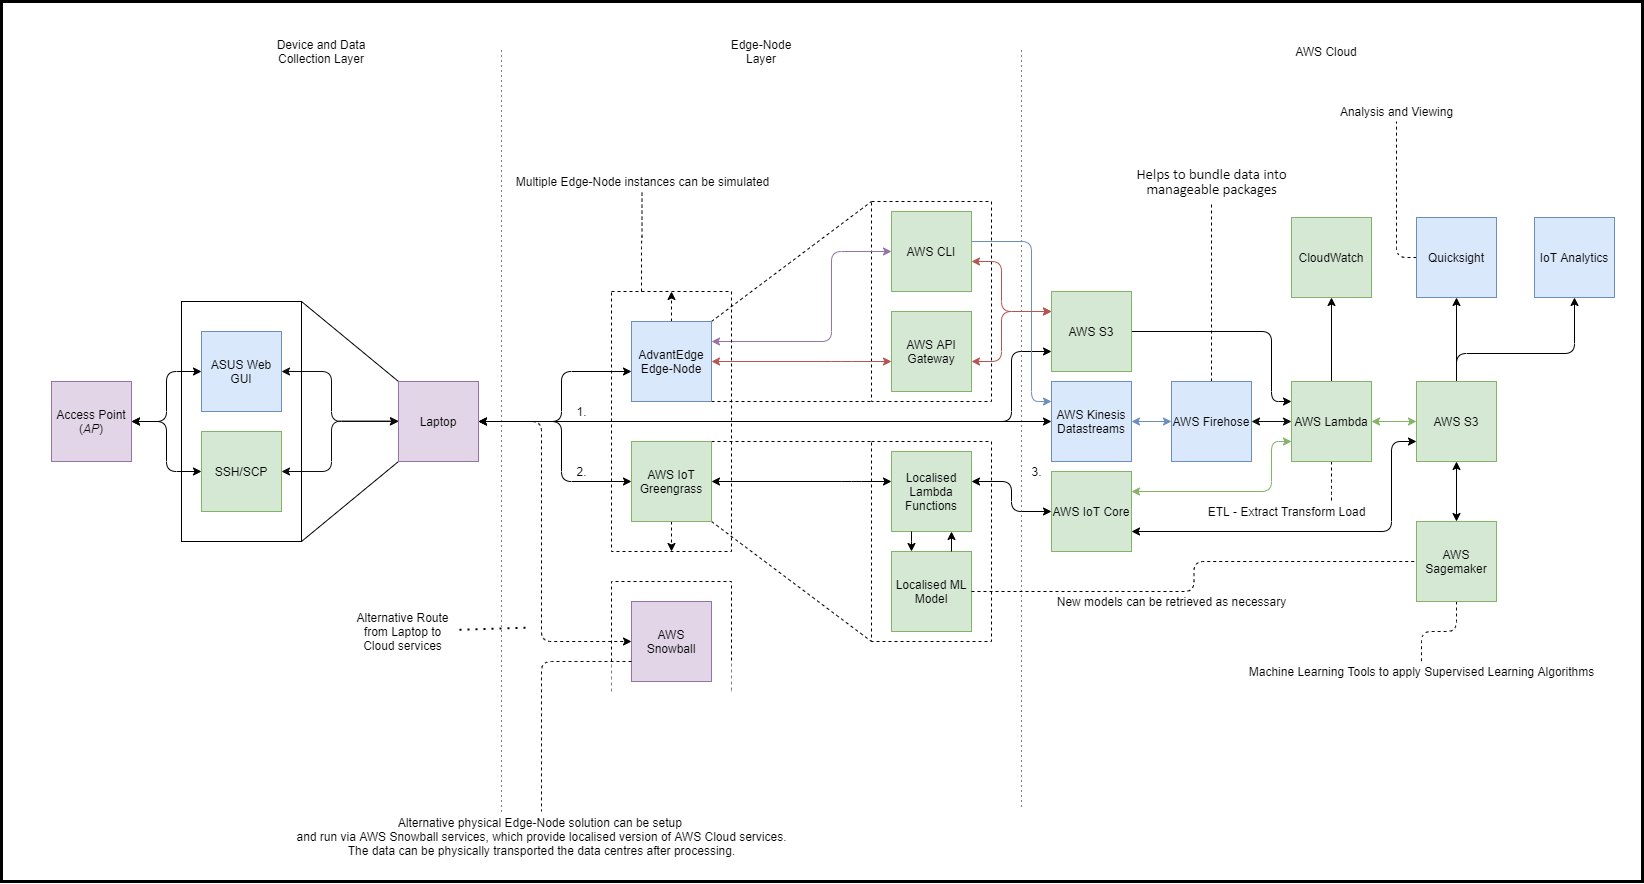
\includegraphics[width=1\linewidth]{pages/Chapter3/Chapter 3 images/block_system_diagram_v2.png}
    \caption{Full System Diagram - The full scale diagram is in Appendix A [\ref{appendix:full_scale_system_diagram}]}
\end{figure}

From these 4 stages, the system design can be understood. All data is collected from the access point, which for this project is ASUS Rog AX11000 Router, which is connected to a laptop and is responsible for data retrieval. The laptop in this wireless pipeline is an end-user connected to some access-point. The project then explores data transportation through several data pipe-lining methods..
\begin{itemize}
    \item Data is sent directly to the cloud from the Laptop after data is compressed into a smaller and better format for transport.
    \item Data is sent to a local Edge Node containing processing and ML models to process data and all analytics and results are computed direclty on the Edge Node.
    \item Data is sent to the cloud from the laptop via the Edge Node. Comparisons in latency of response can easily be drawn from this.
\end{itemize}

In the following few sections, the report will explore each of these stages metnionted above as well as how data will be processed in each pipeline path.

\section{Data Collection and Transformation}
\label{data_collection_design}
% Need to discuss db -> json files
% Compression of json files into 1 json file
% Conversion into format for ML format
% \usepackage{arydshln}

Following on from the research conducted into the wireless network parameters that can be recorded using the ASUS ROG router (Section \ref{section:WirelessTelemetryResearch}), the next step is to design the system to utilise all relevant data. 

\subsection{Data Categorisation}
\label{Section: Data Categorisation}

\begin{figure} [ht]
    \centering
    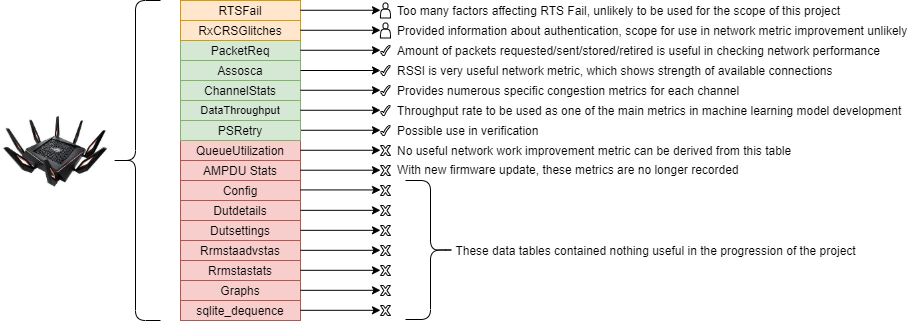
\includegraphics[width=1\linewidth]{pages/Chapter3/Chapter 3 images/router_data-Datasets-Usefulness.png}
    \caption{Database file table categorisation. Full  scale  diagram  can be seen in Appendix A Section \ref{appendix:ASUS router datatable}.}
    \label{fig_ASUSDatatables}
\end{figure}

The first stage of this process is to categorise the data into three sections; relevant data to be used in machine learning development \& deployment, data with potential but specific use cases and redundant data. The database (.db) file generated by the ASUS router, catalogs the data parameters into separate data tables as shown on the left hand side of Figure \ref{fig_ASUSDatatables}. The tables marked in red are either redundant data providing no useful insights into network performance or data through  which no meaningful information can be derived. Tables marked orange present beneficial information with potential for use but are not within the scope of this project. hence will not be further considered. Tables marked green all provide useful information through which network characteristics can be analysed and will be further studied for the purposes of Machine Learning model and OTT application development.  


The next step in this system design process was to understand how each table in the .db database file was organised. Each table starts with a column titled "rowID" labeled 1 - 3, which correspond to the current operational frequency band (5GHz-1, 2.4GHz and 5GHz-2 respectively). Then the individual data parameters are classified under a column titled "GraphrowID" labeled 1 - 17 which define what each dataset in the table represents. Table \ref{table:GUIData} shows the GraphrowID values and their corresponding parameter, unit and table name. 


\begin{table}[h]
\centering

\begin{tabular}{:l:l:l:l:} 
\hline
\multicolumn{1}{|l|}{\textbf{GraphrowID}} & \multicolumn{1}{l|}{\textbf{Parameters}} & \multicolumn{1}{l|}{\textbf{Units}} & \multicolumn{1}{l|}{\textbf{Table Name}}  \\ 
\hline
1                                         & Congestion                               & Percentage                          & ChannelStats                              \\
2                                         & Chanim Statistics                        & Count                               & ChannelStats                              \\
3                                         & Rx CRS Glitches                          & Count                               & RxCRSGlitches                             \\
4                                         & Bad PLCP~                                & Count                               & RxCRSGlitches                             \\
5                                         & Bad FCS                                  & Count                               & RxCRSGlitches                             \\
6                                         & Packet Requested                         & Count                               & PacketRequested                           \\
7                                         & Packet Stored~                           & Count                               & PacketRequested                           \\
8                                         & Packet Dropped                           & Count                               & PacketRequested                           \\
9                                         & Packet Retired                           & Count                               & PacketRequested                           \\
10                                        & Queue Utilisation~                       & Count                               & QueueUtilisation                          \\
11                                        & Queue Length Per Precedence              & Count                               & QueueUtilisation                          \\
12                                        & Data Throughput~                         & Mbits/s                             & DataThroughput                            \\
13                                        & Physical Rate~                           & Mbits/s                             & DataThroughput                            \\
14                                        & RTS Fail~                                & Count                               & RTSFail                                   \\
15                                        & Retry Drop~                              & Count                               & RTSFail                                   \\
16                                        & PS Retry                                 & Count                               & PSRetry                                   \\
17                                        & Acked                                    & Count                               & PSRetry                                   \\
%\hdashline
\end{tabular}
\caption{ASUS ROG Router Data Table\\}
\label{table:GUIData}
\end{table}

\subsection{Database File Conversion}
\label{Section: Database File Conversion}

Now with a better understanding of all the parameters that can be recorded through the ASUS router and having established which parameters will be further considered, the next step is to convert the database file into a more appropriate format. A .db file is typically used on mobile devices and is not intended to be opened or edited manually \cite{dbFiles}, because of this the .db file format is not suitable in the development of the telemetry pipeline plus it is not compatible with AWS. For this three other file formats were considered CSV, XML and JSON. The CSV (Comma Separated Value) format is a delimited text file which uses commas to separate out values. Each line of the file is a record and each record is compromised of one or more fields separated by commas. CSV files are best used to represent data in which each record has an identical list of fields with a single relation, and databases which have multiple relations cannot be exported to a single file. Hence the best use case is when the data has a strict tabular structure and when very large databases are required to be transferred between programs. XML (Extensible Markup Language) is a self-defining file format, meaning the structure of the data is embedded within the data itself, therefore when the data arrives at the destination there is no need to pre-build the structure. Due to its platform independent nature XML simplifies the data transfer process as there is no further conversion necessary when transferring between different systems. However, the syntax for XML is verbose and the redundancy in the syntax results in higher storage and transportation costs. JSON (JavaScript Object Notation) is a lightweight text based file and data interchange format which uses human-readable text to store data objects. It is primarily used to transmit data between a server and web application due to the fact that JSON provides easy parsing and faster execution of the data. 

With the three file formats researched and better understood, the decision was made to convert the .db file into the JSON format for further use in the development of the telemetry pipeline. CSV was not chosen as it does not provide the ability to have relational databases. Also XML was not chosen as it added redundancy to the data with its verbose syntax, hence it would not be appropriate in a system where efficiency and low latency was critical to its operation. Furthermore, with the ability of JSON to use less data resulting in increased parsing and execution speeds it was chosen as the main file format in this project. 


\subsection{JSON File Compression}
\label{Section: JSON File Compression}


With the way in which the .db file generated by the ASUS router is organised, each relevant data table needs to be read into separately. This means that in the conversion stage, every data table that is converted will produce its own JSON file. These individual JSON files are to be used in the direct upload to the S3 data storage, where it will be further processed on the cloud. However, on the edge node side of the system these distinct JSON files must be combined and compressed into a single file for further use. As well as this further compression and removal of unnecessary data is required for use in Machine Learning model. 

\subsubsection{JSON Conversion Keys for Each Table}

\textbf{\underline{ChannelStats}}

[rowID, TimeStamp, Channel, tx, inbss, obss, nocat, nopkt, doze, txop, goodtx, badtx, glitch, plcp, noise, idle]

\textbf{\underline{Assocsta}}

[rowID, TimeStamp, "MAC", RSSI, PhyRate]

\textbf{\underline{DataThroughput}}

[rowID, GraphrowID, "MAC", TimeStamp, "XAxis", " Data Throughput/Physical Rate"]

\textbf{\underline{PacketRequested}}

[rowID, GraphrowID, "MAC", TimeStamp, "XAxis", " Packet Requested/Stored/Dropped/Retired"]

\textbf{\underline{PSRetry}}

[rowID, GraphrowID, "MAC", TimeStamp, "XAxis", " PS Retry/Acked"]

\subsubsection{JSON Key for Compressed File}
 
\{\\
"DeviceID - GraphrowID": "value",\\
...\\
...\\
...\\
"Channel Number - Channel Stats": "value",\\
...\\
...\\
...\\
"TimeStamp": "value"\\
\}

\subsubsection{JSON File Key for ML Model Compatibility}

['Packet Requested', 'Packet Stored ', 'Packet Retired', 'BADTX', 'GOODTX', 'TX', 'TXOP']



\section{Localised Processing, Storage and Classification}
% Discuss Lambda functions deployed to the Edge and how they interact
% Discuss how web server can see data throughout the greengrass
% Discuss how AdvantEdge can help validate results within the model
% 

\subsection{Edge Node Design}
For the Edge Node design, following the research into Edge Computing in Section \ref{edge_node_technologies} and seeing that AWS IoT Greengrass is a great solution to bringing Cloud Features to the edge, it was understood that we needed processing, network capabilities, and ability to work while not interrupting the user experience. 

IoT Greengrass lets us do exactly that, IoT Greengrass is meant to be run on devices that support embedded Linux Systems, such as a Rasperry Pi, NVIDIA's Nano Jetson or Intels Atom Board to name a few. To show that our system works for any embedded system, the project places Greengrass onto a virtualised linux system running on x86\_64 architecture. However, support exists for many  other hardware architectures and OS's.
\begin{figure}[ht]
    \centering
    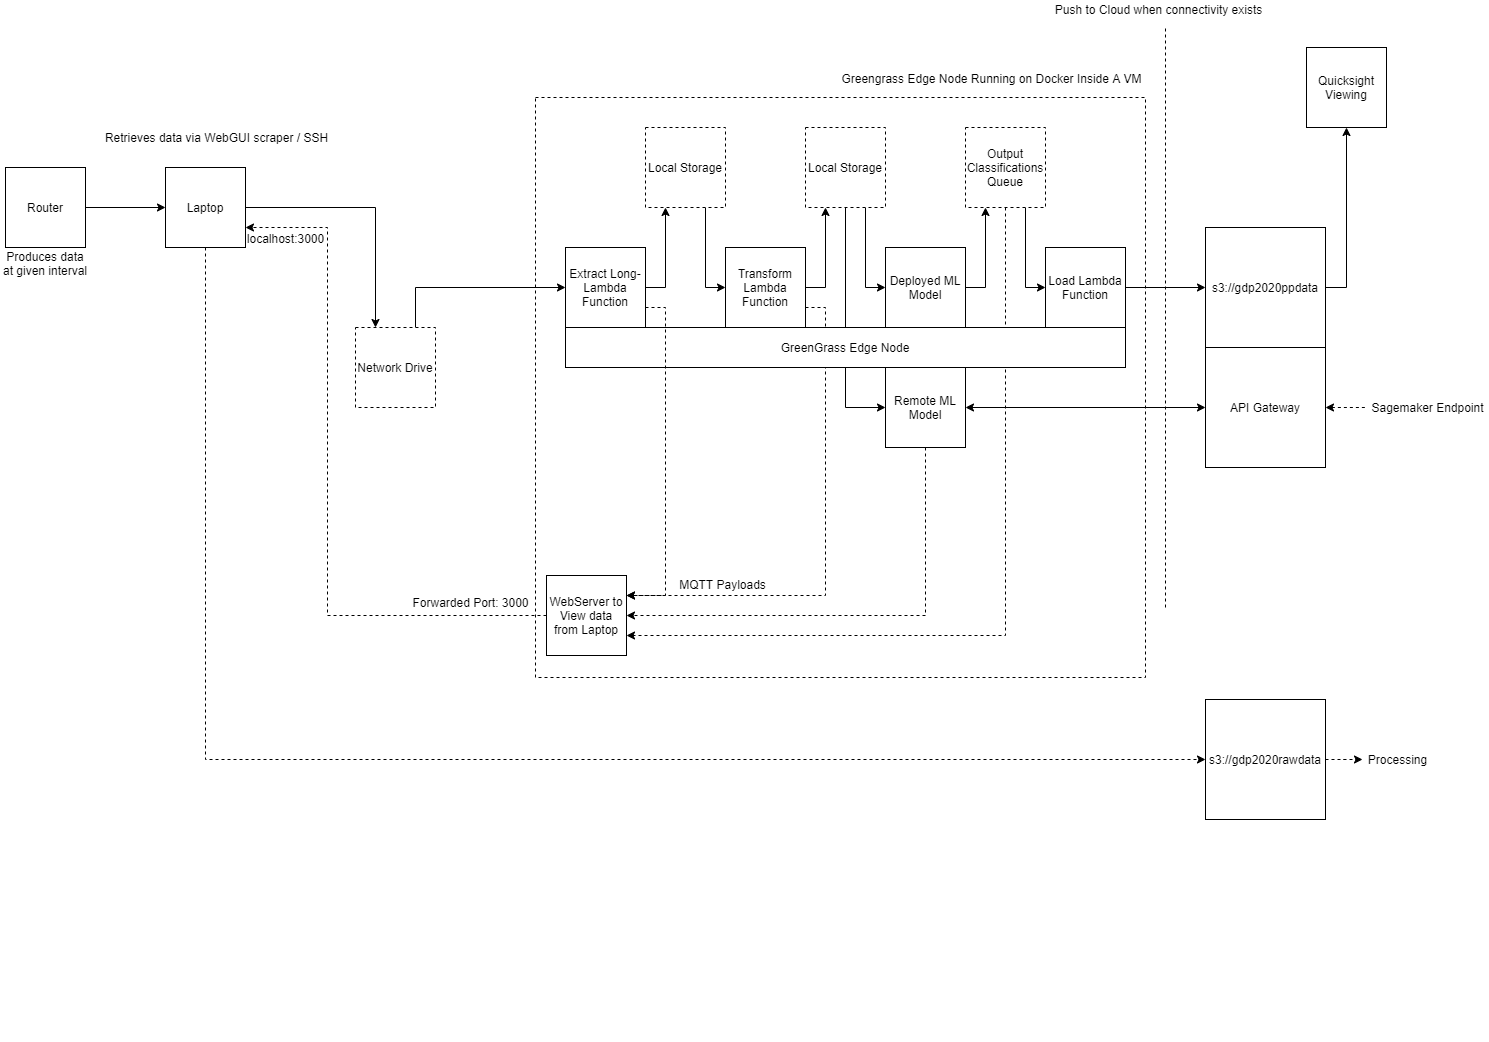
\includegraphics[width=1\linewidth]{pages/Chapter3/Chapter 3 images/greengrass_data_flow.png}
    \caption{The data flow within the Local Environment for Edge Computing -\textit{ The full scale diagram can be seen in Appendix C} [\ref{appendix:greengrass_design}]}
    \label{fig:greengrass_edge_design}
\end{figure}

From the design in Figure \ref{fig:greengrass_edge_design}, we can see how the system will function for 2 out of the 3 pipelines discussed earlier.
\begin{enumerate}
    \item Data is collected from the Router and stored in some (local) network data storage facility.
    \item This data is then retrieved by the Extract Lambda function running at the Edge and is stored locally.
    \item The Transform Lambda function will then begin the pre-processing of the data for usage and analysis.
    \item The Load Lambda function takes the pre-processed data and transfers it to the S3 Pre-Processed-Data bucket on the cloud.
    \item Pre-processed data is also taken to the ML-Inference Lambda function which uses an obtained ML Model from the Cloud for local classification of the data.
    \item Pre-processed data is used and a request is sent to the cloud for classification. Timings between Local ML-Classification and Remote ML-Classification can be compared
    \item All data is sent to a local web-server showing all timings and classifications being made by the functions described
\end{enumerate}

The first point is discussed earlier in Section \ref{data_collection_design} and how data can be collected. Point two discusses the extract function. The laptop and the edge node share a network folder within the the local environment. Data to be sent to the Edge Node will be placed into the shared folder by the laptop. In this case it is the raw data in the (.db) file format obtained from the router that is placed in the shared folder. The extract function will then take the database file and convert each data table within the database into its own JSON file.

The third item discusses the transform function. This function \textit{compresses} all the JSON files that were extracted from the database file into a single array of all data elements corresponding to a single timestamp value as described in Section \ref{data_collection_design}. 

The fourth item describes the load function. Since Edge nodes are often resource constrained in terms of hardware, either in processing power, memory available or data storage. It is often required to upload the data to the cloud upon good connectivity to ensure data is not lost and can be used for long-term analytics. The load function will then use API Gateway to securely send data to an S3 bucket to store the pre-processed data for any cloud-based processing and training of ML models. The load function allows for one of the two pipelines to be completed where data is transferred to the cloud via the Edge node rather than directly from the laptop. The sixth item is also a part of this pipeline where data can be sent to a cloud endpoint where Sagemaker has deployed a ML model to classify data. 

The fifth item discusses using a deployed ML Model that runs on the local edge node. This model is developed on the cloud using data that has been collected previously for training and verification of the model. This model can then be deployed using Greengrass where the model can be taken from any S3 bucket and then transported to the edge node. More about the model development is discussed in Section \ref{cloud_services}.

The final item in the list discusses the front-end of the Greengrass Edge node. This is a custom solution to being able to view all the data in real-time for analysis or for any OTT application to be built on top of. The data is passed around from each Lambda function using MQQT packets. Each Lambda function can subscribe to a topic. E.g. 'server/extract/data'. And on this topic, another Lambda function can publish a message for it to be read by the subscribers. These data packets can all be seen by viewers on the cloud and so other services via AWS SNS are able to subscribe to these topics and then react accordingly especially for data viewing or analytics. For this project however, a custom GUI has been designed therefore a custom OTT Application could be implemented a top of it.

\subsection{AdvantEDGE}
AdvantEDGE is a mobile edge emulation platform (MEEP) that runs on Docker and Kubernetes where all the micro-services interacted together were packaged in Docker containers before deploying in the Kubernetes pods to the AdvantEDGE for the edge scenarios testing. AdvantEDGE provides an emulation environment that enables experimentation on the edge computing technologies, applications and services. The platform facilitates exploring edge deployment models and their impact on applications and services in short and agile iterations. The user enables to define a scenario that includes:
\begin{itemize}
    \item A network topology of cloudlets, operators, wireless points of access (PoA), zones and UEs.
    \item Network characteristics for each of the elements set up including latency, jitter, packet loss and data throughput.
    \item Network and mobility events to change network characteristics and the location of UE and cloudlets during simulation run time. 
\end{itemize}

It allows the connection of real physical cloudlets and edge/fog/UE applications so that the simulation can capture the impact of the network design on its application performance. It also supports event scripting, collection of measurements in third parties such as an offline InfluxDB time series database and real time Grafana dashboards. AdvantEDGE platform and instrumented client load data into InfluxDB time series database where AdvantEDGE stores network and event measurements from deployed scenarios. Grafana dashboards were primarily used to monitor scenario execution and demonstration purposes. This combination makes it powerful platform for the edge network simulation.

\begin{figure}[ht]
    \centering
    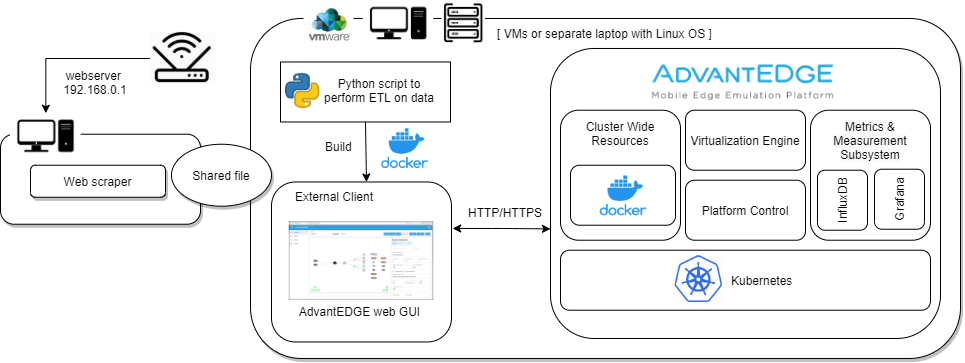
\includegraphics[width=1\linewidth]{pages/Chapter3/Chapter 3 images/System Diagram.png}
    \caption{The system diagram of edge application deployment to the AdvantEDGE}
    \label{fig:AdvantEDGE_edge_design}
\end{figure}

Figure \ref{fig:AdvantEDGE_edge_design} shows the proposed system diagram of edge application deployment on the AdvantEDGE. The data collected from the router will be accessed to the VM through shared file, where python scripts will extract these data to convert from .dB into json files, then perform transform function to compress these json files into one before loading json file into ML model for evaluation. To be able to use the functionality of the mobile edge emulation platform, these python applications will need to be built as Docker images before deploying them as a native edge application.


\section{Cloud Based Processing, Storage and Inference}
\label{cloud_services}
%Need to discuss Lambda which takes raw data to pp data bucket here
\subsection{Laptop to Cloud Pipeline}
\subsubsection{API Gateway}
In this section we discuss the entry way into the AWS Cloud. The API Gateway allows us to take any data produced the Edge location either from the end-user or the Edge nodes deployed and securely redirect them to storage and analysis endpoints. Figure \ref{fig:api_gateway_methods} shows how various URLs an be used to upload and send data to different buckets or endpoints. Usage of Sagemaker's endpoints are discussed later, but to get data from the edge to the cloud, the S3 endpoints are used by API Gateway. For example, doing a \textit{PUT} request to the provided URL from API Gateway, with the body of the request filled with the JSON object to be uploaded, would store the data file with the new Key value into the requested S3 bucket.

\begin{figure}[ht]
    \centering
    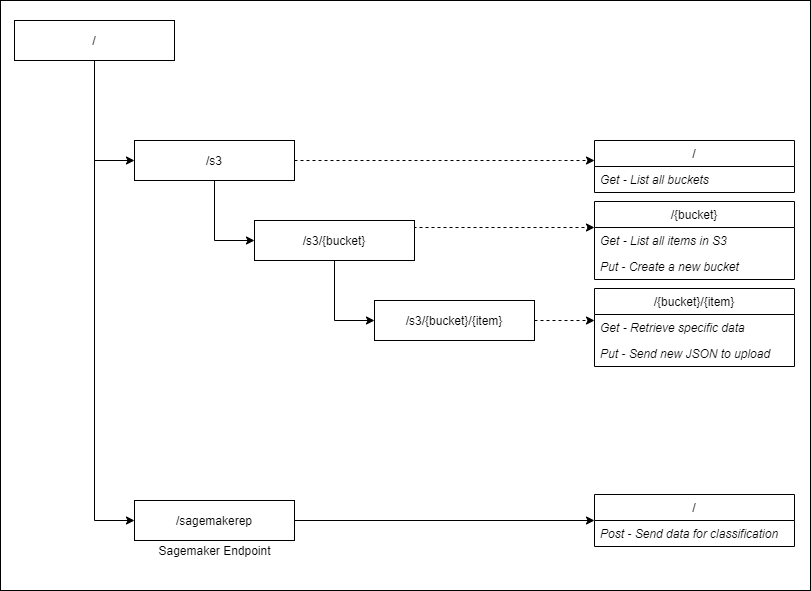
\includegraphics[width=1\linewidth]{pages/Chapter4/Chapter 4 Images/api_gateway_1.png}
    \caption{API Gateway Resources and Attached Methods}
    \label{fig:api_gateway_methods}
\end{figure}


\subsubsection{Lambda - Data Pre-processing on the Cloud}
\label{cloud_lambda}
Once the data has been prepared and the API Gateway setup, then Lambda services can be triggered to react to New Object events on S3. It can be setup such that every new object will trigger the Lambda function, however it may be the case that not all the 5 JSON files will have been uploaded as part of the Laptop to Cloud Pipeline. This would mean the pre-processing would be incomplete. One solution to this problem is for all 5 JSON files to be uploaded first and then upload a separate file with .complete file type. This was arbitrary chosen, and Lambda can be setup to trigger on only .complete files that upload to S3. This ensures that all 5 JSON files will exist before the functions searches for them. The diagram in Figure \ref{fig:s3_lambda_s3} shows this process and how it will be accomplished diagramatically.

\begin{figure}[ht]
    \centering
    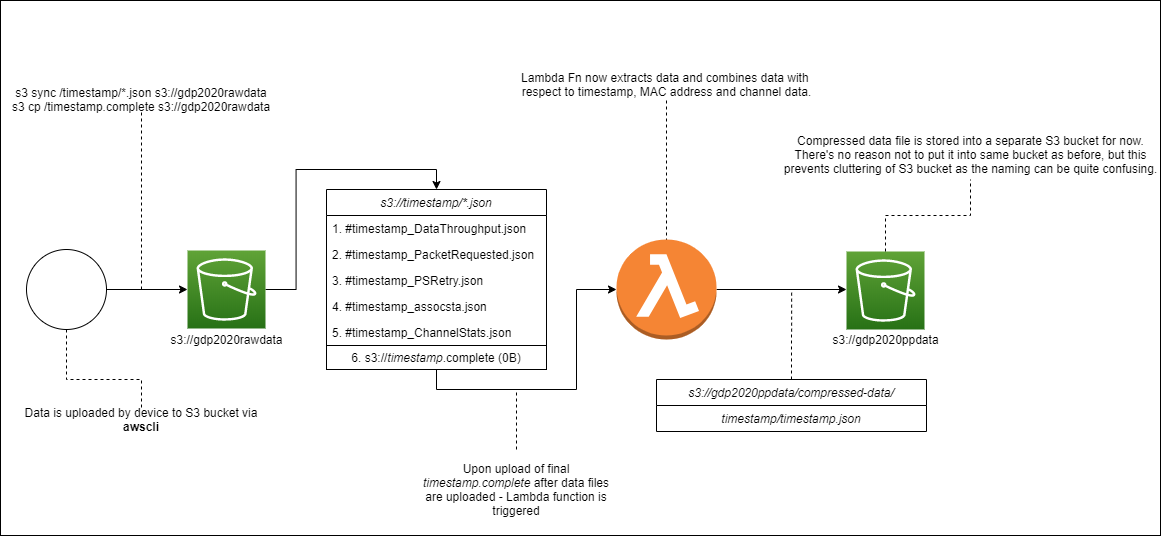
\includegraphics[width=1\linewidth]{pages/Chapter3/Chapter 3 images/S3_to_Lambda_to_S3.png}
    \caption{Triggering Lambda from S3 Uploads - \textit{The full scale diagram can be seen in Appendix E} [\ref{appendix:data_flow_from_laptop_to_cloud}]}
    \label{fig:s3_lambda_s3}
\end{figure}

\subsection{Machine Learning on the Cloud}

The following pipeline shown in \ref{appendix:ML process pipeline} summarizes the machine learning processes that will be carried out.
Firstly, the problem in building the machine learning model was identified from the telemetry data collected from the router. With careful analysis over the parameters collected, data throughput rate is chosen to create a class (target variable) labeled as data throughput strength which will be used to build the machine learning model. Data throughput rate is chosen because it is able to show the amount of data which can be received and sent within a given time span. This enables the prediction of a network performance based on the classification of data throughput strength.

\begin{figure}[ht]
    \centering
    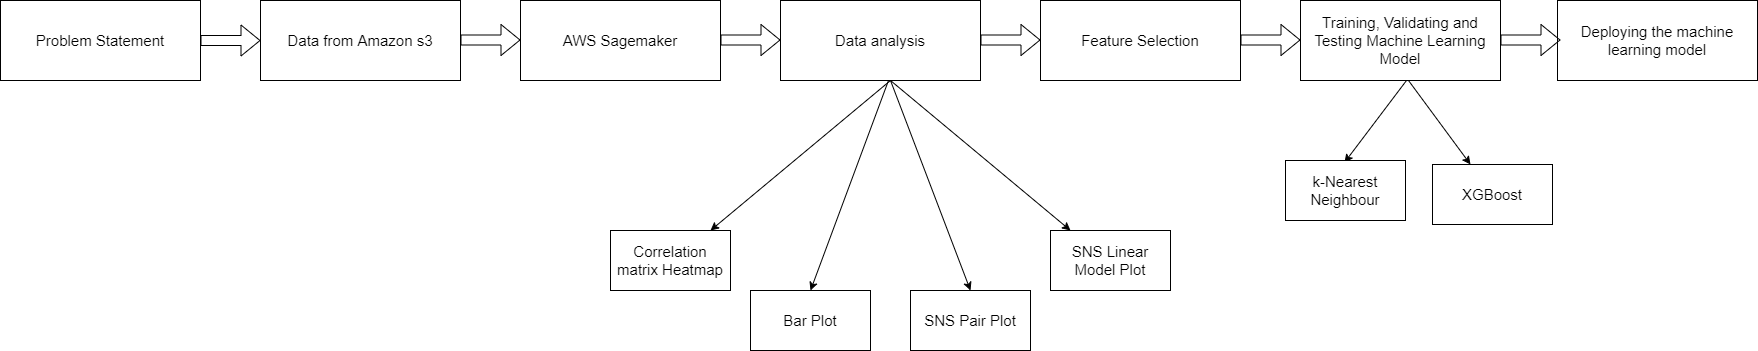
\includegraphics[width=1\linewidth]{pages/Chapter3/Chapter 3 images/Ml.PNG}
    \caption{Machine Learning Process Pipeline - \textit{Full scale diagram is in Appendix B} 
      [\ref{appendix:ML process pipeline}]}
    \label{Machine Learning Process Pipeline}
\end{figure}

The following steps to be carried out are as stated below:
\begin{itemize}
    \item Data stored as JSON files in buckets in the s3 cloud storage is imported into AWS Sagemaker with granted permission access. The code will be written in the Python programming language in JupyterLab. 
    \item Data is analysed using several methods such as correlation matrix, sns pair plots, bar plots and sns linear model plots to find correlation between parameters of the telemetry data.
    \item Useful parameters are extracted and used as features from the data analysis process. 
    \item Features selected are split into a 70:20:10 ratio for training, validating and testing the machine learning model respectively.
    \item Supervised learning algorithms such as XGBoost and k-Nearest Neighbour are used to train the ML model with hyperparameters tuned using the validating set. Testing set is used to evaluate the final performance of the machine learning model.
     \item The performance of the ML model will be evaluated with a confusion matrix with metrics such as accuracy.
    \item The ML model will be deployed after achieving a satisfying performance.
\end{itemize}

The trained machine learning model can be deployed for inference of real-time data. An endpoint will be created automatically once the model is deployed in Sagemaker. The endpoint created for the machine learning model can be invoked in the AWS cloud service.
Using Amazon API Gateway and AWS Lambda services, the endpoint can be invoked to allow the machine learning model to predict new data. To do this, a Lambda function that calls model is first created. An IAM execution role that includes a policy is chosen to give permission access to the Lambda function to invoke the model endpoint. An API gateway will then be created and deployed for the lambda function. This API will trigger an event that invokes the Lambda function where it passes data. Postman, an HTTP client for test service is used for the testing phase of the model endpoint. An invoked URL provided will be entered onto Postman with the data included in it. The prediction results on the data passed into Postman by the ML model will then be displayed on the interface. 



\section{Data Analytics and the Over-the-Top Application}


%     2. ... further chapters discussing system design, build, testing, integration and further testing...







%% ----------------------------------------------------------------
%% Introduction.tex
%% ---------------------------------------------------------------- 
\chapter{Implementation} \label{Chapter:Implementation}



%     3. a chapter introducing final outputs with reference to the original Project Specification (and any revisions to the Project Specification).












\section{Data Collection and Transformation}

This section of the report will further discuss the application of the background research conducted into the extraction of wireless telemetry data (Section \ref{section:WirelessTelemetryResearch}) and the implementation of the system design (Section \ref{data_collection_design}). 
%Akshay to write these sections
\subsection{Data collection from the Router}
\label{Section: Data collection from the Router}

As discussed in previous sections all wireless telemetry data will be collected using the WiFi Radar feature on the ASUS Web GUI. There are multiple approaches to data collection which will be implemented and assessed in order to provide an efficient and non-intrusive method. As shown in Figure \ref{fig_WiFiRadar} the .db file can be downloaded through the ASUS GUI by clicking the "Save Database to File" button. The first two methods will implement data collection using Google Chrome as the main web driver and the final method will use SSH (Secure Shell) in order to access the router OS. 

\subsubsection{Tampermonkey Web Scraper} \label{section:Tampermonkey}

Tampermonkey \cite{tampermonkey} is a Google Chrome browser extension that enables the user to insert and use additional userscripts, which are JavaScript programs, into a web page. The addition of these userscripts allow the user to modify, add and automate functions on a web page. 

With Tampermonkey a userscript is to be created that periodically clicks the "Save Database to File" button. The script is configured to automatically start the data collection process once the specified web page is open (http://router.asus.com/configure.asp) so no additional setup is required. In the implementation of the script the HTML code was inspected to figure out the "input element id" of the buttons. The "Start Data Collection" and "Save Database to File" buttons have the element id's "startbutton" and "exportdbbtn" respectively. Then a function was written to click the "exportdbbtn" button every 5 seconds, which is in line with the lowest sampling interval for the ASUS router data recorder. The .db file is then downloaded into the directory specified in Google Chrome settings under Download Location, where it will go further processing (Section \ref{section:Data Extraction}).

\begin{lstlisting}[language=HTML, caption={Tampermonkey Data Collection Userscript Snippet}, label={lst:tampermonkey}]
(function start() {
    document.getElementById('startbutton').click();
})();

(function() {
    'use strict';
    var button = document.getElementById('exportdbbtn');
    setInterval(function(){
	button.click()
},5000)
})();
\end{lstlisting}




\subsubsection{Selenium WebDriver}

Selenium WebDriver is a web-based automation tool, the Python APIs allows for connection with a web browser of the users choice through which browser-based automation suites and tests can be easily created \cite{selenium}. In this project Selenium will be implemented to automate the data retrieval part of the telemetry pipeline, using the ASUS Web GUI. 

Firstly, the Selenium working environment has to be setup, for this the package and a web-driver must be installed. The Google ChromeDriver web-driver will be the main interface as it provides capabilities for automated testing of webapps, navigation of web pages, JavaScript execution and much more. ChromeDriver version 87.0.4280.88 is used as this is the version associated with the Google Chrome Browser pre-installed on the work station. Then using ChromeDriver, a new window is opened in order to access the desired web page, which in this case is the ASUS router login page (http://router.asus.com/Main\_Login.asp) as shown in Figure \ref{fig:ASUSLoginPage}. From this point the \textit{find\_element\_by\_id()} function is used to identify the username and password elements on the web page in order to login to the router. 

\begin{lstlisting}[language=Python, caption={ASUS Router Login Code Snippet (Selenium)}, label={lst:selenium}]
login_user = driver.find_element_by_id('login_username')
login_user.send_keys(USERNAME)
login_pass = driver.find_element_by_name ('login_passwd')
login_pass.send_keys(PASSWORD)
\end{lstlisting}

\begin{figure}[ht]
    \centering
    
\includegraphics[width=1\linewidth]{pages/Chapter4/Chapter 4 Images/ASUSLoginPage.PNG}
    \caption{ASUS Web GUI Login Page}
    \label{fig:ASUSLoginPage}
\end{figure}

Now having logged into the ASUS router Web GUI, the next stage is to navigate into the Advanced Troubleshooting page (http://router.asus.com/configure.asp), which is where the data collection process is configured and from where the database file is downloaded. Then using the same procedure described in Section \ref{section:Tampermonkey}, the data collection process is started and the "exportdbbtn" is periodically clicked every five seconds using a \textit{while True} forever loop.

This method of data retrieval will automatically launch the ChromeDriver, login to the ASUS router Web GUI, navigate to the data collection configuration page and start the automatic download of the database file every five seconds. 


\subsubsection{Secure Shell (SSH)}

SSH is a network communication protocol that utilises encryption to secure the connection between client and server, allowing network service operations \cite{ssh}. For this project SSH will be used for remote command execution to login and retrieve the database file from the ASUS router. The SSHv2 protocol version is used, and was initially tested using the PuTTY client \cite{putty}. The standard TCP port for SSH is 22 but in the router setting this had to be changed to 1026 as the recommended SSH ports for the ASUS router was 1025 - 65535 due to security concerns. Having now established that it is possible to SSH into the ASUS router, the next step is to find where the database file is stored. Using the command \textit{ls} all directories were searched in order to find the file location of the database, Figure \ref{fig:PuttyAsusFiles} shows a non-exhaustive list of files and directories stored on the ASUS router. Further this, it was found that the database file location was \textit{'/tmp/db/visdata.db'}.

\begin{figure}[ht]
    \centering
    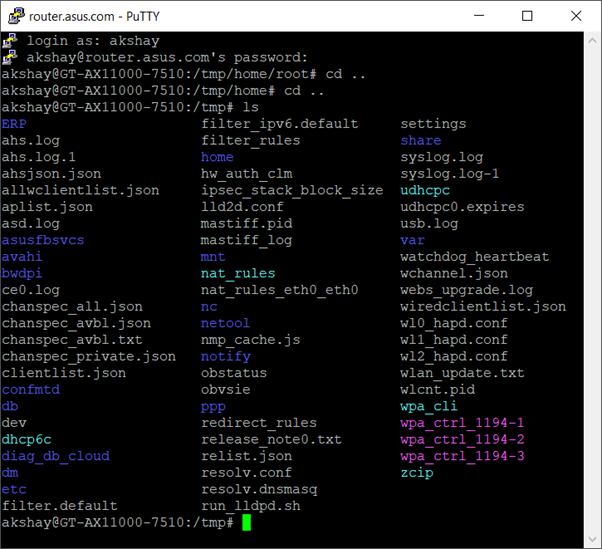
\includegraphics[width=1\linewidth]{pages/Chapter4/Chapter 4 Images/PuttyFiles.png}
    \caption{List of Computer Files on ASUS Router Using PuTTY}
    \label{fig:PuttyAsusFiles}
\end{figure}

Next a Python Script that would run in the background of the laptop connected to the ASUS router, needed to be created. To establish an SSH connection to the router, the package Paramiko \cite{Paramiko} is used as this allows implementation of the SSHv2 protocol for Python.

\begin{lstlisting}[language=Python, caption={Paramiko SSH Client Python Code Snippet}, label={lst:paramiko}]
ssh_client = paramiko.SSHClient()
ssh_client.set_missing_host_key_policy(paramiko.AutoAddPolicy())
ssh_client.connect(host,port,username,password)
\end{lstlisting}

Then the SCP Python module \cite{scp} for Paramiko is used as this enables the transport of files between client and server via the SCP1 protocol. The SCPClient \textit{get.transport()} function is used to retrieve the database file every five seconds once again using a \textit{while True} loop.

\begin{lstlisting}[language=Python, caption={SCP Client Python Code Snippet For Data Retrieval}, label={lst:SCP}]
ssh_client.scp = SCPClient(ssh_client.get_transport())
while True:
    ssh_client.scp.get('/tmp/db/visdata.db', localpath)
    time.sleep(5)
\end{lstlisting}


\subsection{Data Extraction} \label{section:Data Extraction}

Now with the data retrieval section of the telemetry pipeline established, the next stage is to implement the data extraction process from the .db database file. As stated in Section \ref{Section: Data Categorisation} there are many data tables within the database files, a number of which are redundant in the progression of this project. Due to this only the ChannelStats, PacketRequested, Datathroughput, assocsta and PSRetry tables will be converted into the JSON format. 

\subsubsection{Detection of DB File}

With the aim of fully automating the data collection, retrieval and transformation portions of the wireless telemetry pipeline, and further the implementation of the data collection from the router (Section \ref{Section: Data collection from the Router}) there needs to be method for detecting when a new database file is downloaded. Once it has been detected that a new database file has been downloaded into a specified directory, the program should trigger the data transformation functions. 

The implementation of this automatic file detection is conducted using the Watchdog Python API library which allows the system to monitor for file system events \cite{watchdog}. The process of creating a file system monitor to detect changes in a directory is as follows. First, a handler instance of the \textit{watchdog.observers.Observer} thread class is created. Then, a subclass of the \textit{watchdog.events.FileSystemEventHandler} is created. Next, the directory path to be monitored is set and scheduled using the event handler attached to the observer instance. Finally, the observer thread is started where it will wait an event to trigger further processes. 

\begin{lstlisting}[language=Python, caption={Watchdog File System Event Handler Code Snippet}, label={lst:watchodog}]
class Handler(FileSystemEventHandler):
    @staticmethod
    def on_any_event(event):
        if event.is_directory:
            return None

        elif event.event_type == 'created':
            print ("Received created event - %s.")
            time.sleep(5)
            fileAdded()

        elif event.event_type == 'modified':
            print ("Received modified event - %s.")
\end{lstlisting}

As shown in the listing above when a new file is added to the directory being monitored, the funtion \textit{fileAdded()} is called. In this function the name of the latest file to be added is obtained using the Python modules glob and os. 

\begin{lstlisting}[language=Python, caption={Getting The Latest File Name Code Snippet}, label={lst:latestFile}]
def getLatestFileName():
    list_of_files = glob.glob('C:/Users/.../*.db')
    latest_file = max(list_of_files, key=os.path.getctime)
    return latest_file
\end{lstlisting}

Now having detected that a new database file has been downloaded, and with the name of the new file obtained, further data transformation process can be executed. 

\subsubsection{Data Extraction from DB File}

For the automation of the data extraction process a Python script is created that will open and read all relevant data in the .db file, then it will convert the data into Python objects and finally serialise these objects into the JSON format. 

In order to open and read in the .db file in Python the SQLite3 library is used, because it allows for access into databases that use nonstandard variants of the SQL query language \cite{sqlite3}. Firstly, a \textit{Connection object} is created to establish a connection to the SQLite database, where the object will represent the database \cite{sqlitePython1}. 

\begin{lstlisting}[language=Python, caption={SQLite3 Database Connection Object Code Snippet}, label={lst:Connection Object}]
def create_connection(db_file): 
    conn = None
    try:
        conn = sqlite3.connect(db_file) 
        return conn
    except Error as e:
        print(e)
    
    return conn
\end{lstlisting}

Having established the database connection, a cursor object is created (\textit{conn.cursor()}) so that its \textit{execute()} method can be called to perform SQL commands. Then a \textit{SELECT} statement is executed so as to access the data inside a specified datatable. Next, the method \textit{fetchall()} of the cursor object is called in order to retrieve all the data inside a datatable. 

\begin{lstlisting}[language=Python, caption={SQLite3 Cursor Object and Its Execute and Fetchall Method Code Snippet}, label={lst:Cursor Object}]
cur = conn.cursor()
cur.execute("SELECT *FROM RxCRSGlitches")
rows = cur.fetchall()
\end{lstlisting}

With the .db database file now opened and with the ability to read data from it, the next step is to convert the datasets into Python Objects. For this each row in the datatable is temporarily stored into a tuple, which then gets appended into an array and this process is repeated for all rows in the table. Then, the Python object is serialised and converted into a JSON string using the \textit{json.dumps()} function. The \textit{dumps()} function is used rather than \textit{dump()} because the later writes Python serialised objects directly into a file, whereas the other encodes the object into a JSON formatted string. After this, the JSON formatted string is written into an outfile and saved into a specific directory to undergo further processing if required or to be directly uploaded onto the S3 Bucket. This process above is repeated and performed for every datatable that needs to be converted. 

Due to the fact that new datasets are appended to the .db database file even after downloading the latest version, in order to only have the latest timestamps and to avoid the use of very large JSON files a timestamp limit needs to be introduced. This is simply achieved using an if statement with a global cut off timestamp variable on the last datatable converted. 

\begin{lstlisting}[language=Python, caption={JSON Conversion Code Snippet}, label={lst:conversion example}]
rowarray_listassocsta = []
for row in rows:
    if row[1] > cutOffTimestamp:
        lastTimestamp = row[1]
        tupleassocsta = (row[0], row[1], row[2], row[3], row[4])
        rowarray_listassocsta.append(tupleassocsta)
            
stringassocsta = json.dumps(rowarray_listassocsta)

with open('C:/Users/...', 'w') as outfile:
    outfile.write(stringassocsta)
\end{lstlisting}

%Anurag here
\subsubsection{Data Compression of JSON Files}
\label{data_compression}
Once the data has been split up into five different JSON files after each relevant datatable has been extracted. The Python script in charge of compression works as shown by the block diagram in Figure \ref{fig:json_compression}. JSON files are retrieved and compressed into one JSON file for easier processing and transportation, while also removing any unnecessary data. It does this by retrieving each JSON file, generating a list of available MAC Addresses and for each one, iterating through the data tables for one time stamp.
\begin{figure}[ht]
    \centering
    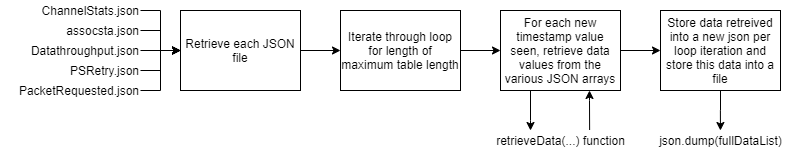
\includegraphics[width=1\linewidth]{pages/Chapter4/Chapter 4 Images/json_compression.png}
    \caption{Block Level Diagram of Compression Transformation of JSON Datafiles}
    \label{fig:json_compression}
\end{figure}
The diagram in Figure \ref{fig:data_table_data} shows what data can be retrieved from within each data table and how it appears within the new compressed JSON file. Only the most relevant and usable data is retrieved from each table, otherwise it removed.
\begin{figure}[ht]
    \centering
    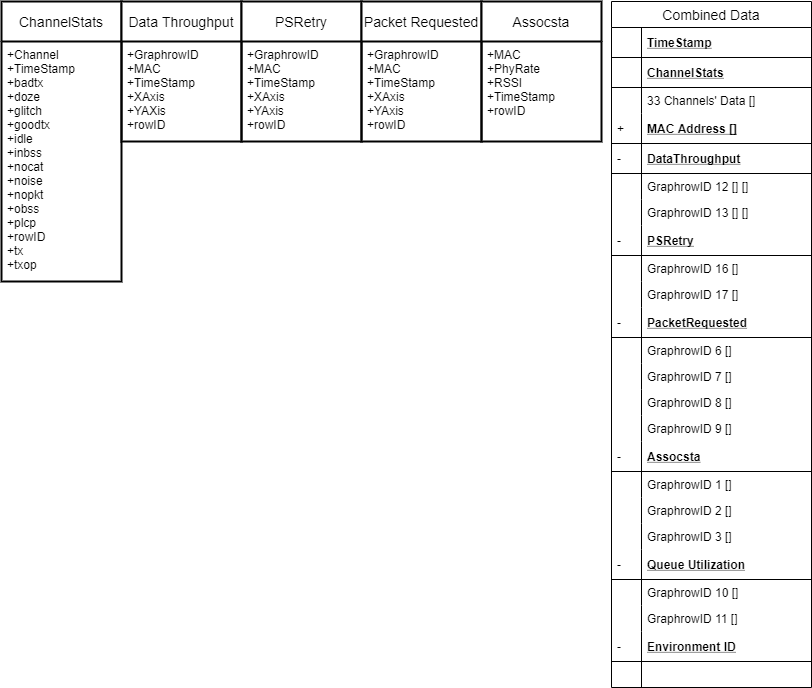
\includegraphics[width=1\linewidth]{pages/Chapter4/Chapter 4 Images/router_data-Dataset Contains.png}
    \caption{Relevant Data within each Data Table}
    \label{fig:data_table_data}
\end{figure}


\subsection{Telemetry Pipeline 1/3 - Upload to Cloud Directly} \label{Section:pipeline1/3}
The first pipeline method to be implemented is for the data to be taken from the laptop directly to the cloud. In this route an API Gateway is setup on the cloud as described in Section \ref{api_gateway_design}
and data can be sent to it and stored securely to an S3 bucket for pre-processing. The API Gateway follows the RESTful framework described in \ref{fig:api_gateway_methods}
%DON@T FORGET TO FINISH REFERENCE HERE TO API GATEWAY IMPL. SECTIOn



Using the Put method under the URL \textit{s3://gdp2020rawdata/\{timestamp\}/\{item\}} allows us to place the individual JSON files into the raw data bucket. Once all 5 JSON files are uploaded under the names:
\begin{itemize}
    \item \{timestamp\}\_PSRetry.json
    \item \{timestamp\}\_PacketRequested.json
    \item \{timestamp\}\_ChannelStats.json
    \item \{timestamp\}\_assocsta.json
    \item \{timestamp\}\_Datathroughput.json
\end{itemize}
Then an empty file is also uploaded to the cloud that also follows this pattern,\\ 
\textit{\{timestamp\}.complete}, which will trigger the pre-processing Lambda function. This process was previously described in \ref{cloud_lambda}. Once the Lambda function is triggered by the .complete file, it will begin its operation as described above in Section \ref{data_compression} and will store the pre-processed data or \textit{compressed} data into the S3 Bucket as \\\textit{s3://gdp2020ppdata/compresseddata/\{timestamp\}.json}.

Using the Python \textit{requests} package \cite{python_requests_lib}, one can begin to upload as necessary using the following parameters:
\begin{itemize}
    \item \textbf{Payload}: json.dumps(JSON object)
    \item \textbf{Headers}:\begin{itemize}
        \item \textit{Content-Type}
        \item \textit{Host}
        \item \textit{Authorisation}
        \item \textit{Content-Length}
        \item \textit{Content-Type}
    \end{itemize}
\end{itemize}
After the requests payload is defined with the correct headers, using the following function in Listing \ref{lst:request_code} and storing the response, one can view the status code and use it to confirm correct upload. This follows standard HTTP status code guidelines, with a response of 200 being correct operation and other response code illustrating that something went wrong.
\begin{lstlisting}[language=Python, caption={Requests Library Usage}, label={lst:request_code}]
response = requests.request("PUT", url=payload, headers=headers)
print(response.status_code)
print(response.text)
\end{lstlisting}

\subsubsection{Laptop-to-Cloud Direct Upload Timings}

In order to directly compare the timings for the three different pipelines, the direct upload method has to be timed. This timing operation is broken down into three sections, time it takes to retrieve the database file, time to convert db file into the five separate JSON files and finally the time to upload the individual JSON files to the cloud storage. For this the Python time module is used with its \textit{time.time()} function implemented to record the start and end time of each operation. Then these time values are outputted onto a JSON file and placed in the shared directory of the edge node so it can be displayed in the web application for direct comparison. 

\begin{lstlisting}[language=Python, caption={Laptop-to-Cloud Timing Code Snippet},
label={lst:ltc code}]
jsonTimings = { 	"loadDB": loadTime,
                        "Extract": convertTime,
                        "uploadJSONs": uploadTime,
                        "totalTime": loadTime + convertTime + uploadTime
                  }
    
    stringjsonTimings = json.dumps(jsonTimings)

    with open ('C:/Users/.../timing.json', 'w') as outfile:
        outfile.write(stringjsonTimings)
\end{lstlisting}







\section{Localised Processing, Storage and Classification}
In this section the report will discuss the implementation of the edge node and all facilities within it.
\subsection{Setting up the Environment}
In order to simulate an edge Device rather than a separate piece of hardware, a Virtual Machine (VM) can be setup on the laptop. However, the virtual machine is just to represent an edge device running an embedded UNIX OS. In this scenario using Vagrant in conjunction with VirtualBox allows for the setup and use of a virtual Ubuntu system. This is all to emulate an edge device such as a Raspberry Pi or a server running at the remote location. The guide on the Vagrant website takes the developer step by step through the stages of getting the VM setup. \cite{installing_vagrant}. 

Once this is setup, the Greengrass Core (GGC) can now be initiated and ran on the \textit{Edge Device}. First the Greengrass group was created via the IoT Core page on AWS and then a group was setup using the default settings. When the group is first initialised, a zip file filled with correct certifications and configuration files is produced. These files must be placed into the installed GGC folder on the Edge Device under \textit{/greengrass/certs} and \textit{/greengrass/config}. Then the Greengrass Core can be started up by running the program stored at \textit{/greengrass/ggc/core/greengrassd}. Upon doing this, the message shown in Figure \ref{fig:running_greengrass_on_vm} will appear showing that the Greengrass Core has successfully launched and deployments will then begin running. 

\begin{figure}[ht]
    \centering
    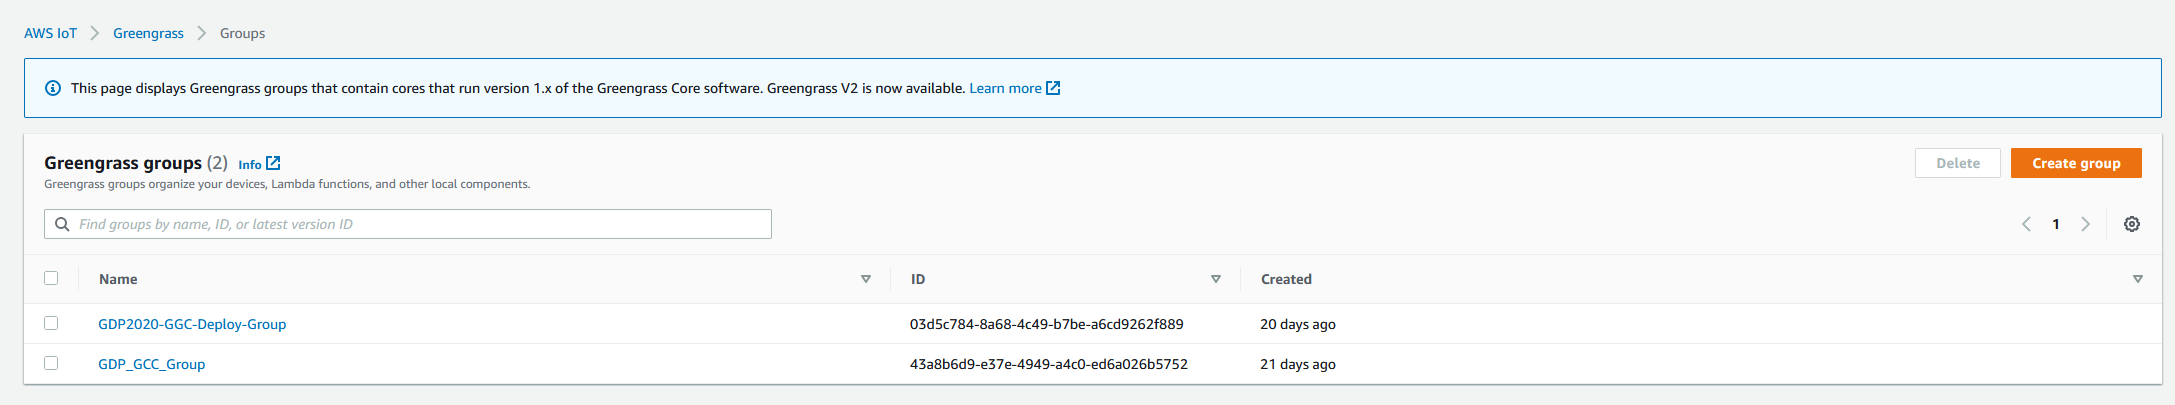
\includegraphics[width=1\linewidth]{pages/Chapter4/Chapter 4 Images/greengrass_group.png}
    \caption{Setting up Greengrass Group on the AWS IoT Core dashboard}
    \label{fig:my_label}
\end{figure}
\begin{figure}[ht]
    \centering
    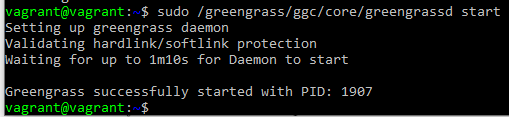
\includegraphics{pages/Chapter4/Chapter 4 Images/correctly_starting_greengrass.png}
    \caption{Deploying and Running Greengrass on the VM}
    \label{fig:running_greengrass_on_vm}
\end{figure}

There are then some additional steps that need to be run for installing the pre-requisites and give the Greengrass Group, access to run its runtime and the Greengrass daemon. The pre-requisites are specifically the Lambda run-times required (e.g. for Python or NodeJS). These instructions and the specific commands can be found in the AWS Documentation in Greengrass Deployment \cite{greengrass_deployment}.

\subsection{Attaching Lambda Functions to the Greengrass Group}
Once the Greengrass Group is established, a Lambda function to run on the device can be setup as long as the runtime requirements are also on the device (e.g. nodejs12.x must be installed to run NodeJS at the edge device). Then on the Greengrass Group dashboard a new existing Lambda function is attached, as shown in Figure \ref{fig:adding_new_lambda_to_ggc}. The first step is to add the Lambda function, then attach an existing Lambda function from the provided list. This Lambda function must already have been created in the AWS Lambda Dashboard.

\begin{figure}[ht]
    \centering
    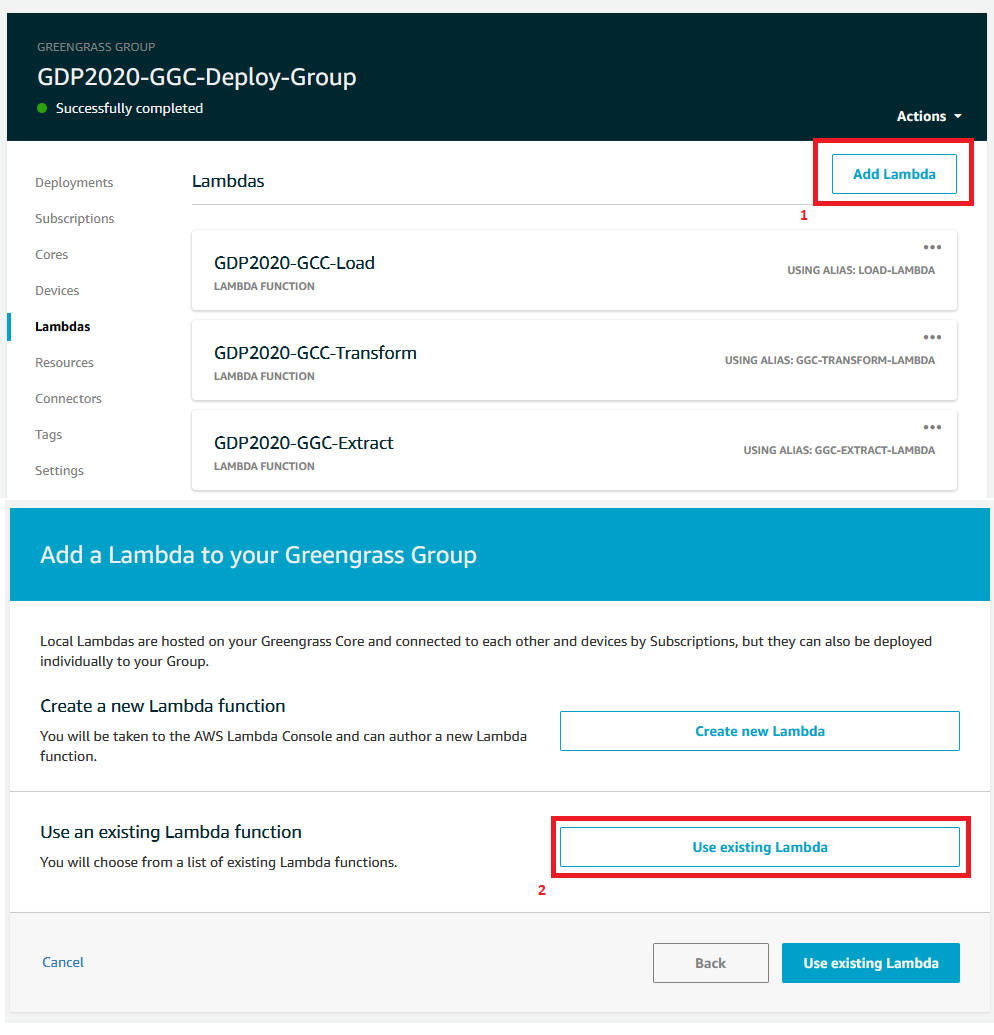
\includegraphics[width=0.7\linewidth]{pages/Chapter4/Chapter 4 Images/greengrass_new_lambda.png}
    \caption{Adding a new Lambda Function via the Dashboard.}
    \label{fig:adding_new_lambda_to_ggc}
\end{figure}

Once this is complete, the drop down in the top right of the Greengrass Groups dashboard allows you to deploy or re-deploy an existing version, as shown in Figure \ref{fig:deploy_on_dashboard}.

\begin{figure}[ht]
    \centering
    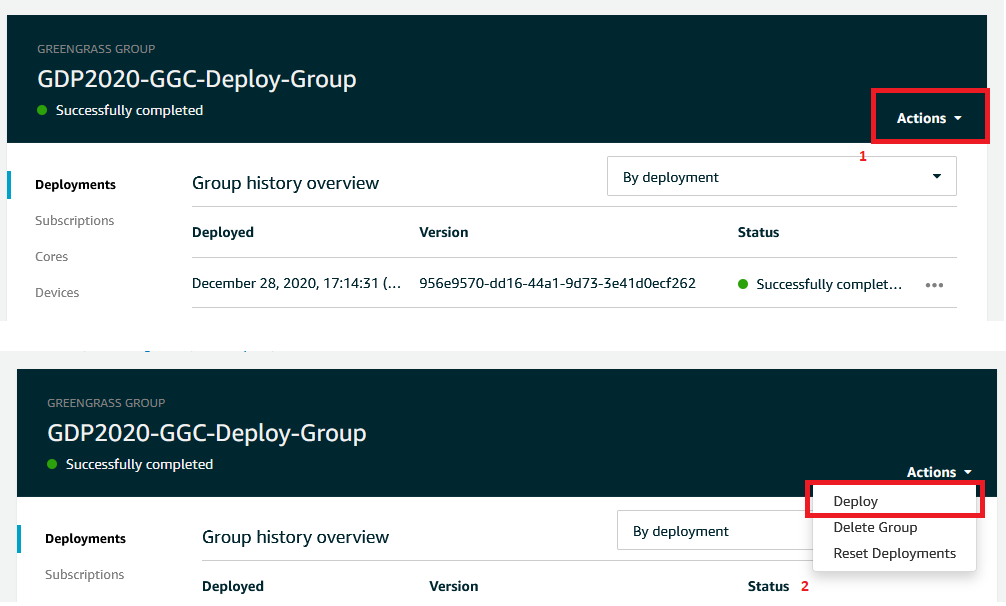
\includegraphics[width=0.7\linewidth]{pages/Chapter4/Chapter 4 Images/deploy_group.png}
    \caption{How to deploy the Greengrass Group via the Dashboard}
    \label{fig:deploy_on_dashboard}
\end{figure}


To enable the GGC to access the hosts' local resources, \textit{Local Resource Access} must be setup on the group. Local Resource Access is a way for the containerised Greengrass Core to gain access securely to a specific directory outside of the container. This is done by setting up a \textit{src} directory on the host, and a matching \textit{dest} directory on the Greengrass device. This process can be seen in Appendix \ref{appendix:ggc_lra}. A folder within the containerised GGC is labelled as \textit{'dest/LRAtest/...'} and outside of the container on the host device (or VM for this project) is a similar folder \textit{'src/LRAtest/...'}. These two directories are linked with each other. Files stored into the former location will be also seen on the host machine under the latter location and visa versa.

The next following sections will discuss how to setup each Lambda function.
\begin{itemize}
    \item Extract - \ref{extract_fn_impl}
    \item Transform - \ref{transform_fn_impl}
    \item Load - \ref{load_fn_impl}
    \item Local ML Inference - \ref{load-ml-fn}
    \item Remote ML Inference - \ref{remote-ml-fn}
    \item NodeJS Web Server Application - \ref{nodejs-server}
\end{itemize}


\subsection{Extract Function}
\label{extract_fn_impl}
The first localised Lambda function, the Extract function, collects any .db files from the End-user's device and begins processing it at the Edge. This frees up the End-user's device for other tasks as previously explained. As this is the first documentation of Lambda Function implementation, one requirement to run any function is to include the Greengrass SDK. This is done by uploading a zip file to the Lambda function which includes the main program file and the SDK Folder as seen in Figure \ref{fig:ggc_sdk_inclusion}
\begin{figure}[ht]
    \centering
    
\includegraphics{pages/Chapter4/Chapter 4 Images/LambdaFns/ggc_sdk_inclusion.png}
    \caption{How the zipped  directory needs to be uploaded.}
    \label{fig:ggc_sdk_inclusion}
\end{figure}

This setup must be completed for each function, and any external Python dependencies must also be included in this zip file. Once the setup is complete, then the Python application can be developed. The extract-function Python implementation follows the data-flow shown in Figure \ref{fig:lambda_extract_fn}.

\begin{figure}[ht]
    \centering
    
\includegraphics[width=1\linewidth]{pages/Chapter4/Chapter 4 Images/LambdaFns/extract-fn.png}
    \caption{Extract Lambda Function Block Diagram}
    \label{fig:lambda_extract_fn}
\end{figure}

The implementation for this function is very similar to the implementation for the Laptop-To-Cloud pipeline with the main changes being the setup required for the local resource access from the edge node.

\subsection{Transform Function}
\label{transform_fn_impl}
The transform function implementation follows the block diagram shown in Figure \ref{fig:lambda_transform_fn}, with the main points being where the output file and the compressed JSON object with all the separate data tables' data in one is placed. The output file is placed into three locations for usage by other Lambdas. It should be noted that it was chosen to replicate the three output files so as to avoid any issues with access from multiple locations (separate Lambda functions). However, this leads to a longer run-time as the write operation has to be run three times rather than once, but is only a problem for very large files as is seen later in the testing stages.

\begin{figure}[ht]
    \centering
    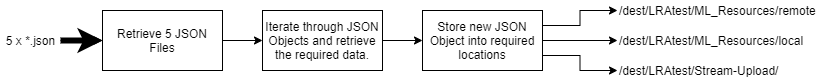
\includegraphics[width=1\linewidth]{pages/Chapter4/Chapter 4 Images/LambdaFns/transform-fn.png}
    \caption{Block Diagram of Transform Function at the Edge Node}
    \label{fig:lambda_transform_fn}
\end{figure}


\subsection{Load Function}
\label{load_fn_impl}
For this Lambda function, the Python library \textit{requests} is used and so the dependency folder must be extracted from several ways. 
\begin{itemize}
    \item Copy directly from developer's Python dependencies list.
    \item Setup a virtual environment for Python and install all dependencies, this will then be stored locally in that virtual environment. These can then be zipped up and extracted and the developer's program injected into the zipped folder for upload to the Lambda function.
\end{itemize}

The requests library is small with no build requirement (this will become an issue later for the XGBoost library). The required directory was copied directly from the developer's Python-libraries list after using \textit{pip install requests} and \textit{pip show requests} to ensure no other sub-dependencies were required. The latter command also showing where this installed requests library can be found so as to be copied. The final zipped folder to upload to the Load-Lambda function is shown in Figure \ref{fig:lambda_requests_ggc_sdk}.

\begin{figure}[ht]
    \centering
    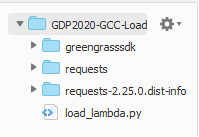
\includegraphics{pages/Chapter4/Chapter 4 Images/LambdaFns/ggc_sdk_requests_inclusion.png}
    \caption{File structure for Upload to Load Lambda with Requests and GGC SDK}
    \label{fig:lambda_requests_ggc_sdk}
\end{figure}

The implementation of the load Lambda function follows the block diagram in Figure \ref{fig:lambda_load_fn}. Environment variables can also be setup within the AWS Lambda dashboard to ensure no details of the private key are released without intention. 

\begin{figure}[ht]
    \centering
    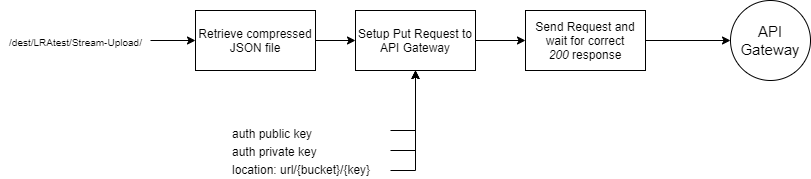
\includegraphics[width=1\linewidth]{pages/Chapter4/Chapter 4 Images/LambdaFns/load-fn.png}
    \caption{Block Diagram of Load Function at the Edge Node}
    \label{fig:lambda_load_fn}
\end{figure}


\subsection{Local-ML Function}
\label{load-ml-fn}
%looooooooooooong%
For the Local-ML Lambda function setup there are several steps that need to be completed. \begin{enumerate}
    \item Import the Sagemaker Model from either Sagemaker or S3.
    \item Setup Python Dependencies for use of XGBoost Python Library at the edge, these must be built specifically for the end-device architecture and OS. (e.g. Linux on x84\_64 architecture).
    \item Upload zipped file of Dependencies and Python program file.
    \item Complete program and deploy to Greengrass Core.
\end{enumerate}
These four stages describe the implementation process, with the second stage being the most difficult and time consuming. This is because the XGBoost Python package and its sub-dependencies must be built from source due to usage of C program files within XGBoost, and these must be built for the target device. 



The first stage of this setup procedure is as follows. In the development stages of Sagemaker Model Training and Deployment, a model is produced as a zip file. This zip file containing the ML-Model can be imported direclty into the Greengrass Group as a resource to be used within the container environment. It can be either imported from S3 or directly from Sagemaker. This is seen in Figure \ref{fig:ggc_model_import} where the ML model must also be attached to a Lambda function for it to be accessible by that Edge-based Lambda function. First the \textit{'Add machine learning resource'} must be clicked, then the model name entered and a choice must then be made for the source location of the model. As shown in Figure \ref{fig:ggc_model_import}, the model is uploaded from a provided S3 bucket and location within it. Then the local path within the Greengrass container is also chosen. This is for usage within the attached Lamda function to the Machine Learning Resource, to open the directory with the model.

\begin{figure}[ht]
    \centering
    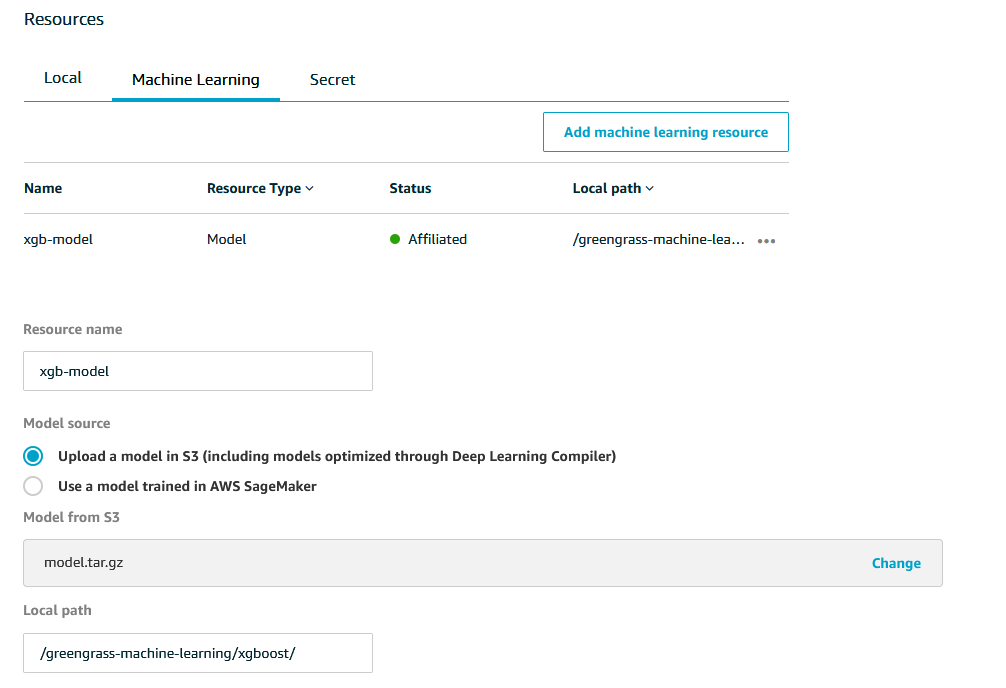
\includegraphics[width=1\linewidth]{pages/Chapter4/Chapter 4 Images/LambdaFns/xgboost_model_import_ggc.png}
    \caption{Importing XGBoost Model from S3 into the Greengrass Group as a local Resource}
    \label{fig:ggc_model_import}
\end{figure}

Once the ML-Model is attached and a Lambda function to handle the Local-ML Inference is also attached, then the dependencies can be built. First an EC2 instance is instantiated in order to help the developer build and pack the dependencies. The developer must set up a \textit{virtual Python environment} so that the Python dependencies are installed remotely and any sub-dependencies are also present (as these must also be zipped as previously mentioned). The developer must then also install Python 3.7 rather than Python 3.8 within the Virtual environment as Greengrass at the time of writing this report only supports Lambda functions with a runtime of Python 3.7. Once the \textit{virtual Python environment} is setup and any sub-depencies or other required libraries are also installed within. In this case, the dependencies required are:
\begin{itemize}
    % \item \textit{xgboost}
    \item \textit{numpy}
    \item \textit{scipy}
    \item \textit{six}
    \item \textit{pkg\_resources}
\end{itemize}
Once these dependencies are setup, download the XGBoost source files from GitHub and use CMake to manually compile the program for the Amazon Linux OS running on x86\_64 architecture. It should be noted that CMake will also need to be downloaded and compiled from scratch. The exact commands to achieve this can be found on a post by Lucas Silva \cite{silva_2019}. However, these commands must be adjusted for this project's specific sub-dependencies, and the article uses Python 3.8 rather than 3.7, to install Python 3.7 it requires further adjustment of the commands as seen in the article by Rahul Kumar for installing Python 3.7 on Amazon Linux. \cite{kumar_2020} 

Following the instructions provided produces a zip file that can be uploaded to an S3 bucket for retrieval from the EC2 instance and then uploaded into Lambda. Once this is complete the implementation of the program can begin. The implementation of the main program follows the block diagram shown in Figure \ref{fig:localml-function}. The block diagram shows how the program running in the Lambda function will operate. First it must retrieve the model and the JSON file from the appropriate local directories in the Greengrass container. Then apply some pre-processing to make them fit for usage. The XGBoost Python package then comes with a predict function that allows us to input the data parameters for one timestamp and per MAC Address. This output result can then be stored locally, passed to the OTT Application or to the Web server application for live-viewing of the results, as well as for comparisons to the Remote-ML timings.

\begin{figure}[ht]
    \centering
    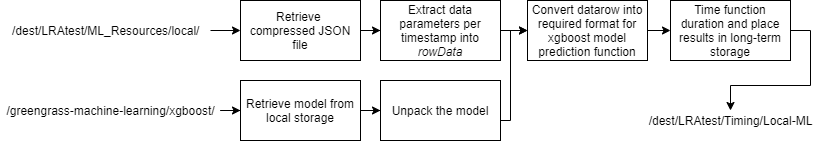
\includegraphics[width=1\linewidth]{pages/Chapter4/Chapter 4 Images/LambdaFns/localml-fn.png}
    \caption{Block Diagram for Local-ML Function at the Edge Node}
    \label{fig:localml-function}
\end{figure}
%Import of Sagemaker model into greengrass via dashboard
%How it can be accessed
%Setup of Dependencies using Cloud-Based resources, ensure version for python3.7, ensuring also size of lambda zip is less than 250mb as a hard limit from them
% any more than 50mb must be uploaded from s3

\subsection{Remote-ML Function}
\label{remote-ml-fn}
Once the requests library is correctly packed with the Lambda program file. As well as the API Gateway setup to trigger a Lambda function, which in turn will trigger the Sagemaker Endpoint. A similar implementation as seen in Figure \ref{fig:lambda_load_fn} is used, however the URL used in the HTTP request will be different. The response from the endpoint is also how the Lambda function will receive the results of the Machine Learning Model's output. A code snippet shows how the request can be setup by reading the JSON file and then sending the data as requested to the API Gateway to be processed by the Cloud-Based Lambda as shown in Listing \ref{lst:edge_remote_ml}
\begin{lstlisting}[language=Python, caption={Sending Data to API Gateway to Invoke Cloud-Based Lambda for Sagemaker Endpoint}, label={lst:edge_remote_ml}]
with open(jsonLoc, 'r') as jF:
                payload = json.dumps(json.loads(jF.read()), separators=(',',':'))
            client.publish(
                topic='mlEndpoint/checkFile', 
                queueFullPolicy='AllOrException', 
                payload="Opened file success!")
            headers = {
                'Content-Type': "application/json, text/plain",
                'Host':"vnl7ji5sz2.execute-api.eu-west-2.amazonaws.com",
                }
            start = time.time()
            response = requests.request(
                                    "POST", url, 
                                    data=payload, 
                                    headers=headers
                                    )

\end{lstlisting}
The implementation for the Cloud-Based Lambda which is responsible for further pre-processing to fit the model is shown in the later section for implementation of Cloud-Based services. The Cloud-Based Lambda interacting with the Sagemaker endpoint will then return the result of the classification in the form of a value of 0 to 4, corresponding to a classification of the data throughput as discussed in the Machine-Learning system design section.


\subsection{Laptop-to-Cloud Pipeline Data Collection}
In order to collect the timing data and transmit it to the Web Server, first the ETL script that runs on the Laptop for the pipeline collects all data and produces a JSON file that contains the data. This data file is stored in the shared network folder for the Edge Node's Lambda function to collect. Upon collection, it will send an MQTT package containing this data to the Web Server for viewing and comparisons to be made.

\subsection{MQTT to Web Application and IoT Cloud}
The primary method for communication from the edge node to the cloud, and from service to service at the edge node is via transportation of MQTT packets. For the most part, the messaging system has been abstracted away so only a subscription topic is used and the data object to be transported. Each service can subscribe to a topic which allows it to listen and be triggered by the new packet or allows the service to successfully publish to the topic.

This means it can be used for debugging as well as real-time application usage. These messages are a clean way to send small data items that cannot be intercepted from outside of the containerised Greengrass Core, hence the usage within this system. The first set of subscriptions to be used is the debugging layer and error checking. During implementation of each Lambda function above, subscriptions and messages were sent to monitor progress of the Lambda function in any of the retrieving, processing or storing stages inside each Lambda function. The debugging subscriptions can be seen in Figure \ref{fig:cloud_mqqt_layer}. In this diagram, each Lambda function that is attached to the Greengrass Group as well as the topic it is subscribed onto.

\begin{figure}[ht]
    \centering
    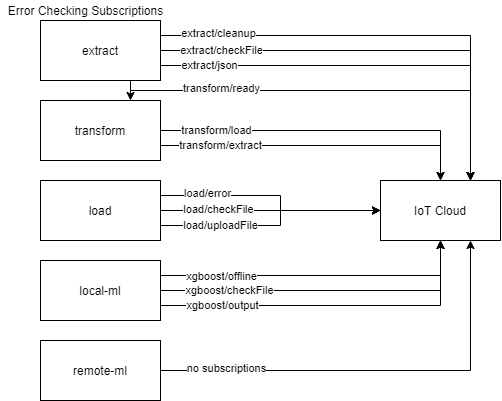
\includegraphics[width=0.75\linewidth]{pages/Chapter4/Chapter 4 Images/LambdaFns/iot_cloud_mqqt.png}
    \caption{Subscriptions from Lambda to IoT Cloud Service for Debugging and Error Checking}
    \label{fig:cloud_mqqt_layer}
\end{figure}

Once the subscriptions have been setup within the Greengrass group as shown in Figure \ref{fig:setup_subs}. It shows the \textit{src} and \textit{dest} addresses for the subscription topic. Any publishes made by the Extract Lambda function will be seen by the IoT Cloud for testing and is discussed further in the testing section.

\begin{figure}[ht]
    \centering
    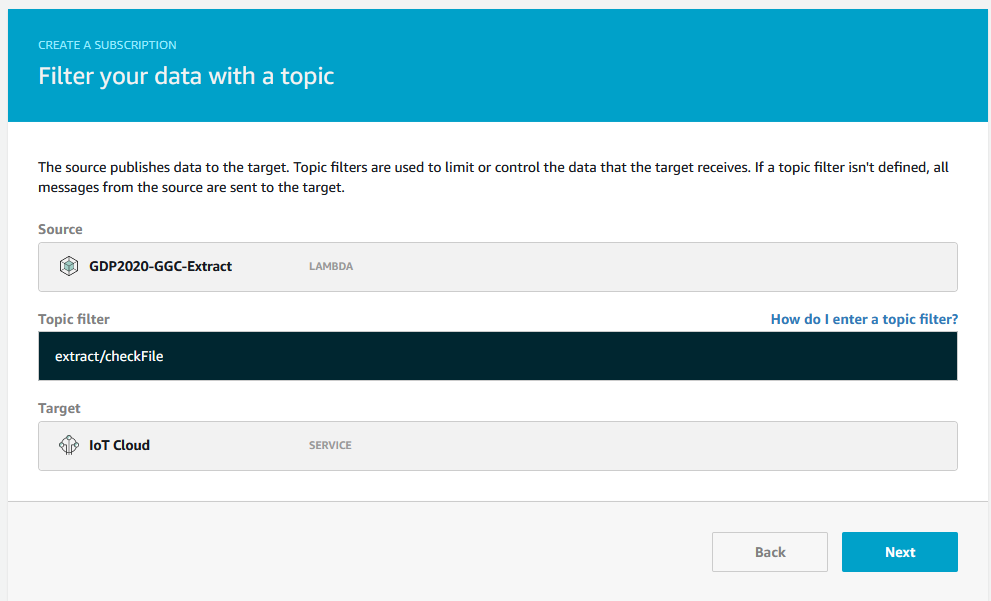
\includegraphics[width=0.75\linewidth]{pages/Chapter4/Chapter 4 Images/setting_up_subscription.png}
    \caption{How the 'extract/checkFile' subscription was setup to send data from the Extract Lambda to IoT Cloud.}
    \label{fig:setup_subs}
\end{figure}

Messages being sent to the IoT Cloud can be seen via the 'Test' tab in the IoT Core dashboard. First the topic to be observed must be entered into the text-box labeled \textit{Subscription Topic}, then the \textit{Display payloads as strings} option should be selected under \textit{MQTT payload display}. Error messages from the Python script can also be captured using \textit{Try} and \textit{Except} blocks to catch and then send any exceptions to the IoT Cloud for easy debugging. This setup is seen in Figure \ref{fig:mqqt_testing_setup}.

\begin{figure}[ht]
    \centering
    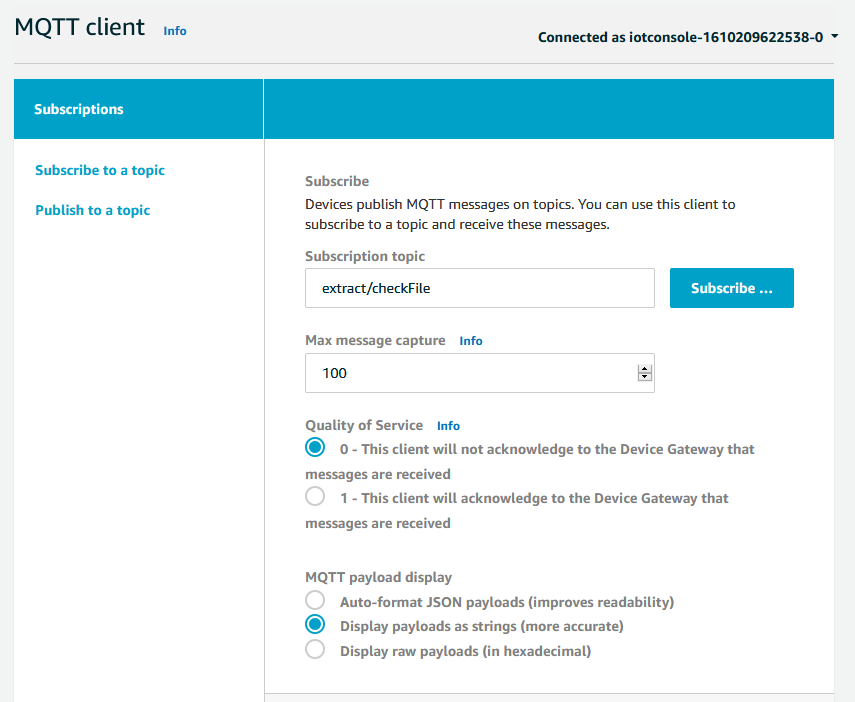
\includegraphics[width=0.75\linewidth]{pages/Chapter4/Chapter 4 Images/setting_up_mqqt_for_test.png}
    \caption{How MQTT Packages can be setup for testing}
    \label{fig:mqqt_testing_setup}
\end{figure}


The above subscriptions were only used for debugging. To send real-time data to the Web-Server application, the subscriptions and topics seen in Figure \ref{fig:mqqt_to_web_app} were setup.

\begin{figure}[ht]
    \centering
    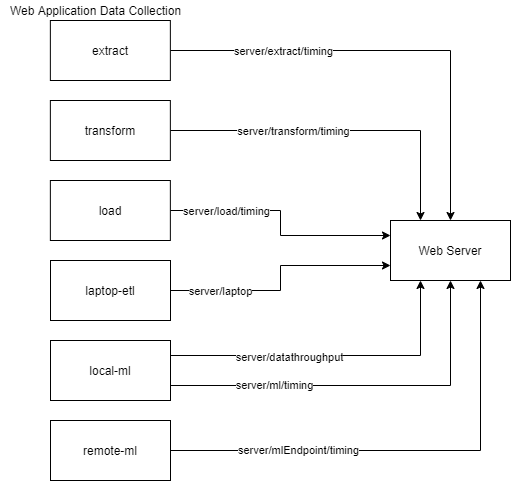
\includegraphics[width=0.7\linewidth]{pages/Chapter4/Chapter 4 Images/nodejs_mqqt.png}
    \caption{Subscriptions and Topics to send data to the Web Application}
    \label{fig:mqqt_to_web_app}
\end{figure}

\subsection{Web Server Application for Live Data Viewing}
\label{nodejs-server}
For this Lambda function, Nodejs is used. Specifically Nodejs 12.x must be used as required by the current version of Greengrass used at the time of this project therefore the runtime must be installed on the edge-device. This is simply a case of downloading the nodejs12.x runtime and storing it on the Edge Devices' \textit{usr/bin/} directory under \textit{nodejs12.x}. This procedure is part of the official documentation regarding Node JS Lambda functions and can be found in more detail on the GitHub page \cite{aws_greengrass_nodejs12_ghub}.

Once this is setup, it is possible to use NodeJS Lambda functions in the Greengrass Group. For the web application, the design choices which needed to be implemented are shown in Figure \ref{fig:web_app_design}. From this, it is understood how each section must be laid out on the Web Server. The central piece will contain a graph to show the data throughput values. Timing of each Lambda function and functions within them will also be shown on the right hand-side of the graph. Then a table with data parameters and classification of the data using the ML model will be shown at the bottom. New data will always be pushed to the top of the table with a maximum of 10 items, so the last table item must be removed.

\begin{figure}[ht]
    \centering
    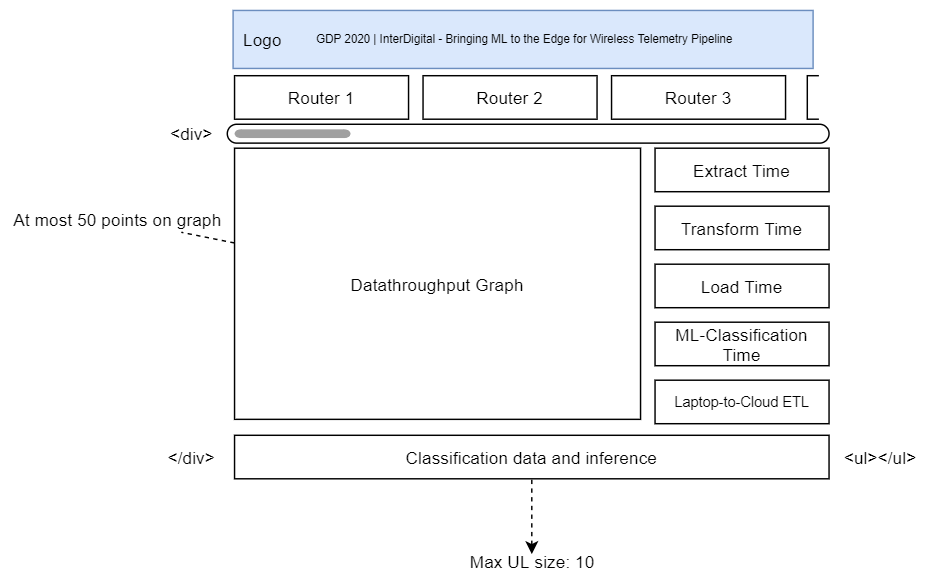
\includegraphics[width=1\linewidth]{pages/Chapter4/Chapter 4 Images/web_app_design.png}
    \caption{Design to be Implemented For Web Application}
    \label{fig:web_app_design}
\end{figure}

In order to set this up, first the back-end of the server must be developed. Using NodeJS for the back-end and Bootstrap \cite{mark_otto_2021}, a HTML/CSS/Javascript package that allows easy website UI/UX elements to be generated can be used to develop the front-end. 

As per all the Lambda functions, anytime a message via a subscription to a topic is received by a Lambda function, a function handler is executed. Most of the time this function handler simply returns without doing anything. In order to process the messages received with the timing and classification data as it is sent in real time, the function handler here is used to process new incoming data. A basic block-level diagram that explains the back-end very simply can be seen in \ref{fig:web_app_block_diagram.} 
The first row of blocks, shows how the function\_handler() operates. When the MQTT package arrives, all the data is stored in the event object, which is passed into the function as a parameter. The event object can then be checked for a \textit{Key} value. The key value indicates what data is contained within the object, and hence letting the program know from which other Lambda function it arrived from. From this, data is extracted and pushed onto the appropriate buffer. This way if a large batch of data is suddenly received from another Lambda, all of it will be shown and processed.

Upon the initialisation of the Lambda function, which would be at the start of the Greengrass Core, the web-server starts, the function handler for every new socket connection is also attached. A loop would also be triggered every \textit{n} seconds, set to five for most purposes as the router data can only be collected every five seconds. In this loop, every data buffer is checked and if any data is present, it is popped off of the buffer and sent to the front-end. To send data in real-time to the front-end from the server back-end, the package socket.io allows seamless integration between the two stack layers. In this case, a simple \textit{sockets.emit} is used to broadcast data to all open connected clients to the server. There are approximately 8  data buffers to handle all data from the various edge-node based Lambda functions.

\begin{figure}[ht]
    \centering
    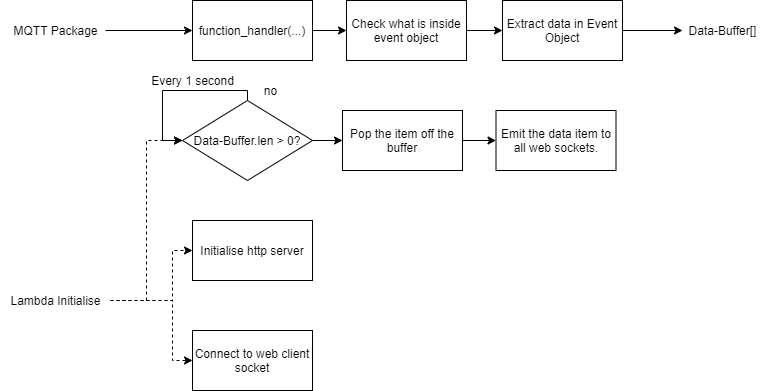
\includegraphics[width=1\linewidth]{pages/Chapter4/Chapter 4 Images/node_web_app.png}
    \caption{Block level diagram explaining systems on the back-end of the Web Server}
    \label{fig:web_app_block_diagram.}
\end{figure}

When the data arrives at the front-end, with the usage of IDs in different HTML tags, it is possible to edit the data within the HTML tag. Since the socket.io emits on a certain keyword. A function is attached to run upon reception of the message with the data from the back-end. The function uses the \textit{document.getElementByID(...)} to edit the text values within the data to the timing values sent by the Lambda functions. The excerpt in Listing \ref{lst:read_socket_data} shows this off.

\begin{lstlisting}[language=HTML, label={lst:read_socket_data}, caption={Reading data sent from the sockets.io connection from the server back-end and editing the front-end HTML page.}]
socket.on('extractTiming', function(extractTiming) {
   let sum = extractTiming.data.DataThroughput + 
        extractTiming.data.PSRetry + extractTiming.data.ChannelStats 
        + extractTiming.data.Assocsta
        + extractTiming.data.PacketetRequested;
        
    document.getElementById('dataTPTime').innerHTML = "DataThroughput.json: <b>" +
        extractTiming.data.DataThroughput.toPrecision(4)+ "s</b>.";
        
    document.getElementById('psRetryTime').innerHTML = "PSRetry.json: <b>" +
        extractTiming.data.PSRetry.toPrecision(4)+ "s</b>.";
        
    document.getElementById('channelStatsTime').innerHTML = "ChannelStats.json: <b>" +
        extractTiming.data.ChannelStats.toPrecision(4)+ "s</b>.";
        
    document.getElementById('assocstaTime').innerHTML = "assocsta.json: <b>" +
        extractTiming.data.Assocsta.toPrecision(4)+ "s</b>.";
        
    document.getElementById('packetReqTime').innerHTML = "PacketRequested.json: <b>" +
        extractTiming.data.PacketetRequested.toPrecision(4)+ "s</b>.";
        
    document.getElementById('extract-time').innerHTML = "Total Extract-Fn Time: <b>"
        + sum.toPrecision(4)+"s</b>";
});
\end{lstlisting}

The code in Listing \ref{lst:read_socket_data} allows for the data shown in Figure \ref{fig:real_time_data_front_end} in bold to be edited in real-time to show the data. First the ID is selected and then the \textit{innerHTML} value is changed to include the type of data and then the timing data is passed via the sockets connection. This listing shows how displayed HTML values can be changed for the Extract Lambda function. The total extract function time, and each data table extraction timing is displayed.

\begin{figure}[ht]
    \centering
    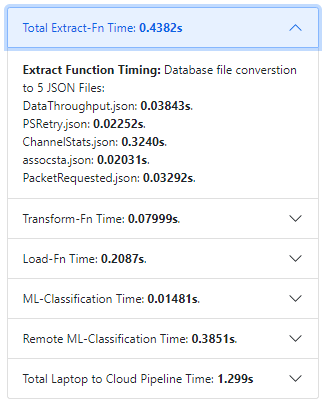
\includegraphics[width=0.5\linewidth]{pages/Chapter4/Chapter 4 Images/newTiming.PNG}
    \caption{Real-time data from Lambda functions to front-end of the Web Application}
    \label{fig:real_time_data_front_end}
\end{figure}

The real-time graph operates in a similar way, where a function is attached to react to messages along a socket.io receive connection. However, rather than editing any given HTML event, the ChartJS \cite{chart_js} package allows a managed real-time graphing application to be embedded onto the website. It also includes appending and removing of data points on the graph in real-time. By using the provided functions this can be done as shown in Listing \ref{lst:append_graph_data_web_app}.

\begin{lstlisting}[language=HTML, caption={How data is updated and removed from the data throughput graph placed centrally in the Web App.}, label={lst:append_graph_data_web_app}]
socket.on('dataTP', function(dataTP) {
    // console.log(dataTP);
    document.getElementById("datatp").innerHTML = dataTP.data;
    time += 0.2;
    addData(myChart,''+time.toPrecision(4)+'s', dataTP.data, 0)
    // console.log("Data queue length is: " + myChart.data.datasets[0].data.length)
    if (myChart.data.datasets[0].data.length > 50) {
        removeData(myChart);
    }
    // $("#datatp").html("currentTP: " + dataTP);
});

\end{lstlisting}

The final implementation of the web application is shown in Figure \ref{fig:impl_web_app}. It follows very closely the design shown in Figure \ref{fig:web_app_design}.

\begin{figure}[ht]
    \centering
    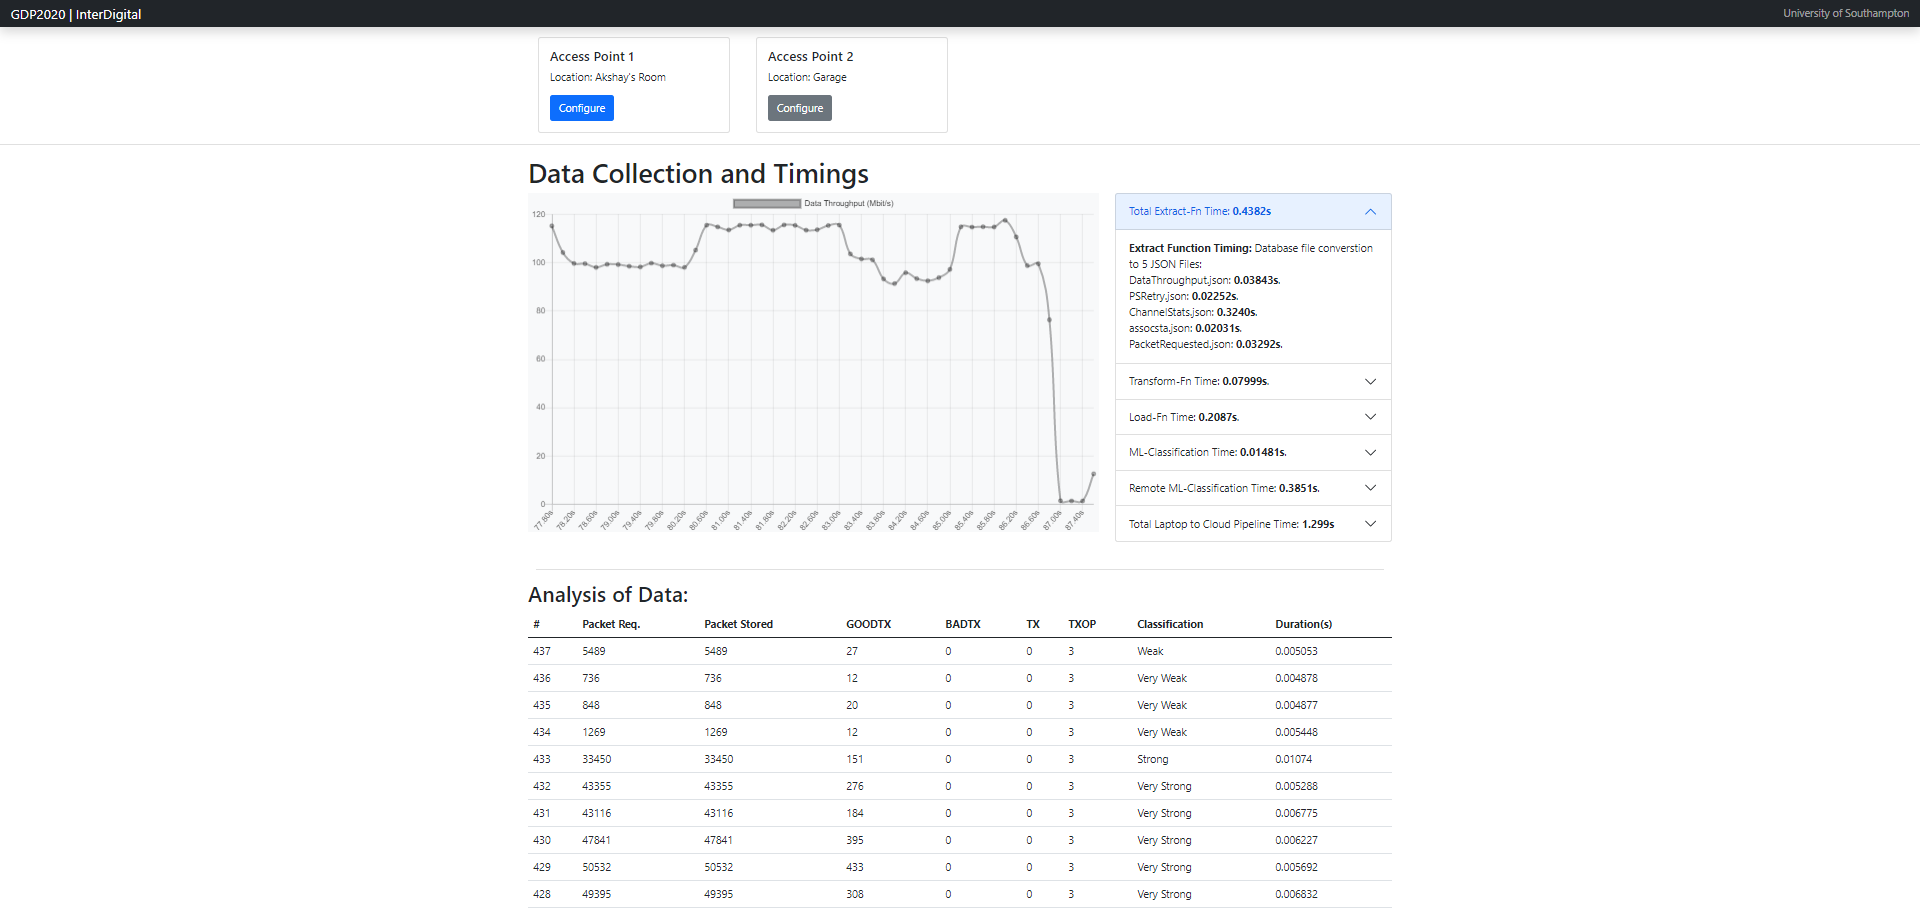
\includegraphics[width=1\linewidth]{pages/Chapter4/Chapter 4 Images/newWebApp.PNG}
    \caption{Fully implemented web application design - The full scale figure can be found in Appendix Section \ref{appendix:full_web_app}}
    \label{fig:impl_web_app}
\end{figure}


\section{Edge Node Technology Exploration - AdvantEDGE} %Syuhada's Section
\subsection{AdvantEDGE Implementation}
The mobile edge emulation platform requires a system that runs on bare Linux operating system (OS) or within virtual machines, and may be installed on a single Kubernetes (K8s) node or a cluster of K8s nodes. The system requirements to install AdvantEDGE include building the runtime environments – Ubuntu, Dockers, Kubernetes, Helm and NVIDIA GPU support. With the system setup, one can clone AdvantEDGE repositories into local host before installing and configure the meepctl tool, a command-line interface (CLI) applications to control the platform. 
Configuring meepctl to the node’s IP address and the directory on the local host, AdvantEDGE binaries can be built to generate the micro-services, as well as the front-end web application. AdvantEDGE micro-services fall into two categories: core and dependencies. Prior to deploying AdvantEDGE core components, dependencies to create micro-services required to run AdvantEDGE can be deployed onto K8s cluster with the meepctl tool and then dockerize these micro-services into container images to be stored into a configured Docker registry. The platform GUI then can be accessed through the standard browser.

To emulate the physical system model, a scenario of the network model can be built by configuring each of the elements needed such as the Internet Cloud, operator, zones, PoA and the edge nodes,  connecting the simulation platform to the physical running native edge application on the server. 

This edge native application is the same Python script used in the AWS IoT Greengrass edge node that is able to extract, transform and load the data before sending them off to the distant cloud. However, prior to connecting the edge application to the AdvantEDGE, the Python application is required to be containerized into Docker image and stored in the Docker registry. Dockerfile, a text document without the extension that contains all the commands a user could call on the command line to assemble an image, has to be created, placed together in the same directory as the Python script and requirement.txt. Requirement.txt is a file that contains the dependencies that the Python script needs to run successfully. This file can be first generated on the command line using \textit{“pip freeze \textgreater\textgreater requirement.txt”}. 

\begin{figure}[ht]
    \centering
    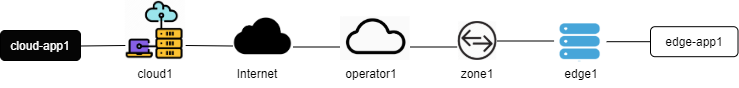
\includegraphics[width=1\linewidth]{pages/Chapter4/Chapter 4 Images/Scenario.png}
    \caption{Scenario created in AdvantEDGE to emulate the physical network topology}
    \label{fig:AdvantEDGE_scenario}
\end{figure}

On AdvantEDGE web GUI, a scenario is created as shown in Figure \ref{fig:AdvantEDGE_scenario}.
The cloud and edge application are connected to the real applications through the configuration where detailed specifications such as group container name, port, protocol, command and arguments need to be provided before deploying the scenario into the sandbox. The scenario then can be deployed once the button on the top right turns green, indicating the server is all good. When executed, one can set the source node and the destination node, to measure the latency, data throughput and traffic metrics in between the nodes after configuring the elements’ network characteristics which can indirectly configure the router. It displays instantaneous measurements for round-trip ping time on the graph if we select to display it on the Network Metrics Point-to-Point.

\begin{lstlisting}[language=Python, caption={Example of Dockerfile}, label={lst:dockerfile}]
# Select the base image to build the new image on top
FROM python:3

# Define the default working directory for any RUN, CMD, ENTRYPOINT, COPY and ADD command
WORKDIR /usr/src/app

# Copy files from Docker host to your Docker image
COPY requirements.txt ./

# Install Python modules required in the requirement.txt
RUN pip install --no-cache-dir -r requirements.txt

# Copy the entire project, recursively into the container for the build
COPY . .

# Execute when the container starts
CMD [ "python", "./python_application.py" ]


# In command line shell to build the image from Dockerfile.
# my-python-app is the name of Docker image that one wants to assign 
$ docker build -t my-python-app .
$ docker run -it --rm --name my-running-app my-python-app

\end{lstlisting}



\section{Cloud Based Processing, Storage and Inference}
The following sections of the report discuss implementations involving Cloud-Based services, i.e. Lambda, Sagemaker, S3, and API Gateway to name a few.
%Anurag's stuff
\subsection{Telemetry Pipeline 1/3 - Triggering Lambda}
One of the three pipelines, involves the transportation of wireless telemetry data directly to the Cloud via the usage of API Gateway and triggering Lambda services. 
\subsubsection{API Gateway Setup to S3 Remote Upload}
The first part to the pipeline to the cloud is the entry into the AWS Cloud. While the possiblity exists to upload directly to S3 via usage of the AWS Command Line Interface (CLI), this is not the preferred way as usage of the Cloud Service cannot be easily monitored and there exists too much control of configurations via the AWS CLI that could be exploited. It is preferred to limit as much access as required to the Cloud from the remote location, primarily for security reasons and for ease of use as well. 

The API Gateway follows the method and resource plan as per the design in Figure \ref{fig:api_gateway_methods}, which described which methods (e.g. POST, GET, PUT, etc...) can be applied to various resources (e.g. .../{s3-bucket}/). To implement the design after setting up the API Gateway, a resource is attached to the address as per Figure \ref{fig:attach_new_resource_api_gateway}. This resource can then be given a name either under \textit{/s3} or further into the s3 address as \textit{/s3/\{bucket\}}.

\begin{figure}[ht]
    \centering
    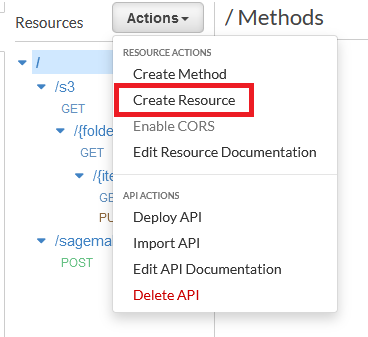
\includegraphics{pages/Chapter4/Chapter 4 Images/create_method_api_gateway.png}
    \caption{Creating a new resource}
    \label{fig:attach_new_resource_api_gateway}
\end{figure}

Once the resource is created and an appropriate name given, then a method can be attached to it. Generally a GET method will be used to retrieve data from the S3 bucket or it can also be used to get a list of all items within the S3 bucket. A PUT method will allow the upload of a unique data object just one time to the S3 Bucket, whereas a POST will allow repeated uploads of the same unique data object. 

The method can be attached to a resource as seen in Figure \ref{fig:attach_new_resource_api_gateway} but instead \textit{Create Method} must be selected. Then from the method execution dashboard in Figure \ref{fig:api_gateway_integration_req}, the integration request options should be selected and a setup similar to the options shown in Figure \ref{fig:integration_request_settings} should be chosen. This will forward the GET request to the S3 endpoint and retrieve the data item or list of items as required.

\begin{figure}[ht]
    \centering
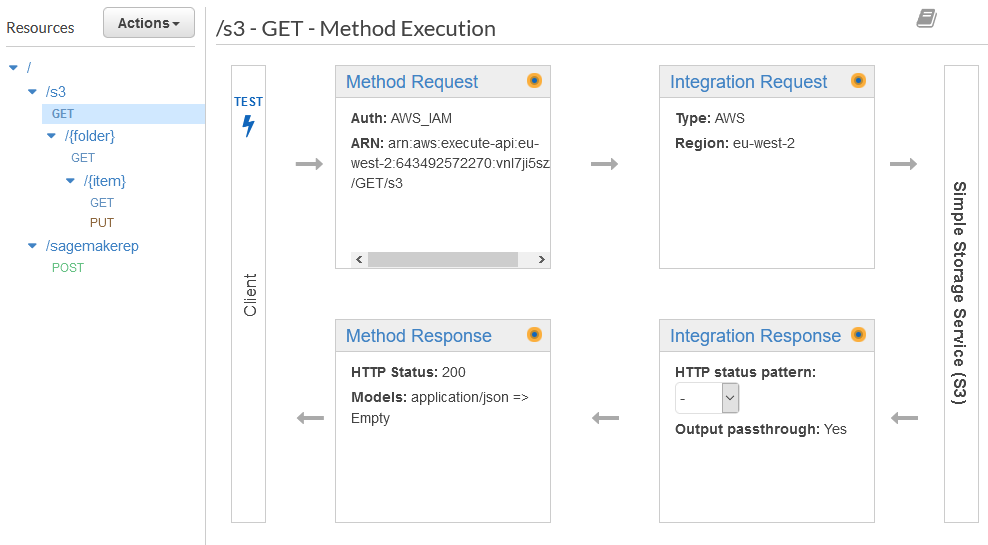
\includegraphics[width=1\linewidth]{pages/Chapter4/Chapter 4 Images/get_method_execution_1.png}
    \caption{Method Execution Dashboard, where settings for security, and redirecting and response settings can be setup}
    \label{fig:api_gateway_integration_req}
\end{figure}

\begin{figure}[ht]
    \centering
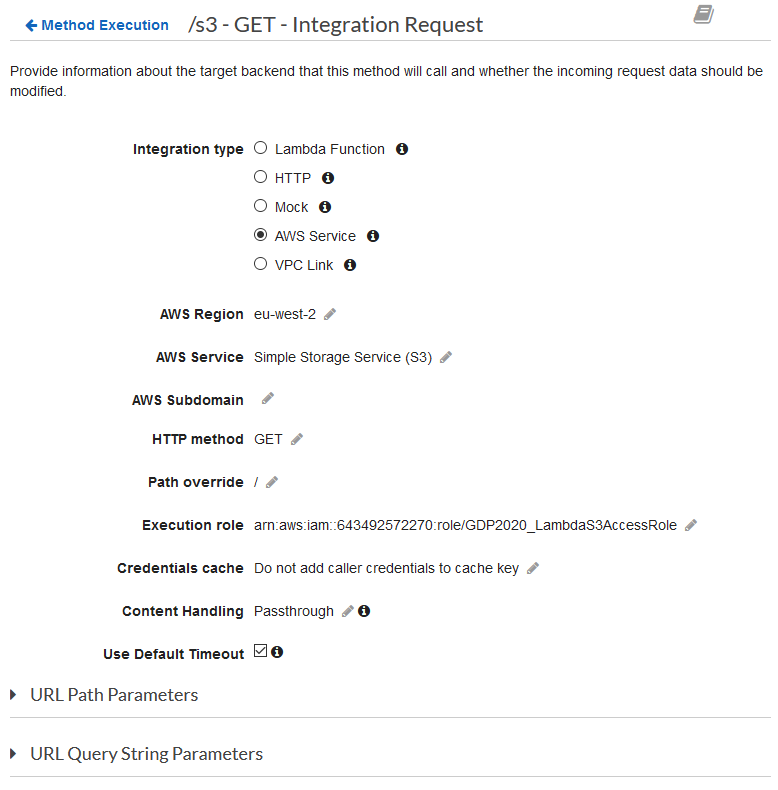
\includegraphics[width=1\linewidth]{pages/Chapter4/Chapter 4 Images/get_method_execution_2.png}
    \caption{Caption}
    \label{fig:integration_request_settings}
\end{figure}

Now the GET request is setup, a similar process must be following to setup the PUT request to the S3 endpoint and now upload to the API Gateway can be completed. To deploy the API Gateway and receive an endpoint URL, the selection in the dropdown menu as seen in Figure \ref{fig:deploy_api_gateway} can be chosen. From this a URL is provided and can be used as the URL to send requests to.

\begin{figure}[ht]
    \centering
    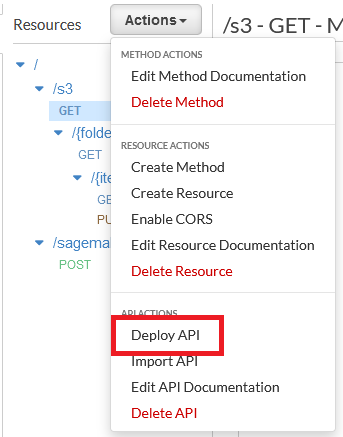
\includegraphics{pages/Chapter4/Chapter 4 Images/deploy_api_gateway.png}
    \caption{How to deploy API Gateway from within the API Gateway dashboard}
    \label{fig:deploy_api_gateway}
\end{figure}


\subsection{Pre-Processing Lambda}
For this section, the implementation of the pre-processing Lambda for the Laptop-To-Cloud pipeline follows a very similar implementation as described in \ref{fig:json_compression}. Where all 5 JSON files extracted from the .db file, must be uploaded into the Lambda function. The main differences being that now the JSON files have been uploaded into an S3 bucket from the laptop, so the cloud-based processing within Lambda is free to handle the processing. 

First the Lambda function must be setup to trigger on S3 create events (which include Put, Post, Update etc...). However, in order to ensure that all 5 JSON files are present before the processing begins, only .complete files are allowed to trigger the Lambda function, as stated in the design section for this pipeline, a .complete file is uploaded only after all 5 JSON files are uploaded.

This triggering on .complete file ensures all files will be available for the compression transformation. The compresson JSON file now sends the data to another S3 bucket (different from the source bucket), so as to avoid cluttering of the S3 bucket. The data can then be used for ML development or for classification as needed.


%Eu Jin's stuff
\subsection{Data Analysis, Pre-processing and Feature Extraction} 

Firstly, telemetry data set consisting of about 800 data points from 3 different devices with different MAC addressed are used in the JSON file format. The bucket containing this data is loaded into the JupyterLab IDE provided by the Sagemaker service.
 
From the telemetry data collected, data for the 5GHz-1 frequency will be investigated and analysed to be used to build the machine learning model. 
The JSON file containing the data is loaded into a data frame as shown in Figure \ref{fig_df}. The columns in the data frame displays the telemetry data parameters of each channel existing in the 2.4GHz, 5GHz-1 and 5GHz-2 bands.

\begin{figure}[ht]
    \centering
    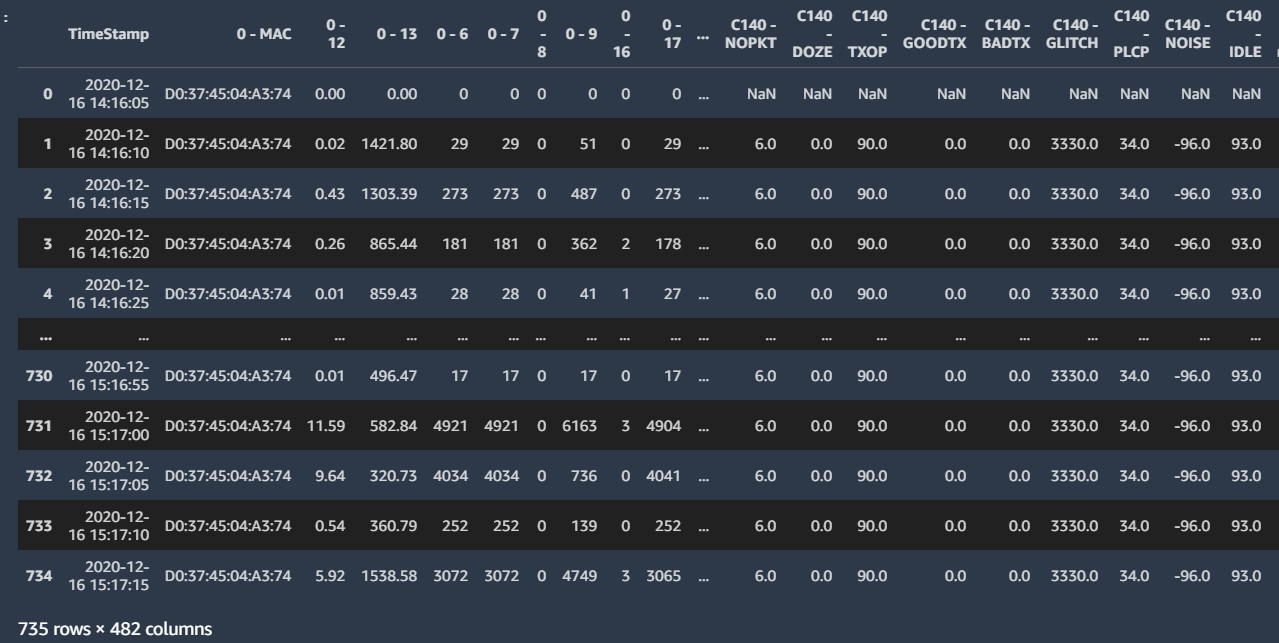
\includegraphics[scale=0.53]{pages/Chapter4/Chapter 4 Images/Dataframe.PNG}
    \caption{Data frame of JSON file.}
    \label{fig_df}
\end{figure}

There exists 8 channels under that particular frequency band which are channels 36, 40, 44, 48, 52, 56, 60 and 64. The parameters for channel 52 were filtered out and used as it is the most active and the other seven channels share the exact same data values. Missing values in the dataset were also removed to ensure uniformity. The data throughput rate for the three devices  respectively were then obtained for analysis shown in Figure \ref{fig_t3} and illustrated using a histogram. From observation of the data throughput rates, the device which is under the process of downloading a game shows the highest variation whereas there is little variation for the other two devices. Thus, the data throughput rate for the first device is filtered out to be used for further analysis. 

\begin{figure}[ht]
    \centering
    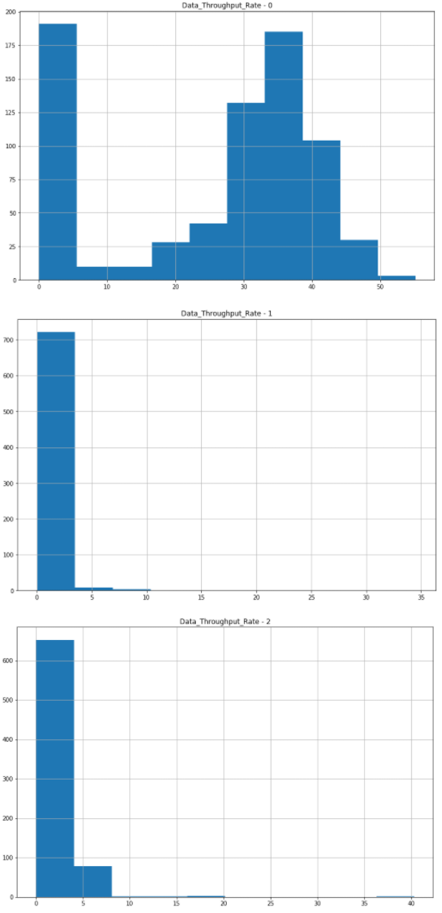
\includegraphics[scale=0.9]{pages/Chapter4/Chapter 4 Images/Throughput.PNG}
    \caption{Data Throughput rate for laptop, mobile phone and respectively}
    \label{fig_t3}
\end{figure}

Next, a heatmap for the correlation matrix which shows the relationship between the parameters of the telemetry data is obtained as shown in Figure \ref{fig_Cmatrix}. 

\begin{figure}[ht]
    \centering
    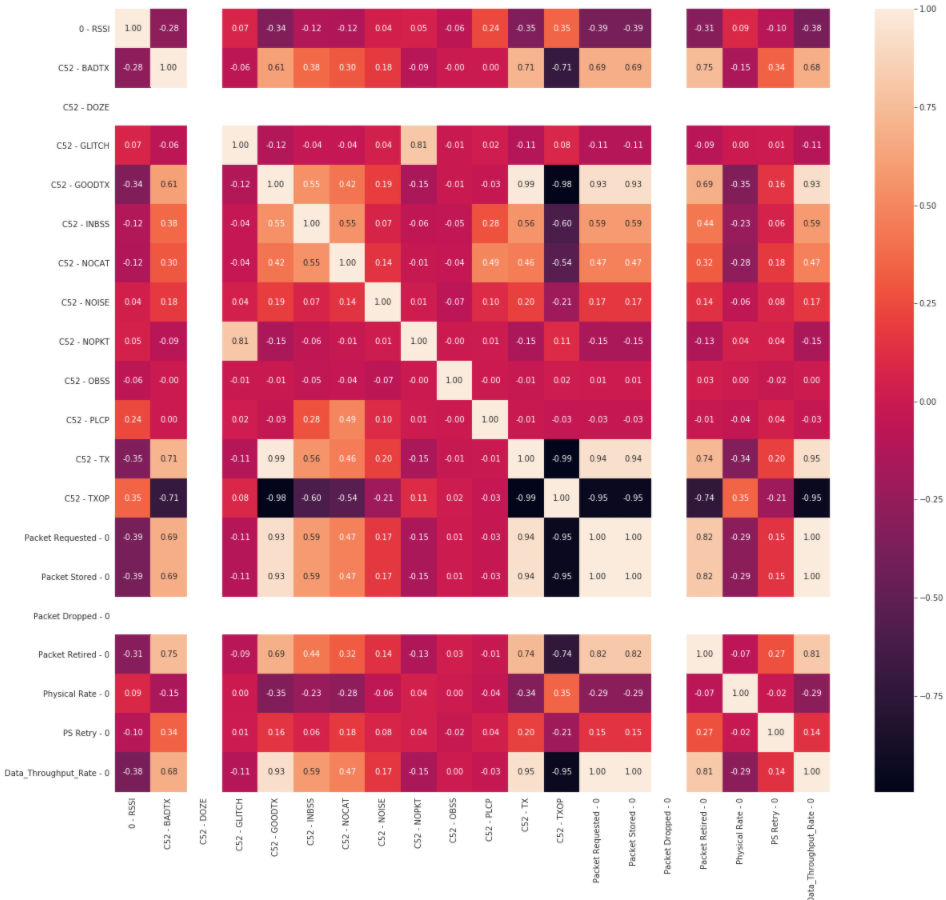
\includegraphics[width=14.5cm,height=15.2cm,keepaspectratio]{pages/Chapter4/Chapter 4 Images/Cmatrix.PNG}
    \caption{Heatmap Correlation Matrix}
    \label{fig_Cmatrix}
\end{figure}

The correlation coefficients were compared between each of the parameters with the data throughput rate. The coefficients were compiled and can be shown in table \ref{table:cc}. 

\begin{table}[ht]
\centering
\begin{center}
\begin{tabular}{ |c|c| } 
  \hline
 Parameters & Correlation coefficient , \textit{r}\\ 
  \hline\hline
 RSSI & -0.38\\ 
 BADTX & 0.68\\ 
 DOZE & -\\ 
 GLITCH & -0.11\\ 
 GOODTX & 0.93\\ 
 INBSS & 0.59\\ 
 NOCAT & 0.47\\ 
 NOISE & 0.17\\\ 
 NOPKT & -0.15\\ 
 OBSS & 0.00\\ 
 PLCP & -0.03\\ 
 TX & 0.95\\ 
 TXOP & -0.95\\ 
 Packet Requested & 1.0\\ 
 Packet Stored & 1.0\\  
 Packet Dropped & -\\ 
 Packet Retired & 0.81\\ 
 Physical Rate & -0.29\\  
 PS Retry & 0.14\\ 
 \hline
\end{tabular}
\caption{Correlation coefficients between the parameters and data throughput rate}
\label{table:cc}
\end{center}
\end{table}

The parameters with coefficient values with intervals of $0.6\leq r \leq 1$ and $-1\leq r \leq -0.6$ are chosen as the features that will be used to train and build the machine learning model. These parameters are chosen as they hold a strong correlation with the data throughput rate which ranges from a moderate to a very strong linear relationship. Therefore, the parameters that will be used as features are as follows: 

\begin{itemize}
    \item GoodTX
    \item BadTX
    \item TX
    \item TXOP
    \item Packet Requested
    \item Packet Stored
    \item Packet Retired
\end{itemize}
 
Bar plots are obtained to show a better illustration of the relationship between the selected parameters on the y-axis and data throughput rate on the x-axis. The relationship between the packet requested, packet stored and packet retired with throughput is shown in Figure \ref{fig_bp1}. From the plot, it can be seen that the three parameters increases with data throughput rate.
Finally, the relationship between the BadTX and TXOP parameters with throughput rate is shown in Figure \ref{fig_bp3}.
\begin{figure} [ht]
    \centering
    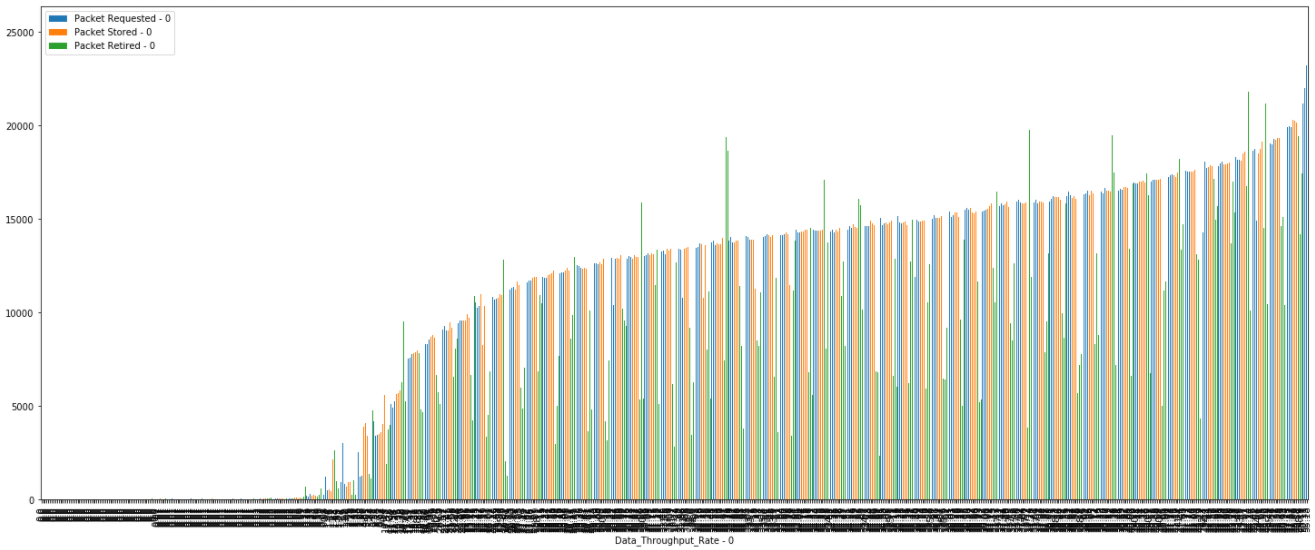
\includegraphics[scale = 0.52]{pages/Chapter4/Chapter 4 Images/Bplot1.PNG}
    \caption{Barplot of Packet Requested, Stored and Retired against Data Throughput Rate}
    \label{fig_bp1}
\end{figure}

Next, the relationship between the TX and GoodTX parameters with throughput rate is shown in Figure \ref{fig_bp2}. When the two parameters increase in value, the data throughput rate also increases.
\begin{figure} [ht]
    \centering
    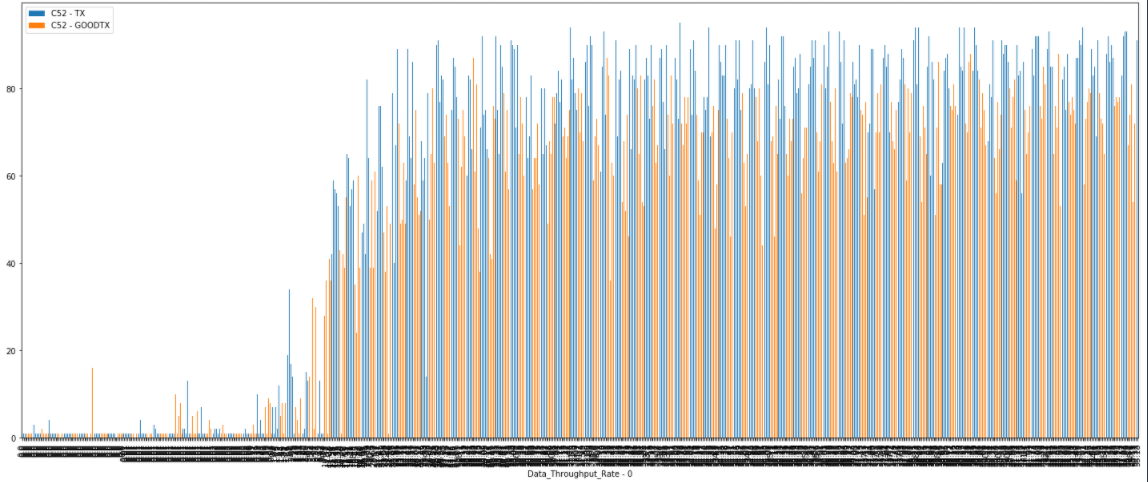
\includegraphics[width=14.6cm,height=200.0cm,keepaspectratio]{pages/Chapter4/Chapter 4 Images/Bplot2.PNG}
    \caption{Barplot of GOODTX and TX against Data Throughput Rate}
    \label{fig_bp2}
\end{figure}

Finally, the relationship between the BadTX and TXOP parameters with throughput rate is shown in Figure \ref{fig_bp3}. From the barplot obtained, the TXOP parameter decreases when the data throughput rate increases. On the other hand, the BadTX increases at a slow rate as the data throughput rate increases.
\begin{figure} [ht]
    \centering
    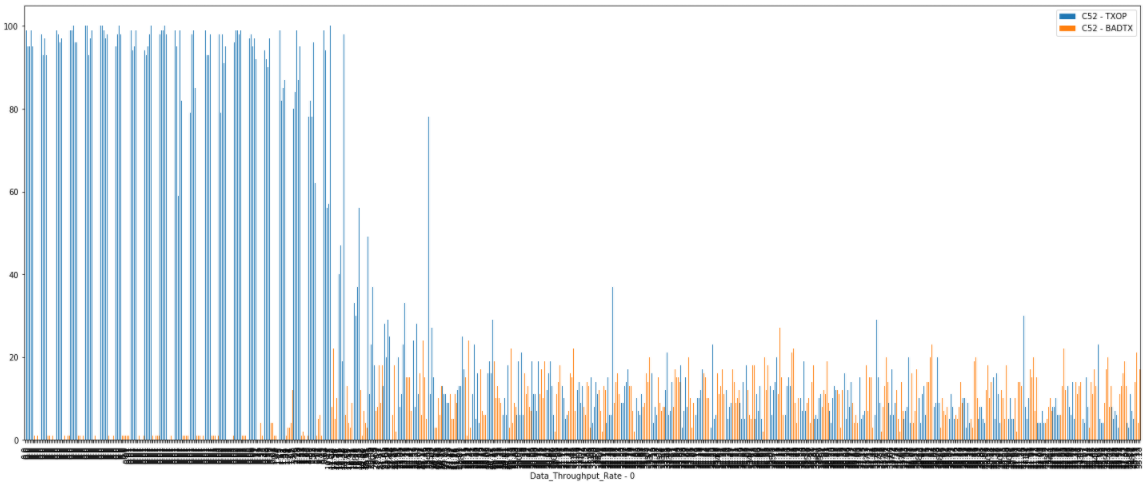
\includegraphics[width=14.6cm,height=200.0cm,keepaspectratio]{pages/Chapter4/Chapter 4 Images/Bplot3.PNG}
    \caption{Barplot of BADTX and TXOP against Data Throughput Rate}
    \label{fig_bp3}
\end{figure}

After this analysis,the creation of the target variable (class) known as data throughput strength based on data throughput rate intervals was implemented and can be shown in table. \ref{table:class}. Five different classes are created: \textbf{Very Weak}, \textbf{Weak}, \textbf{Moderate}, \textbf{Strong} and \textbf{Very Strong}.

\begin{table}[ht]
\centering
\begin{center}
\begin{tabular}{ |c|c| } 
 \hline
 Data Throughput Rate/Mbps & Data Throughput Strength\\ 
  \hline\hline
 0-9 & Very Weak\\ 
 10-19 & Weak\\ 
 20-29 & Moderate \\ 
 30-39 & Strong\\ 
 40 and above & Very Strong\\ 

 \hline
\end{tabular}
\caption{Data Throughput Strength Class implementation based on Data Throughput Rate with 800 Data Points}
\label{table:class}
\end{center}
\end{table}

The seaborn library imported as \textit{sns}, is used to produce a pairplot which shows the distribution between two features in different classes of data throughput strength implemented as shown in Figure \ref{fig_pp}. It also shows the distribution of each feature in the five different classes.

\begin{figure} [ht]
    \centering
    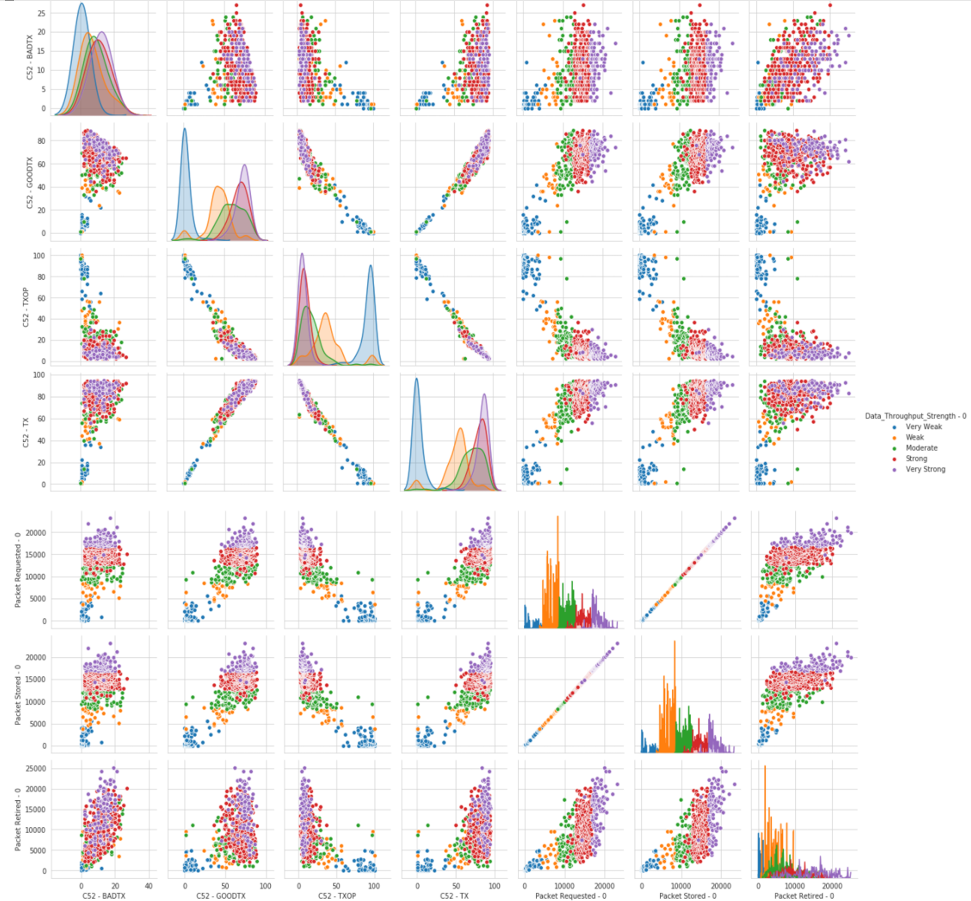
\includegraphics[width=14.6cm,height=200.0cm,keepaspectratio]{pages/Chapter4/Chapter 4 Images/Pairplot.PNG}
    \caption{SNS Pairplot}
    \label{fig_pp}
\end{figure}
 
 From the testing phase in \ref{Section: Testing Phase of ML Model}, the model has an accuracy of 89\% even though it has a high accuracy during the validation phase. This problem occurs because there is too little data and causes overfitting even with the hyperparameters tuned. Thus, a data set containing approximately 6000 data points is collected. The data is preprocessed where the data throughput rate interval for each class were adjusted to accommodate higher rates. The updated interval for each data throughput strength class is shown in Table. \ref{table:class2}.
 
\begin{table}[ht]
\centering
\begin{center}
\begin{tabular}{ |c|c| } 
 \hline
 Data Throughput Rate/Mbps & Data Throughput Strength\\ 
  \hline\hline
0-9 & Very Weak\\ 
10-29 & Weak\\ 
30-49 & Moderate \\ 
50-99 & Strong\\ 
100 and above & Very Strong\\ 

 \hline
\end{tabular}
\caption{Data Throughput Strength Class implementation based on Data Throughput Rate with 6000 Data Points}
\label{table:class2}
\end{center}
\end{table}
 
\subsection{Training and Validation of Machine Learning Model} 
The features are then normalized and prepared to be used to train and build the machine learning model. A clearer workflow of the implementation of training, validating and testing the model is shown in Figure \ref{fig_mlmodel}.

\begin{figure} [ht]
    \centering
    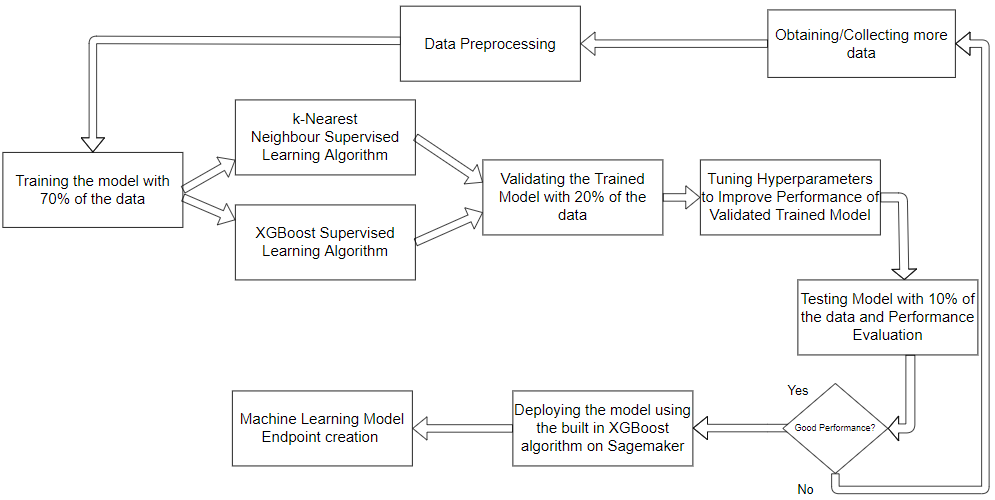
\includegraphics[scale = 0.69]{pages/Chapter4/Chapter 4 Images/Work Flow.PNG}
    \caption{Detailed Block Level Diagram of Machine Learning Model Development}
    \label{fig_mlmodel}
\end{figure}

The dataset is split into a ratio of 70:20:10. 70\% of the data is used to train the model, 20\% of the data is used to validate the model and the remaining 10\% is used to test and evaluate the performance of the final machine learning model. 

\subsubsection{k-Nearest Neighbour Algorithm with Scikit-Learn}
The k-Nearest Neighbour supervised learning algorithm is used to build the model within Sagemaker without deployment. The model is validated with the validation set after it is being trained. Several hyperparameters are tuned such as the number of neighbours, \textit{k} and the distance function to improve the performance of the trained model. The value of k is varied from 1 to 10 with two different distance functions which are the Euclidean and Manhattan functions. The performance of the trained model using the validation set is measured with the accuracy metric. The results are transferred into a table shown in Table \ref{table:euclidean} and Table \ref{table:manhattan} respectively.

\begin{table}[ht]
\centering
\begin{center}
\begin{tabular}{ |c|c| } 
  \hline
 The number of neighbors, k  & Accuracy/\%\\ 
  \hline\hline
1 & 95.9\\ 
2 & 96.6\\ 
3 & 95.9\\ 
4 & 98.6\\ 
5 & 96.6\\ 
6 & 95.9\\ 
7 & 97.3\\ 
8 & 96.6\\\ 
9 & 97.3\\ 
10 & 95.9\\ 
\hline
\end{tabular}
\caption{Accuracy of validated trained model using the Euclidean distance function }
\label{table:euclidean}
\end{center}
\end{table}

\begin{table}[ht]
\centering
\begin{center}
\begin{tabular}{ |c|c| } 
  \hline
 The number of neighbors, k  & Accuracy/\%\\ 
  \hline\hline
1 & 95.2\\ 
2 & 98.6\\ 
3 & 97.3\\ 
4 & 98.6\\ 
5 & 97.3\\ 
6 & 97.3\\ 
7 & 97.9\\ 
8 & 97.9\\\ 
9 & 97.3\\ 
10 & 96.6\\ 

 \hline
\end{tabular}
\caption{Accuracy of validated trained model using the Manhattan distance function}
\label{table:manhattan}
\end{center}
\end{table}
 
From the validation results with the Euclidean distance function , the \textit{k} value of 4 gives the best performance with an accuracy of 98.6\%. For the results with the Manhattan distance function, a \textit{k} value of also gives the same accuracy of about 98.6\%. Therefore, both distance functions with a \textit{k} value of 4 can be used to train the model and evaluate the model performance with the test data.


Next, the model is retrained with the k-Nearest Neighbour algorithm using the 6000 data points collected. The hyperparameters were maintained and used in the training and validating phases. The results of the trained model with the validation set is recorded in Table \ref{table:euclidean2} and Table \ref{table:manhattan2} respectively.
\begin{table}[ht]
\centering
\begin{center}
\begin{tabular}{ |c|c| } 
  \hline
 The number of neighbors, k  & Accuracy/\%\\ 
  \hline\hline
1 & 97.8\\ 
2 & 97.4\\ 
3 & 98.2\\ 
4 & 98.2\\ 
5 & 98.3\\ 
6 & 98.4\\ 
7 & 98.6\\ 
8 & 98.5\\ 
9 & 98.6\\ 
10 & 98.3\\ 
\hline
\end{tabular}
\caption{Accuracy of validated trained model using the Euclidean distance function }
\label{table:euclidean2}
\end{center}
\end{table}

\begin{table}[ht]
\centering
\begin{center}
\begin{tabular}{ |c|c| } 
  \hline
 The number of neighbors, k  & Accuracy/\%\\ 
  \hline\hline
1 & 97.8\\ 
2 & 97.5\\ 
3 & 98.2\\ 
4 & 98.1\\ 
5 & 98.3\\ 
6 & 98.3\\ 
7 & 98.6\\ 
8 & 98.5\\\ 
9 & 98.4\\ 
10 & 98.3\\ 

 \hline
\end{tabular}
\caption{Accuracy of validated trained model using the Manhattan distance function}
\label{table:manhattan2}
\end{center}
\end{table}

\subsubsection{XGBoost Algorithm with Sagemaker Python SDK}
\label{xgboost-training}
Next, the built-in XGBoost supervised learning algorithm within Sagemaker is used to train and deploy the model. There are several steps required to prepare the data before training the model with the Sagemaker Python SDK. Firstly, the class of each data point has to be encoded with numeric values. The numeric values which represents each class is shown in Table \ref{table:class}. 
The column containing the class (target variable) has to be moved to the first column in the dataframe with its name removed. The dataset is then converted and stored as a CSV file. The XGBoost algorithm version 1.2-1 is used for the model training. The hyperparameters used are shown in table \ref{table:xg}. The training process can be shown in Figure \ref{fig_train}.

\begin{figure} [ht]
    \centering
    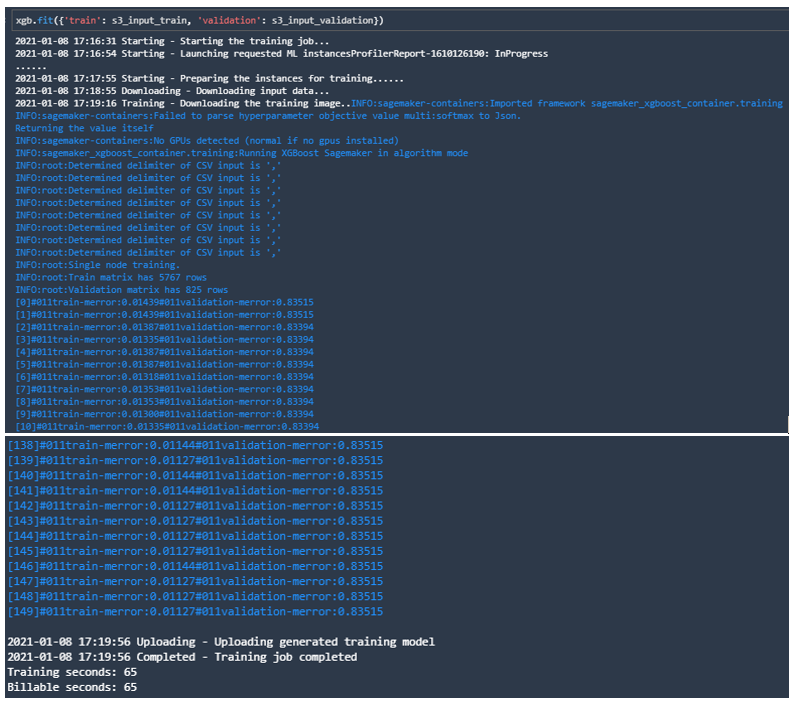
\includegraphics[scale = 0.8]{pages/Chapter4/Chapter 4 Images/Training.PNG}
    \caption{Snippet of Training the Machine Learning Model in Sagemaker}
    \label{fig_train}
\end{figure}

After the model is trained with this algorithm, it will then be deployed with an endpoint being created. A variable will be created for the deployed trained model. This variable can then be used to validate the trained model using the validation data set. The accuracy of obtained for the validated trained model is about 28.4\% for the dataset containing approximately 800 data points. The hyperparameters were adjusted and still returns a low accuracy classifier.
On the other hand, the accuracy obtained for the validated trained model is about 98.8\% for the dataset containing approximately 6000 data points.

\begin{table}[ht]
\centering
\begin{center}
\begin{tabular}{ |c|c| } 
  \hline
 Class  & Numeric Value\\ 
  \hline\hline
Moderate & 0\\ 
Strong & 1\\ 
Very Strong & 2\\ 
Very Weak & 3\\ 
Weak & 4\\ 

 \hline
\end{tabular}
\caption{Numeric Representation for Each Class}
\label{table:class}
\end{center}
\end{table}

\begin{table}[ht]
\centering
\begin{center}
\begin{tabular}{ |c|c| } 
  \hline
Hyperparameters  & Values\\ 
  \hline\hline
Max depth & 4\\ 
Learning rate (eta) & 0.2\\ 
Gamma & 4\\ 
Subsample & 0.5\\ 
Number of rounds & 150\\ 


 \hline
\end{tabular}
\caption{Hyperparameters for XGBoost Model}
\label{table:xg}
\end{center}
\end{table}

\subsection{Deploying Sagemaker Endpoint} 
When the machine learning model is deployed, an endpoint will be created during the process which can be shown in Figure \ref{fig_endpoint}. For example, the endpoint created for the deployed model has a name called ``sagemaker-xgboost-2020-12-22-20-52-53-943''. 

\begin{figure} [ht]
    \centering
    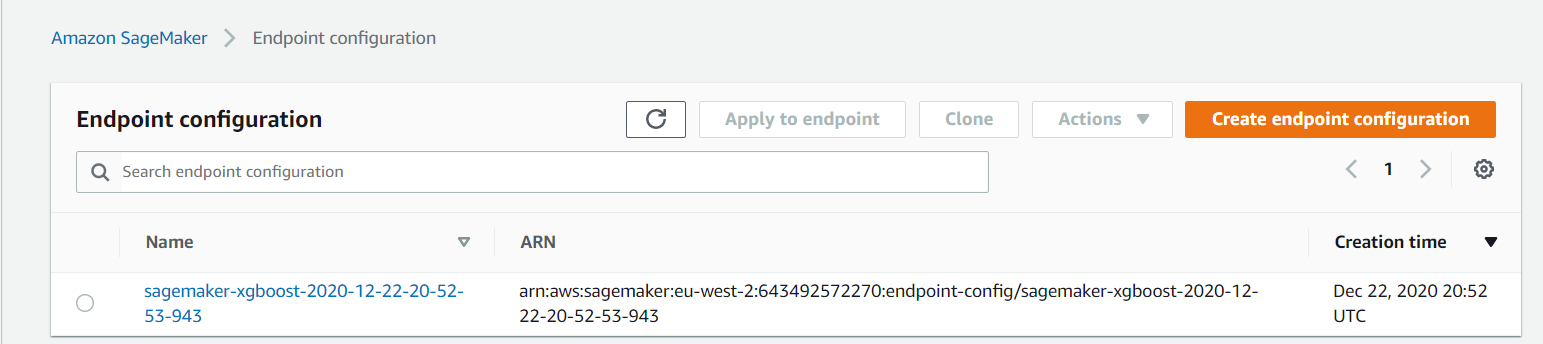
\includegraphics[scale= 0.44]{pages/Chapter4/Chapter 4 Images/Endpoint.PNG}
    \caption{Endpoint Creation}
    \label{fig_endpoint}
\end{figure}

This endpoint of the trained model can be invoked using Amazon API Gateway and AWS Lambda where it can be used to predict or classify data. A Lambda function is first created to call the Sagemaker runtime invoke endpoint. During this stage, the policy of the IAM execution role is edited such that it gives permission to the Lambda function to invoke the model endpoint which can be shown in Figure \ref{fig_policy}. 

\begin{figure} [ht]
    \centering
    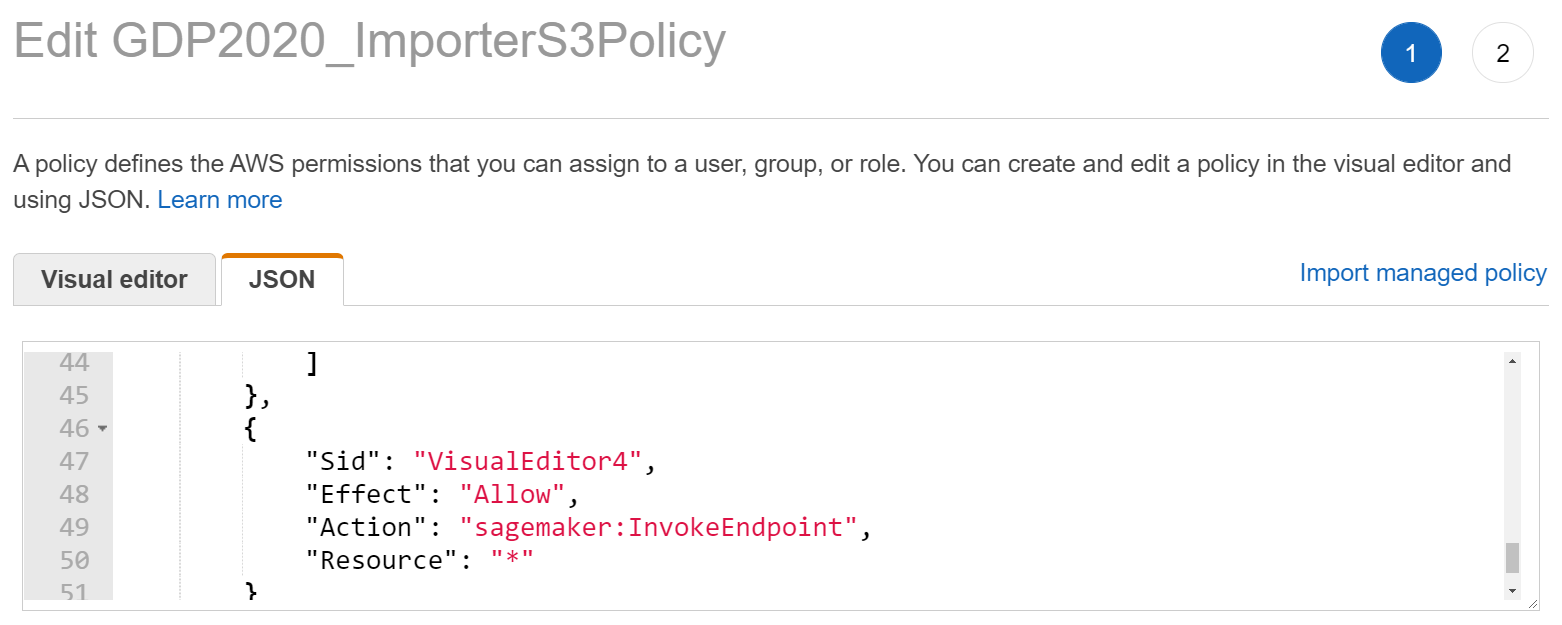
\includegraphics[scale =0.43]{pages/Chapter4/Chapter 4 Images/Policy.PNG}
    \caption{Policy Added for Endpoint Permission Access by the Lambda Function}
    \label{fig_policy}
\end{figure}

Next, the endpoint name is included in the environment variable for the Lambda function which will be made available to the code for the invocation request. This step can be shown in Figure \ref{fig_env}. 

\begin{figure} [ht]
    \centering
    \includegraphics[width=14.0cm,height=2.5cm,scale =0.45]{pages/Chapter4/Chapter 4 Images/ENVIRON.PNG}
    \caption{Environmental Variable}
    \label{fig_env}
\end{figure}

Moving on forward, an API Gateway is created where it triggers an event that invokes the Lambda function. The event triggered would be the test data passing through it. The final setup of the API Gateway is shown in Figure \ref{fig_api}. An invoke URL will be obtained when the API Gateway is deployed. 

\begin{figure} [ht]
    \centering
    \includegraphics[width=14.6cm,height=200.0cm,keepaspectratio]{pages/Chapter4/Chapter 4 Images/API Gateway.PNG}
    \caption{API Gateway setup for Lambda function to Invoke Endpoint}
    \label{fig_api}
\end{figure}


  
% \section{Machine Learning Model Deployment}
\section{Over-the-top Application using ML Model Outputs and Input Data}
\subsection{Web Application}

%% ----------------------------------------------------
\chapter{Testing} \label{Chapter: Testing}


% PR Anurag -Complete 1


\section{Data Retrieval} \label{Section: Testing Data Retrieval}

In Section \ref{Section: Data collection from the Router}, three different methods of data retrieval were implemented (Tampermonkey, Selenium WebDriver and SSH). All three methods principally worked the same, in that they periodically downloaded the database file every 5 seconds, but there are some core differences that set them apart. For instance Tampermonkey required the user to manually login to the ASUS Router and navigate to the data collection configuration page. From there the userscript would start the data collection process and download the database files. Due to the fact that Tampermonkey is a Google Chrome extension, the Chrome window must be kept open and the userscript is not compatible with other internet browsers (but there are similar extensions for other browsers). Additionally, running the data retrieval process on Google Chrome is resource intensive because of the inherent resource hog nature of its design. Using Selenium WebDriver, the login and navigation to the configuration page is automatically completed by the program. From there the Python script will start the data collection and download the database files. Selenium WebDriver uses ChromeDriver as the main interface for the data retrieval process, and once again this application must be kept open for the duration of the data collection process and due to its use of Chrome it is also resource intensive. The SSH method will connect and login to the ASUS router and periodically download the database file. All that is required of the user is to start the data collection process on the ASUS Web GUI, and from there the program will run in the background without the use of any other applications. 

With all three methods thoroughly tested and considered, the SSH method was chosen as the way to retrieve the from the ASUS router. The main reasons for this is the fact that this method is not dependent on any certain applications, it allows for the retrieval process to fully run in the background and is also the least resource intensive method.

\section{Data Collection For Testing}

In order to test the functionality of the Machine Learning model, data collection under specific environment conditions had to be conducted. Since data throughput is used as the main parameter for the ML classification, this parameter is also the main focus of the environment test. Initially datasets for training and testing were recorded while doing particular tasks such as downloading large files, watching high resolution videos and general web browsing in order to diversify the values of data throughput. However, this proved to be a very inefficient as it is difficult to control the actual values of data throughput recorded by the router. 

\subsection{StarTrinity Software: CST}

StarTrinity CST is a continuous internet speed test tool, which allows for long stress test duration with the download and upload bandwidth to be fixed \cite{CST}. This tool was used to generate test datasets with specific data throughput values, which fit within the ML classifications shown in Table \ref{table:class}. This tool is also used in the live testing and demonstration of the whole system in order to show the accuracy of the ML model across the entire range of data throughput values. 

\begin{figure} [ht]
    \centering
    \includegraphics[width=1\linewidth]{pages/Chapter5/Chapter 5 images/CST.PNG}
    \caption{StarTrinity Software: Continuous Speed Test}
    \label{fig_CST}
\end{figure}

\section{Data Upload and Storage}

As mentioned in Chapter \ref{Chapter:System Design}, one of the telemetry pipelines is the direct upload of the data from the Laptop to the Cloud. This testing was conducted using the Selenium WebDriver to retrieve the data periodically, the script then detects a new database file and triggers the JSON conversion (Section \ref{section:Data Extraction}). Once this conversion is completed the files are uploaded to the Cloud (Section \ref{Section:pipeline1/3}). 

Figure \ref{fig_uploadData} shows the conversion functions operating, with their timings, and then the complete messages for the direct upload of data to the S3 Bucket with their respective timestamps. Figure \ref{fig_s3Upload} \& \ref{fig_s3UploadFolder} shows the data has been successfully uploaded along with .complete file. 

\begin{figure} [ht]
    \centering
    \includegraphics[width=1\linewidth]{pages/Chapter5/Chapter 5 images/dataUpload.PNG}
    \caption{Data Upload From Laptop Direct to S3 Bucket}
    \label{fig_uploadData}
\end{figure}

\begin{figure} [ht]
    \centering
    \includegraphics[width=1\linewidth]{pages/Chapter5/Chapter 5 images/s3Upload.PNG}
    \caption{S3 Bucket Proof of Upload with Data Folder and .complete File}
    \label{fig_s3Upload}
\end{figure}

\begin{figure} [ht]
    \centering
    \includegraphics[width=1\linewidth]{pages/Chapter5/Chapter 5 images/s3UploadFolder.PNG}
    \caption{S3 Bucket Proof of Upload of Individual JSON Files}
    \label{fig_s3UploadFolder}
\end{figure}
% PR Eu Jin -COMPLETE 1
\section{AWS IoT Greengrass / Edge Node Deployment}
\subsection{Extract, Transform and Load Testing}
The testing of the localised Lambda funcitons were completed individually one function at a time. As each Lambda function sends MQQT messages to the IoT Cloud via various subscriptions and topics, these were monitored to see correct functionality of the function. These topics and subscriptions were all discussed in the previous sections and are seen more specifically within Figure \ref{fig:mqqt_testing_setup}
\subsubsection{Extract Lambda Function}
There are three topics that the extract function outputs onto:
\begin{itemize}
    \item extract/checkFile
    \item extract/json
    \item transform/ready
\end{itemize}
The, first item is the \textit{extract/checkFile} which is constantly looking for a .db file placed into the shared directory between the Edge Node and the connected User-Endpoint to the wireless access point.  These output messages can be seen in Figure \ref{fig:extract_checkFile}. Initially no .db file is seen. Upon a .db file being placed into the shared directory, the extract function opens the file and then confirms it is able to open it.

\begin{figure}[ht]
    \centering
    \includegraphics[width=1\linewidth]{pages/Chapter5/Chapter 5 images/Lambda-Fns/extract_checkFile.png}
    \caption{Output of MQQT Packets sent to IoT Cloud from the Extract Lambda Function}
    \label{fig:extract_checkFile}
\end{figure}

The second item is the \textit{extract/json}, which is the timing taken for each data table to be extracted from the .db file. As these are completed, they are assembled into a JSON object and published to the topic. The output of this is similar to the messages sent to the Web Application as the timing data is contained within as seen in Figure \ref{fig:extract_json}.

\begin{figure}[ht]
    \centering
    \includegraphics[width=1\linewidth]{pages/Chapter5/Chapter 5 images/Lambda-Fns/extract_json.png}
    \caption{Output of Extraction of JSON Files from Data-table from the .db File}
    \label{fig:extract_json}
\end{figure}

The extract-function then sends the current time that the output file was generated, this time also happens to be pre-pended onto the output JSON files, hence is needed by the transform function to open the newly generated files correctly. This message from one Lambda function to another is seen in Figure \ref{fig:transform_ready}.

\begin{figure}[ht]
    \centering
    \includegraphics[width=0.7\linewidth]{pages/Chapter5/Chapter 5 images/Lambda-Fns/transform_ready.png}
    \caption{Telling the Transform function to wake and the name of the files to be opened.}
    \label{fig:transform_ready}
\end{figure}

\subsubsection{Transform Lambda Function}
The transform function sends out two MQQT packages under the topics of:
\begin{itemize}
    \item transform/load
    \item transform/extract
\end{itemize}

Once the data within \textit{transform/ready} is sent, and more specifically the \textit{TimeStamp} data, which contains a string that the new 5 generated files begin with, the transform function can begin its correct operation. As it can be seen in Figure \ref{fig:transform_load}, each of the 5 JSON file names begin with the name given in the \textit{gTimeStamp} value. This would not be possible as the timestamp changes from every new db file inserted into the shared folder. After each JSON file is uploaded, a \textit{Succesfully Load JSON files} message is provided to indicate files were all succesfully found. These load messages are sent along the \textit{transform/load} topic.

\begin{figure}[ht]
    \centering
    \includegraphics[width=0.7\linewidth]{pages/Chapter5/Chapter 5 images/Lambda-Fns/transform_load.png}
    \caption{Transform function loads the 5 JSON files}
    \label{fig:transform_load}
\end{figure}

Upon loading of the files, data must then be extracted and compressed to a single JSON file. A short and curt message here is enough to indicate the process has been completed and the new JSON file has been stored into all three new locations, for the Load, Local-ML and Remote-ML functions, and is sent across the \textit{transform/extract} topic.

\begin{figure}[ht]
    \centering
    \includegraphics[width=0.5\linewidth]{pages/Chapter5/Chapter 5 images/Lambda-Fns/transform_extract.png}
    \caption{Tranform Function has completed its compression and saving tasks for these 5 new JSON files}
    \label{fig:my_label}
\end{figure}

\subsubsection{Load Lambda Function}
From this Lambda function, the compressed JSON file is uploaded to S3 for storage and any long term analysis. The main topics for testing purposes that this Lambda function is subscribed to are as follows:
\begin{itemize}
    \item load/checkFile
    \item load/uploadFile
\end{itemize}

This Lambda function has a basic task, but first must load the JSON file into the program. This is done by continually checking the directory for \textit{/dest/Stream-Upload/...}. If anything is found here, it will load the JSON files found one at a time. The first topic that is published to by the Lambda function, \textit{load/checkFile}, outputs every 5 seconds to what files it can see in the directory it searches in for JSON files. Upon finding a JSON file, it loads that specific JSON file and this is seen in Figure \ref{fig:load_checkFile}. The lowest message shows an empty directory, then after 5 seconds it is checked again and a new JSON file is found and is then loaded and shown to be loaded succesfully.



\begin{figure}[ht]
    \centering
    \includegraphics[width=1\linewidth]{pages/Chapter5/Chapter 5 images/Lambda-Fns/load_checkFile.png}
    \caption{MQQT Packets seen after loading JSON file}
    \label{fig:load_checkFile}
\end{figure}

Once the JSON file is loaded and the JSON data is extracted, then a request payload is formed, with the body of the payload as the JSON object as discussed in the designed section and the headers as required for correct authentication to the endpoint. Upon receiving a status code of the 200 after sending the put request, the lambda function will then publish onto the topic, \textit{load/uploadFile} that the function succesfully completed as seen in Figure \ref{fig:load_uploadFile}. 

\begin{figure}[ht]
    \centering
    \includegraphics[width=1\linewidth]{pages/Chapter5/Chapter 5 images/Lambda-Fns/load_fileUpload.png}
    \caption{Upon successful upload to S3, this message is sent to the IoT Cloud}
    \label{fig:load_uploadFile}
\end{figure}


\subsubsection{Local-ML Inference Testing}
For the Local-ML Inference testing, the testing method is shown in a different format. The IoT Cloud Method is already shown off, however another method is for the output data and timings to be written to a file. In this output file, data that has been already filtered to fit the model's required input format, timing data and classification by the model is written into the file. Since this model classification and data output must also be verified by other members of the project, it is important to also have this output data stored. An example of one timestamp's set of input data for the model is shown in Figure \ref{fig:local-ml-output}, where the data input set of \textbf{[0,0,0,0,0,1,95]} correctly corresponds to '3.0' or 'Very Weak'. This data output is stored and then transferred for model verification and it also transferred as MQQT Packages to the Web Server for live data viewing. This latter point is discussed further in the Web Application testing.

\begin{figure}[ht]
    \centering
    \includegraphics[width=0.5\linewidth]{pages/Chapter5/Chapter 5 images/Lambda-Fns/local_ml_fn_output.png}
    \caption{Local Machine Learning Lambda Function's Output Format}
    \label{fig:local-ml-output}
\end{figure}

The output here shows correct operation as is discussed in the ML Sections of the project and how the value of this classification corresponds to the equivalent of 'Very Weak' data throughput.


\subsubsection{Remote-ML Inference Testing}
The Remote-ML Inference testing simply uses an API Endpoint which is tested using Post Man in Section \ref{post_man_testing}. The Lambda function uses the Python requests library to package and sends the JSON data to the Cloud for classification. The response is shown in the mentioned section further in the report. The data received by the post request is then transferred to the Web App directly for live viewing.


\subsection{NodeJS Web Server Application}
The web application is being used for live-data viewing to see data being handled in the back-end and how long it took each Lambda function for processing in the various stages and transfer to the Cloud. For the testing of the NodeJS Web Server Application, all systems were needed to be running. These includes the automatic data retrieval from the SSH; transfer of files from the laptop to the edge node; ETL on the incoming data and then provisioning the ML Model for localised inference of the data throughput based on Channel Stats; ML-inference is also seen by sending the input data parameters to the cloud and getting inference directly from the Sagemaker endpoint. 

\begin{figure}[ht]
    \centering
    \includegraphics[width=1\linewidth]{pages/Chapter5/Chapter 5 images/testing_node_js_manually.png}
    \caption{Feeding the Edge Node directory }
    \label{fig:feeding_edge_node_manually}
\end{figure}
The first test however, would be to manually feed the edge-node with .db files and seeing the response of the developed Web Application. This method is shown in Figure \ref{fig:feeding_edge_node_manually}. The twelve files are inserted into the shared directory one at a time. As soon as the Edge Node begins processing, data can be seen streaming into the Web Server. In the first image shown in Figure \ref{fig:node_testing_1}, the data can be seen as having been processed by the extract and transform functions. The Load function has not been completed but the ML-Local inference has begun processing. The data throughput and classification data appearing in the table proves this, and as the Local-ML total timing has not yet been shown it can be deduced that the Local-ML is still running. The completed duration to scan and run each file within the Lambda functions is shown on the right. The remote, cloud-based ML Model is unreachable and goes to prove why deploying models to local environments is so useful in this testing example.
\begin{figure}[ht]
    \centering
    \includegraphics[width=1\linewidth]{pages/Chapter5/Chapter 5 images/testing_pt1.png}
    \caption{Data has been processed by Extract and Transform Lambda functions, and is still being processed by Load and Local-ML Lambda functions}
    \label{fig:node_testing_1}
\end{figure}

The final live-data view for one .db file is seen in Figure \ref{fig:node_testing_2}.A few key timings can be seen:
\begin{itemize}
    \item Extraction from .db File: \textbf{0.15s}
    \item Transformation time to compress into a single JSON file: \textbf{0.44s}
    \item Load time of compressed JSON to S3: \textbf{1.743s}
    \item Local-ML classificaiton of the whole file: \textbf{0.58s}
    \item Remote-ML Classification time: \textbf{n/a}
\end{itemize}
A full comparison between Local-ML and Remote-ML will be shown in the Results section, but correct operation of the NodeJS Web application was shown and therefore can be used for testing and validation of the deployed model.
\begin{figure}[ht]
    \centering
    \includegraphics[width=1\linewidth]{pages/Chapter5/Chapter 5 images/testing_pt2.png}
    \caption{Full testing with Manual .db File Placement.}
    \label{fig:node_testing_2}
\end{figure}

% PR Syuhada
\section{Testing Phase of Machine Learning Model with Test Dataset} \label{Section: Testing Phase of ML Model}
\subsection{Data Throughput Strength Classifier}
The trained machine learning model (classifier) is evaluated with the test set which contains 10\% of the data set. The performance of the data throughput strength classifier is illustrated in a confusion matrix by making use of the heatmap function available. The vertical columns represent the predicted class while the horizontal rows represent the actual class of the data points. A classification report is also produced to evaluate the performance of the classifier which displays measurement metrics such as accuracy, recall, precision, and F1-score. 

\subsubsection{k-NN Algorithm with 800 Data Points}
Firstly, the model built with the k-Nearest Neighbour algorithm using the 800 data points is first tested. The confusion matrix for the model is shown in Fig. \ref{fig_cm1}.The diagonal values in the matrix represent the correctly classified data points with respect to their classes. Data points outside of the diagonal values are misclassified points. For example, there are four points from the `Strong' data throughput class misclassified under the `Moderate' data throughput class. One data point from the `Moderate' class was misclassified as the `Weak' class. Next, three data points from the `Very Strong' class were misclassified as the 'Strong' class.

\begin{figure} [ht]
    \centering
    \includegraphics[scale=1.0]{pages/Chapter5/Chapter 5 images/knn_800.PNG}
    \caption{Confusion matrix of Data Throughput Strength Classifier}
    \label{fig_cm1}
\end{figure}

A classification report for the tested model is shown in Figure \ref{fig_crknn}. The precision, recall and F1-score for each class is also displayed. The support column shows the actual amount of data points that belong to their corresponding classes. The `macro avg' represents the average precision, recall and F1-score across the five classes. The `weighted avg' shows the average of the three metrics where the metric of each class is multiplied by a weight during the calculation of the average values. This step is done to give a better average value when there are imbalance data points across the five classes of data.  

The accuracy achieved by the model is 89.2\%. The weighted average values of precision, recall and F1-score obtained are 90.5\%, 89.2\% and 89.2\% which is fairly good.  

\begin{figure} [ht]
    \centering
    \includegraphics[scale=1.3]{pages/Chapter5/Chapter 5 images/C_report_knn.PNG}
    \caption{Classification report of the k-NN classifier}
    \label{fig_crknn}
\end{figure}


\subsubsection{k-NN Algorithm with 6000 Data Points}
The confusion matrix is produced for the trained model with the 6000 data points and can be shown in  Fig. \ref{fig_cm1}. Five data points from the `Very Strong' class were misclassified as the `Strong' class while three data points from the `Weak' class were misclassified as the `Very Weak' class. One point from the `Moderate' class were misclassified as the `Weak' class.

\begin{figure} [ht]
    \centering
    \includegraphics[scale=1.0]{pages/Chapter5/Chapter 5 images/knn_6k.PNG}
    \caption{Confusion matrix of Data Throughput Strength Classifier}
    \label{fig_cm1}
\end{figure}

The classification report for the tested model is obtained. The accuracy achieved by the model is approximately 98.6\%. The weighted average precision, recall and F1-score obtained are 98.7\%, 98.6\% and 98.6\% respectively. This model has a better performance than the previous model. Therefore, the model with a larger data set gives a better overall performance in classifying data.


\begin{figure} [ht]
    \centering
    \includegraphics[scale=1.3]{pages/Chapter5/Chapter 5 images/C_report_knn6k.PNG}
    \caption{Classification report of the k-NN classifier}
    \label{fig_crknn}
\end{figure}

\subsubsection{XGBoost Algorithm with 800 Data Points}
Since the classifier achieved a very low accuracy during its training and validation phase, it will not be used to predict the test data.
% \begin{figure} [ht]
%     \centering
%     \includegraphics[scale=1.0]{pages/Chapter5/Chapter 5 images/cm_xgb800.PNG}
%     \caption{Confusion matrix of the XGBoost classifier}
%     \label{fig_cmxgb}
% \end{figure}

% \begin{figure} [ht]
%     \centering
%     \includegraphics[scale=1.3]{pages/Chapter5/Chapter 5 images/c_report_xgb.PNG}
%     \caption{Classification report of the XGB classifier}
%     \label{fig_crxgb}
% \end{figure}
\subsubsection{XGBoost Algorithm with 6000 Data Points}
The variable defined for the deployed trained model is used to predict the test dataset. The confusion matrix for the data throughput classifier is then obtained and shown in Fig. \ref{fig_cmxgb}. It can be seen that four data points that actually belong to the `Very Strong' class were misclassified as the 'Strong' class. Four data points from the `Strong' class were misclassified as the `Very Strong' class. Two data points from the `Weak' class were misclassified as the `Very Weak' class.

\begin{figure} [ht]
    \centering
    \includegraphics[scale=1.0]{pages/Chapter5/Chapter 5 images/cm_xgb6k.PNG}
    \caption{Confusion matrix of the XGBoost classifier}
    \label{fig_cmxgb}
\end{figure}

 The classification report for the tested model is also produced and shown in Fig. \ref{fig_crxgb}. The accuracy achieved by the final model is 98.4\%. The weighted average precision, recall and F1-score obtained are 98.4\%. 98.4\% and 98.4\% respectively. Thus, it has  a good overall performance. 
 
\begin{figure} [ht]
    \centering
    \includegraphics[scale=1.3]{pages/Chapter5/Chapter 5 images/C_report_xgb6k.PNG}
    \caption{Classification report of the XGBoost classifier}
    \label{fig_crxgb}
\end{figure}
\section{Testing Phase of Machine Learning Model with Postman}
\label{post_man_testing}
After testing the performance of the classifier with the test dataset, the XGBoost model with an accuracy of 98.4\% is used to predict new test data. The endpoint of the model, ``sagemaker-xgboost-2020-12-22-20-52-53-943'' is included in the environmental variable of the Lambda function created. The new test data is classified with the deployed endpoint using Postman, which is an HTTP client for testing web services. The invoke URL is obtained during the API Gateway deployment and is placed onto the Postman client as shown in Fig. \ref{fig_post}. The new test data is also put into the `body' section followed by executing the `send' button. The test data passes through an event where the Lambda function filters out specified parameters needed for the classification process.
\begin{figure} [ht]
    \centering
    \includegraphics[scale=0.55]{pages/Chapter5/Chapter 5 images/POSTMAN1.PNG}
    \caption{Classification of new test data in Postman}
    \label{fig_post}
\end{figure}

 The results of the classification are then displayed below in the `body' section as shown in Fig. \ref{fig_postr}. The classification results are displayed in an array of numeric values where each value represents the class of each data point. Each numeric value represents the data throughput strength of the corresponding data point. For example, the first value of `3.0' in the array represents the first data point which belongs to the `Very Weak' class.
 
 \begin{figure} [ht]
    \centering
    \includegraphics[scale=0.56]{pages/Chapter5/Chapter 5 images/PostmanR.PNG}
    \caption{Classification Results of each Data Point in Postman}
    \label{fig_postr}
\end{figure}

% Everyone should proof read this
% Anurag PR Complete 1
% Akshay PR Complete 1

\chapter{Conclusion} \label{Chapter:sixth} 
With little to no knowledge and direct hands-on experience in the development of Industry 4.0 technology or Cloud-Based Computing prior to the assignment of this project, we aimed to establish an End-to-End wireless telemetry system to automate the improvement of wireless communication. More specifically in terms of data transportation and data throughput, aligning with the growing industry demand of 5G, intelligent data collection, processing, ML Inferences, and Predictive capabilities at the Edge- and at the Cloud-Level. Industry 4.0 aims to inter-connect and computerize the traditional manufacturing and production system in the industrial services, improving the automation and operational efficiency. This communication between machines resulting to the Internet and IoT connectivity, which are the technology basis in Industry 4.0. 5G communication standard automatically become the requirement in the application of industry 4.0, providing low latency connectivity between devices or machines resulting in high-speed data transmission, while ensuring the safety and controls over the network. Contributing to the studies of Industry 4.0, our project focuses on developing a wireless system with edge technology, reducing the data transmission time, improving the performance through the  Over-the-Top (OTT) application, which is to be accomplished as a future work. 

With the assistance and applications provided by InterDigital and Amazon Web Service (AWS), the initial plans and research of the project managed to reach most of the milestone set out in the project brief. Wide variety of features on AWS, give upper hands in using the services provided such as S3 bucket, functioning as the fundamental data storage, IoT Greengrass which deploy edge native application to the edge nodes, SageMaker to build and train the ML model, deploying the intelligence in the proximity of IoT devices at the edge of network, reducing the latency and data transmission across the network. Alongside these services, AdvantEDGE, a mobile edge emulation platform, which have yet to be implemented fully in the project, offers so much more in the technology of edge computing. It provides an environment to simulate and test the network model which can be connected to the real edge application, foreseeing the potential and improvement to be made for the designed wireless system. Demonstrating the project in the form of an OTT application would require more resources to complete, however as the entire document concludes, edge computing really proves to be the stepping stone for the 5G wireless communication and for the future application of standard Industry 4.0 practices.



\section{Achievement} 
The specification that was written at the start of the project can be found in Appendix \ref{appendix:project_specification}. The specification demands several deliverables from the project and the evaluation of these deliverables will now be discussed.

\subsection{Deliverable I - Router Data/Transmission Specific:}
\begin{figure}[ht]
    \centering
    \fbox{\includegraphics[width=1\linewidth]{pages/Chapter6/Chapter 6 Images/router_data_spec.png}}
    \caption{Deliverables for Router Data/Transmission Specification points taken from the Project Specification}
    \label{fig:router_data_deliverables}
\end{figure}

The first set of deliverables addresses data collection and transmission. The data needs to be retrieved through wireless methods through the Wireless Access Point, which in this project is the  ASUS ROG GT-AX11000 Router. The data must then converted to JSON format as this was proven to be the best format for transportation as discussed in Section \ref{Section: Database File Conversion}. This was accomplished successfully and data transformation is handled for the best format at every front. Either in the direct pipeline to the cloud from the laptop, or at the Edge Node where processing capabilities frees the End-User device. The edge node was also successfully deployed to a virtual machine simulating separate hardware running at the edge Location, via the usage of AWS IoT Greengrass and AWS IoT Core. Developments were also made into InterDigital's AdvantEdge as a method of deploying edge nodes, however there were issues with the containerisation of ETL functions to deploy into AdvantEdge's network models and hence the full edge node via AdvantEdge could not be explored, but via Greengrass the full edge-node was deployed. As per the last deliverable in this list, the data is also taken immediately via a shared network folder between the user-endpoint and the edge-node, allowing for immediate transfer.

\subsection{Deliverable II - AWS Data Lake and ML Tools}
\begin{figure}[ht]
    \centering
    \fbox{\includegraphics[width=1\linewidth]{pages/Chapter6/Chapter 6 Images/edge_aws_spec.png}}
    \caption{Deliverables for Edge Technologies and AWS Data Lake}
    \label{fig:aws_edge_spec}
\end{figure}

The second set of deliverables addresses AWS and edge node technologies as seen in Figure \ref{fig:aws_edge_spec}. As per the first point, the project does correctly use AWS S3 buckets for raw and processed data storage. It is also used for storage of ML Models deployed after training and validation. Lambda functions are correctly used for cloud-based processing, compressing the JSON data tables into a single file for easier processing. Lambda functions are also deployed to each Greengrass edge node. The project explores edge node deployment via both AWS Greengrass with IoT Core as well as through the usage of InterDigital's AdvantEdge edge node solution. There was great success using Greengrass and deployment of cloud-based functions for localised and remote areas with limited access to the cloud, however while the setup and installation of AdvantEdge was completed successfully, the project did not get to a point to develop a container with all the ETL scripts within which stopped edge node deployment with AdvantEdge. 

Then AWS Sagemaker was used successfully as per the specification and correctly helped to analyse useful data, as well as train and develop a model for verification and then deployment of the model. The model was successfully developed using XGBoost as well as kNN algorithms. The XGBoost model proved the best as shown in the ML Section \ref{xgboost-training} and so was deployed to the Greengrass Edge Node successfully. Function duration and comparisons were made to show that a localised model was completed as well proving that the Local-ML was much faster than sending the data to the Cloud for inference purposes. This is proved in the later Results Section.

\subsection{Deliverable III - Over-the-Top Application Specific}
\begin{figure}[ht]
    \centering
    \fbox{\includegraphics[width=1\linewidth]{pages/Chapter6/Chapter 6 Images/ott_spec.png}}
    \caption{Caption}
    \label{fig:ott_spec}
\end{figure}

The last section of the deliverables covers the final aspect of the project regarding the OTT Application. No deliverable was specifically produced to use the outputs from the ML Model's classification. However, from the start of the project it was known that the OTT Application would always be a last step, and would be dependent on any insights gained from the collected data and based on the ML-Model. Different scenarios were emulated in terms of data throughput, however these were done via software rather than different environment setups as this would provide us with better data to work with and verify model classifications. This emulation of different scenarios with different data throughput rates is discussed in Section \ref{Section: Testing Data Retrieval}. Research was also conducted into the possible router configurations, however no developed was made into changing router configurations via the various ways to access the router configurations. This has been added under future work for this project. The data does not specifically allow for an OTT application to be considered for only one router use-case, as the ML model uses channel stats which is access-point specific data. Any OTT application that we would have considered would have been based on using multiple routers or Access points and implementing some optimisations to each router based on its data throughput. 

\subsection {Deliverable IV - Stretch Goals}
\begin{figure}[ht]
    \centering
    \fbox{\includegraphics[width=1\linewidth]{pages/Chapter6/Chapter 6 Images/stretch_goals_spec.png}}
    \caption{List of Stretch Goals taken from Specification Document}
    \label{fig:stretch_goals_spec}
\end{figure}
The stretch goals were split into the same sections as per the system design and above project deliverables. Each section would have a goal to focus on upon work completion. Since some stages were finished before the end of the project, resources were available to develop the stretch goals. 

\subsubsection{Router Specific}
\begin{itemize}
    \item A self-designed application was designed and developed to retrieve router data using SSH as well as two separate web-scraper applications rather than the pre-existing Web GUI from ASUS or any other 3rd party application.
    \item Edge Nodes were deployed to two different locations with the ability to deploy separate models to both locations. However, the nodes were completely isolated from each other so no interaction in terms of load-balancing or other were applied.
\end{itemize}

\subsubsection{AWS Data Lake and ML Tools Specific}
\begin{itemize}
    \item Own dashboard to view data was designed and developed. This was done in the form of a web-server and became more useful for validation of results than using Cloud-based analytics as it was quicker for edge-based functions.
    \item No unsupervised algorithms were used, and instead two supervised algorithms were tested for rigorousness.
\end{itemize}

\subsubsection{OTT Application Specific Details}
No further scenarios were tested outside of the conditions for \textit{data throughput} were tested.

As a final conclusion for the achievements of this project. A large majority of the initial deliverables assigned and even stretch goals have been achieved and attribute to the success of the project. While a major impact was had by delayed access to AWS until Weeks 10-11 of the project (as is discussed further in the Project Setbacks section), the project members were still able to develop the project further despite the conditions. 

\section{Project Setbacks} \label{section:Project Setbacks}
While there was great success within the project in all stages, there were also setbacks that were outside of the group's control that impacted the project and they will be discussed within this section.

\paragraph{Impact due to Covid}
At the time of this Group Design Project, the University and many of the aspects of the students' lives were impacted by effects of the COVID-19 Pandemic. Firstly, as this was primarily a software project, a lot of the work required the project members to work on their own laptops and PCs available to them. Progress slowed as hardware constraints were hit especially with the Edge Deployment for both Greengrass and AdvantEdge. Communication had to be completely moved to an online work-space with no direct face-to-face which was a brand new experience for the team as a whole and required getting used to and would impact the psyche of team members. Working from home also meant that the project members would have to often balance a work-life balance and maintaining this can often be challenging especially considering student mental health during the Pandemic. No severe impact to any project members' life was seen within the project but attributes to the successful capabilities of the project members to persevere during this time despite any and all surrounding circumstances without an official workplace.

\paragraph{AWS Setbacks}
For the project, the availability and sponsorship of AWS Access was to be provided. However, there were delays outside of either InterDigital's control or the group's, which meant there were big delays with access to services for member training, development of the project and eventual deployment. Initially, the project members setup and used their own AWS accounts, however after the free trial ran out for many of the services, including S3, Sagemaker and EC2, the members began to be charged and so project development had to be halted immediately. There were discussions in using the project budget, however these funds would have to be approved at several stages. Fortunately, by this time InterDigital were able to provide the AWS access and project development continued around Week 10-11, but still proved to be a big hurdle for the project members to handle. 






% Introduction:
% Need to just make sure technical objectives match up with specification document

% Just check wording here

% Still need to edit just a bit 2.3 edge tech background research


% 3.1 router data complete
% 3.2 good
% 3.3 good
% 3.4 good

% 4_1 router data
% 4_3_Like previously we have implementation api gateway gateway end point but this time for sagemaker rather than s3,

% Change mqqt to mqtt

% 5_1 router data testing is fine,
% Check 5_2 remote-ml lambda fn

% future work:
% Ott applicaiton - ssh to change network settings
% ssh from the edge node directly
% sending timing data from laptop to cloud to edge
% advantedge python script deployment
% the scability solution, with model retraining, and redeployment to different environments with all different models.

% ML - use data from other bands

% Gantt Chart still to be added to project management section

% user manual
% abstract and acknowledgement section still to do
% abstract

% be careful of word limit

% project directory listing

% sort out the appendix orders 

% https://sotonac.sharepoint.com/_layouts/15/sharepoint.aspx
%is teams being weird for you? no documents are loading for me. okay

\section{Results} 
%BTW I haven't shown any real-time application testing, I showed me manually dragging files in in the testing section for the web-app. And said the results section would show the real time ml inference from live data feed. 

%Yeah that would be perfect. Show the tool you use to set the data bandwidth, and then show how the classification matches. That's probably all you need to do to show the result of the edge-node and localised ml model.




As discussed in Section \ref{Section: Testing Data Retrieval}, the data retrieval can be reliably conducted using the SSH method every five seconds which is in line with the minimum sampling interval of the ASUS router data collection feature. With live data testing performed the program was able to smoothly handle the constant incoming stream of new database files all increasing in file size because the latest timestamp datasets are appended to the existing file. Appendix \ref{appendix:Results} shows the screen-captures of the web application and the StarTrinity CST software used to vary the data throughput values. As shown, the web application displays the data throughput value per timestamp in the live graph and the table below shows the live data parameter values along with the machine learning classification. Every classification was tested and the machine learning model was able to correctly classify the data every time. The figure in Section \ref{appendix:Boundarydata} of Appendix \ref{appendix:Results}, also shows that the machine learning model is able to accurately classify the data on the boundary of two classifications (moderate \& strong). 
%More thorough results section required for web app

From the results obtained in Section \ref{Section: Testing Phase of ML Model}, a successful machine learning model for both the k-Nearest Neighbour and XGBoost supervised learning algorithms was built. The model is able to classify data throughput strength of five different classes which are very weak, weak, moderate, strong and very strong. The accuracy achieved by the classifier with the k-Nearest Neighbour algorithm is 98.6\%. This accuracy obtained improved from an accuracy of 89.2\% after more data was collected to retrain the data throughput strength classifier. 

For the XGBoost model built with the Sagemaker Python SDK, it achieved roughly the same accuracy with the k-NN algorithm which is about 98.4\%. The accuracy of this classifier improved drastically from an accuracy of less than 30\% after the retraining of the model using a larger dataset. After achieving a satisfying performance, the XGBoost classifier with the 98.4\% was deployed and the endpoint was used to predict new test data. By making use the API Gateway and AWS Lambda services, the model endpoint was able to predict new test data via the Postman HTTP web service successfully. 
% Here we can discuss the actual results, being the timings of the lambda functions and how quickly they function, the timing of the laptop to the cloud services, the success rate of the ML, the application of advantedge and how that was not succesful etc...

\section{Feedback}

% Include here the feedback from interdigital and their happiness reviews
\chapter{Future Work} \label{Chapter:Future Work}



% Anurag and 
% Akshay to PR - COMPLETED 1

\chapter{Project Planning \& Management} \label{Chapter:Project Planning & Management}


\section{Team Management}
In this section, the document discusses the team management and the planning made throughout the project in order to successfully reached the aims set in the project specification.

\subsection{Project Management Plan and Technique}
Prior to the start-up of the project, the team had a meeting to introduce and get to know each other, before assigning the role of Project Manager and Vice President (VP) of Assessment. As the discussion goes on, the project was broken down into the main components, known as a Work Breakdown Structure (WBS), which turned the overwhelming work loads into manageable pieces. An individual skills assessment has been created within the team so that the components can be divided to each of the member depending on their ability, knowledge and the comfortability to handle the task. This is discussed later in the Division of Responsibility Section \ref{section: division of responsibility}. Together, with the official deadlines released by the University, a Gantt chart, which is a visual timeline across the life cycle of a project is made, with start and estimated end dates for each of the individual tasks set up. The Gantt Chart is discussed further in Section \ref{gantt_chart}. Throughout the project, the Gantt Chart was regularly modified and updated to include more detailed tasks as a subsection of the main components. Using the Gantt chart, the scheduled work loads that were planned initially can be compared with the actual timelines of the project, keeping on track for our goals and final deliverables.
                                                                  
A Kanban management method \cite{landau_2019} is used for this project, using a collaboration tool Trello to organize and keeping track, where any small tasks or deadline were recorded into boards, specifying person-in-charge, what is being worked on, and the progress. To further ensure the project remained on track, there were at most three meetings scheduled per week.
\begin{itemize}
    \item Monday – Unofficial meeting with the team members, mainly to discuss to progress made within the past week and preparation to make for the official meeting on Tuesday.
    \item Tuesday – Official meeting with external partner InterDigital to discuss the project progress and development.
    \item Thursday – Meeting with supervisor to update the progress made on respective week, and to discuss any matter about the project.
\end{itemize}

All the discussion, idea for development, progress and on-going tasks were kept in meeting minutes by the project manager. A list of tasks, based on a weekly sprint approach, where on-going, priority and completed tasks were set, as shown in Appendix \ref{fig:WBS1}. The length of time each task took the team member can be seen. Once the task was completed they would be assigned a new task. This was completed after the meeting and attached in an email thread that included all the team members, supervisor and our InterDigital partner. As the project goes on, hard internal deadlines were decided upon in order to motivate and push the team members. These were important especially as University deadlines for the Presentations to InterDigital, to the University and for the group report. 

\subsubsection{Presentation Planning}
For the several presentations made to the both InterDigital and to the University, the sections were split into the three stages as described in the system design as well as the overall system and project management. Each member would present the stage they were in charge of and time allotments were provided to each member. Editing to unify the slides and appropriate slide transitions were handled by the Project Manager. Slide assignments were given in order to ensure every member would speak for the same duration.

\subsubsection{Final Report}
A skeleton or content draft was made by VP of Assessments as a guide to assist the \textit{Group Report}. This is seen in Appendix \ref{appendix:report_planning} and shows how each team member was assigned an initial section to document the work. As the write-up developed, new sub-sections would be added if needed to the planning document. Before the write-up began, the team held a week long work session to develop technical aspects of the project, and then all focus switched to the write-up. 

Based on the involvement during the project, each of the team members were responsible to write their research, implementation, results and discussion on the part they were assigned to initially. Depending on the progress made, the remaining work was divided equally, taking into consideration the time availability of the person, ensuring everyone works fairly and at the same pace with the same workloads. Throughout the writing period, a daily meeting was held at the end of each day to keep track of everyone’s work and progress, as well as motivating each other for the last push of the project.

\subsection{Division of Responsibility}
\label{section: division of responsibility}
Below is the roles and responsibilities assigned to each of the members in order to get the project to progress smoothly. 

\textbf{Project Manager - }
Individual responsible to deliver the project by leading and managing project team on a day-to-day basis, communicating with each of the team members regarding the tasks assigned and checking the progress. Project manager also has an important role in interfacing between the team, supervisor and external partner from the respective company collaborated with. Specific responsibilities of project manager:
\begin{itemize}
    \item Set up the communication medium for the members to discuss the progression of tasks.
    \item Scheduling meetings between the team members, supervisor and external partner.
    \item Keeping the minute meetings.
    \item Summarize the discussion made during the meetings, next tasks assigned for each member for the record of supervisor and the external partner, through an email thread.
    \item Monitor overall progress of the project.
\end{itemize}

\textbf{Vice President (VP) of Assessment - }
A role where the person in charge needs to review the criteria needed in the assessment, remind the deadlines of each submission and responsible as a representative from the team to do the submissions.

\textbf{Project Team Members - }
Under the supervision and direction of the project manager, the team members are responsible for carrying out work detailed in the project plan. The project can be broken down into 5 main sections.

\begin{table}[ht]
\centering
\begin{tabular}{ |c|p{9cm}|c| } 
 \hline
 \textbf{Index} & \textbf{Main Task} & \textbf{Person-in-Charge}\\ 
  \hline
1 & Router Data Collection and Processing & Akshay \\ 
  \hline
2 & Edge Node Research, Implementation and Deployment & Syuhada, Anurag \\ 
  \hline
3 & Cloud Based Storage and Processing & Anurag \\ 
  \hline
4 & Cloud Based Processing and ML Development & Eu Jin \\ 
  \hline
5 & Create OTT application & All \\ 

 \hline
\end{tabular}
\caption{Task assignment and the person-in-charge. }
\label{table:task_management}
\end{table}

\begin{figure}[ht]
    \centering
    \includegraphics[width=1\linewidth]{images/iusa.png}
    \caption{Individual Skills Assessment}
    \label{fig:team_isa}
\end{figure}

As mentioned earlier. these sections and their tasks were assigned to members based on each of their skills, knowledge and confidence as seen in Figure \ref{fig:team_isa}. The \textit{Individual Skills Assessment} (ISA) was a crucial part of the project to get a better understanding of each team members' skills and how best to assign tasks. Members who were excelled at programming and analytics were assigned more technical responsibilities and so forth. It can be seen in the ISA that the distribution of skills is roughly even throughout the team and so no tasks were restricted to specific members.

\subsection{Meetings and Notes}
As previously mentioned, weekly meetings were held with the group and project supervisors. An example of the weekly task list produced can be seen in Figure \ref{fig:task_list}. These were important to ensure progress was being made, as well as evidencing the progress of the project for both InterDigital and the supervisor.

\begin{figure}[ht]
    \centering
    \includegraphics[width=1\linewidth]{images/Task_list.png}
    \caption{Weekly sprint-based list that includes the on-going task, priority and completed tasks assigned for each team members.}
    \label{fig:task_list}
\end{figure}

Meeting minutes were also recorded for every meeting to ensure knowledge and activity in meetings was available for any persons not present in the meeting and also as a record for any changes or developments to not be forgotten. These have all been included within the project archive and can be found within the Project Directory Listing \ref{}.

\subsection{Communication within the Team}
The project team can effectively communicate through the informal weekly meetings or within the formal project meeting with the InterDigital’s lead contact. Information can be shared through anything in the form of written notes to complex extension of files. As part of the responsibility, the project manager has identified the method and approved way of communicating. These includes communication medium shown in Table \ref{tab:communication}. The main focus of these being used as the primary medium is to ensure professionalism within the team and separation from other popular social media platforms so as to ensure responsiveness to any notifications.
\begin{table}[ht]
    \centering
    \begin{tabular}{p{14cm}l}
      \hline
      \textbf{Microsoft Teams}  \\
      \hline 
         \begin{itemize}
             \item Mainly used for online meetings to discuss the progress made, issue encountered and idea for improvement. Make it easier to communicate especially screen can be shared by individual participant.
             \item Information, data or documents can be shared in the folders for everyone in the group to access and download. Any modification can be made online on the documents.
             \item Base for the offline discussion on the general timeline.
         \end{itemize} \\
         \hline
      \textbf{Outlooks (email)}  \\
            \hline 
         \begin{itemize}
             \item The medium used to communicate with the supervisor (university) and the client (company’s representative).
             \item To update and summarize the meetings’ contents, as well as the status report (list of team members’ progress and ongoing tasks).
             \item The reminder for the scheduled meetings.
         \end{itemize} \\
         \hline
    \end{tabular}
    \caption{Communication medium used in the project between the team members, supervisor and InterDigital Partner.}
    \label{tab:communication}
\end{table}

% \section{Technical Planning}
\subsection{Gantt Chart}
\label{gantt_chart}
A Gantt chart was produced to keep track of the progress of the project which can be seen in Appendix \ref{appendix:Gantt}. The chart was produced such that the work done is recorded down on a daily basis with the weekends being excluded. Each completed task is marked with a line, while a dotted line is used for tasks that will be updated as the project progresses. The Gantt chart is split into several sections which includes project preparations, meetings, tasks and submissions. The project preparations section includes the tasks involved before starting off with the group design project. 

The meeting section in the Gantt Chart also shows the meeting schedule, that were held every week. Each meetings held, would concern different individuals depending on the sprint task for that week. 

The next section describes the main tasks carried out and the progress of each task were tracked daily. New tasks were added as the project progresses. The tasks mainly includes router data and transmission where we managed to achieve most of the goals. Next, the goal of extracting, transforming and loading the JSON files into the S3 cloud storage service was achieved. The goal of training the model as well as validating and evaluating the performance was also achieved. The machine learning model developed was able to get deployed onto the edge node set up by IOT Greengrass Core for real time data inference. However, the OTT application for auto-tuning of the router configurations was not developed as discussed in the Conclusions Section \ref{section:Project Setbacks}. The development of the OTT application is included in the future work section. A web application was developed instead which shows the results of the real time data classification including the timings of the classification.

The final section shows the deadline of the required work submission. Each deadline is marked with a red line on the Gantt chart.

\section{Risk Assessment}
Managing risk is one of the main aspects of project management. Future events can often be determined and their positive or negative impacts to the project. Therefore a plan to deal with those impacts can be designed to mitigate the negative impacts as much as possible. The possibility of the risk and contingency plans which are essential to the risk analysis are provided as below in Figure \ref{fig:risk}.

\begin{figure}[ht]
    \centering
    \includegraphics[width=1\textwidth]{images/Risk_1.PNG}
\end{figure}
 
 \begin{figure}[ht]
    \includegraphics[width=1\textwidth]{images/Risk_2.PNG}
    \includegraphics[width=1\textwidth]{images/Risk_3.png}
\end{figure}

 \begin{figure}[t]
    \includegraphics[width=1\textwidth]{images/Risk_4.png}
    \caption{Risk Analysis and Mitigation action.}
    \vspace*{6in}
    \label{fig:risk}
\end{figure}
%% ----------------------------------------------------------------
%% Conclusions.tex
%% ---------------------------------------------------------------- 
\chapter{} \label{Chapter: }



%%% ----------------------------------------------------------------
%% Conclusions.tex
%% ---------------------------------------------------------------- 
\chapter{} \label{Chapter: }



% include acknowledgements
% \backmatter means that we've gone from 1,2,3,4,5 chapter numbering
% to unnumbered bibliography/appendices.
\backmatter

\bibliographystyle{src/IEEEtran}
\bibliography{master}
% \appendix
%% ----------------------------------------------------------------
%% Appendix.tex
%% ---------------------------------------------------------------- 
\chapter{Appendix A: Full Scale Diagrams} 
\newpage
% \label{appendix1}
% This is an appendix

% \chapter{Appendix B: Code Listings} \label{appendix2}
% This is an appendix

\begin{landscape}
\begin{figure}[ht]
\begin{minipage}{\linewidth}
\section{Appendix A - Full Scale System Diagram}

   \centering
    \includegraphics[width=1\linewidth]{pages/Chapter3/Chapter 3 images/block_system_diagram_v2.png}
    
    \label{appendix:full_scale_system_diagram}

\end{minipage}
\end{figure}
    \end{landscape}
    
    
\begin{landscape}
\begin{figure}[ht]
\begin{minipage}{\linewidth}
\section{Appendix B - Machine Learning Process Pipeline}

   \centering
    \includegraphics[width=0.99\linewidth]{pages/Chapter3/Chapter 3 images/Ml.png}
    
    \label{appendix:ML process pipeline}

\end{minipage}
\end{figure}
    \end{landscape}
    
    
\begin{landscape}
\begin{figure}[ht]
\begin{minipage}{\linewidth}
\section{Appendix C - Full Scale Edge Node Solution Diagram}

   \centering
    \includegraphics[width=1\linewidth]{pages/Chapter3/Chapter 3 images/greengrass_data_flow.png}
    
    \label{appendix:greengrass_design}

\end{minipage}
\end{figure}
    \end{landscape}
    
\begin{landscape}
\begin{figure}[ht]
\begin{minipage}{\linewidth}
\section{Appendix D - ASUS router data tables consideration}

   \centering
    \includegraphics[width=0.99\linewidth]{pages/Chapter3/Chapter 3 images/router_data-Datasets-Usefulness.png}
    
    \label{appendix:ASUS router datatable}

\end{minipage}
\end{figure}
    \end{landscape}
    
    
\begin{landscape}
\begin{figure}[ht]
\begin{minipage}{\linewidth}
\section{Appendix E - Data Pipeline directly from laptop to Cloud}

   \centering
    \includegraphics[width=0.99\linewidth]{pages/Chapter3/Chapter 3 images/S3_to_Lambda_to_S3.png}
    
    \label{appendix:data_flow_from_laptop_to_cloud}

\end{minipage}
\end{figure}
    \end{landscape}
    
    
\begin{figure}
\begin{minipage}{\linewidth}
\section{Appendix F - Enabling LRA on the Greengrass Group}
    \centering
    \includegraphics[width=1\linewidth]{pages/Chapter4/Chapter 4 Images/greengrass_LRA.png}
    \caption{Setting up Local Resource Access for the Greengrass Group}
    \label{appendix:ggc_lra}
\end{minipage}
\end{figure}
    
\chapter{Appendix B: Email Correspondence} 

\section{ASUS Customer Service Email} \label{ASUSEmail}

{\fontfamily{cmtt}\selectfont
Customer Service Feedback


Dear Sir/madam



Thank you for your email.



We do not have this available unfortunately 






Kind regards,\\
Peter S.\\
Asus Customer Service\\
Asus Technical Support \\
Site: http://support.asus.com\\
------------------------------------------------------------------------------

From:Akshay Nair\\
Sent:2020-11-24 15:38:44.0\\
Subject:Wireless GT-AX11000\\
Apply Date : 2020/11/24 14:38:44.073 (UTC Time)\\

[Contact Information]\\
Name : Akshay Nair\\
Email Address : asn1g17@soton.ac.uk\\
The nearest service site : UNITED KINGDOM\\

[Product Information]\\
Product Type : Wireless\\
Product Model : GT-AX11000\\
Product S/N : L6IUHR000352\\
Operation System / Firmware or BIOS version : 3.0.0.4.384.9566\\

[Problem Description]\\
Subject:Wi-Fi Analysis Tool\\

To whom it may concern,

I am an MEng Electronics Engineering student at the University of Southampton, currently working on a Wireless Telemetry data collection and Machine Learning group project. For this project I am using the ASUS ROG GT-AX11000router and more specifically the Wi-Fi Radar analysis tool to collect data from the router. Having exported the database generated through the Wi-Fi Radar analysis tool, I am now required to understand all the data collected. Having looked through the user manual for the router I could not find any information on the data tables and column header generated by analysis tool. I am emailing to ask for more documentation on this analysis tool or more information on the parameters recorded. Please could you assist with this enquiry as soon as possible, and I look forward to hearing from you. 

Thanks,

Akshay Nair

}

\end{document}

%%% Local Variables:
%%% mode: latex
%%% TeX-master: t
%%% End:
